% Options for packages loaded elsewhere
\PassOptionsToPackage{unicode}{hyperref}
\PassOptionsToPackage{hyphens}{url}
\PassOptionsToPackage{dvipsnames,svgnames,x11names}{xcolor}
%
\documentclass[
  a4paper,
]{memoir}

\usepackage{amsmath,amssymb}
\usepackage{iftex}
\ifPDFTeX
  \usepackage[T1]{fontenc}
  \usepackage[utf8]{inputenc}
  \usepackage{textcomp} % provide euro and other symbols
\else % if luatex or xetex
  \usepackage{unicode-math}
  \defaultfontfeatures{Scale=MatchLowercase}
  \defaultfontfeatures[\rmfamily]{Ligatures=TeX,Scale=1}
\fi
\usepackage{lmodern}
\ifPDFTeX\else  
    % xetex/luatex font selection
  \setmainfont[]{Roboto}
  \setsansfont[]{Clancy}
\fi
% Use upquote if available, for straight quotes in verbatim environments
\IfFileExists{upquote.sty}{\usepackage{upquote}}{}
\IfFileExists{microtype.sty}{% use microtype if available
  \usepackage[]{microtype}
  \UseMicrotypeSet[protrusion]{basicmath} % disable protrusion for tt fonts
}{}
\makeatletter
\@ifundefined{KOMAClassName}{% if non-KOMA class
  \IfFileExists{parskip.sty}{%
    \usepackage{parskip}
  }{% else
    \setlength{\parindent}{0pt}
    \setlength{\parskip}{6pt plus 2pt minus 1pt}}
}{% if KOMA class
  \KOMAoptions{parskip=half}}
\makeatother
\usepackage{xcolor}
\setlength{\emergencystretch}{3em} % prevent overfull lines
\setcounter{secnumdepth}{5}
% Make \paragraph and \subparagraph free-standing
\ifx\paragraph\undefined\else
  \let\oldparagraph\paragraph
  \renewcommand{\paragraph}[1]{\oldparagraph{#1}\mbox{}}
\fi
\ifx\subparagraph\undefined\else
  \let\oldsubparagraph\subparagraph
  \renewcommand{\subparagraph}[1]{\oldsubparagraph{#1}\mbox{}}
\fi


\providecommand{\tightlist}{%
  \setlength{\itemsep}{0pt}\setlength{\parskip}{0pt}}\usepackage{longtable,booktabs,array}
\usepackage{calc} % for calculating minipage widths
% Correct order of tables after \paragraph or \subparagraph
\usepackage{etoolbox}
\makeatletter
\patchcmd\longtable{\par}{\if@noskipsec\mbox{}\fi\par}{}{}
\makeatother
% Allow footnotes in longtable head/foot
\IfFileExists{footnotehyper.sty}{\usepackage{footnotehyper}}{\usepackage{footnote}}
\makesavenoteenv{longtable}
\usepackage{graphicx}
\makeatletter
\def\maxwidth{\ifdim\Gin@nat@width>\linewidth\linewidth\else\Gin@nat@width\fi}
\def\maxheight{\ifdim\Gin@nat@height>\textheight\textheight\else\Gin@nat@height\fi}
\makeatother
% Scale images if necessary, so that they will not overflow the page
% margins by default, and it is still possible to overwrite the defaults
% using explicit options in \includegraphics[width, height, ...]{}
\setkeys{Gin}{width=\maxwidth,height=\maxheight,keepaspectratio}
% Set default figure placement to htbp
\makeatletter
\def\fps@figure{htbp}
\makeatother
\newlength{\cslhangindent}
\setlength{\cslhangindent}{1.5em}
\newlength{\csllabelwidth}
\setlength{\csllabelwidth}{3em}
\newlength{\cslentryspacingunit} % times entry-spacing
\setlength{\cslentryspacingunit}{\parskip}
\newenvironment{CSLReferences}[2] % #1 hanging-ident, #2 entry spacing
 {% don't indent paragraphs
  \setlength{\parindent}{0pt}
  % turn on hanging indent if param 1 is 1
  \ifodd #1
  \let\oldpar\par
  \def\par{\hangindent=\cslhangindent\oldpar}
  \fi
  % set entry spacing
  \setlength{\parskip}{#2\cslentryspacingunit}
 }%
 {}
\usepackage{calc}
\newcommand{\CSLBlock}[1]{#1\hfill\break}
\newcommand{\CSLLeftMargin}[1]{\parbox[t]{\csllabelwidth}{#1}}
\newcommand{\CSLRightInline}[1]{\parbox[t]{\linewidth - \csllabelwidth}{#1}\break}
\newcommand{\CSLIndent}[1]{\hspace{\cslhangindent}#1}

\usepackage{booktabs}
\usepackage{float}

\floatstyle{boxed}
\newfloat{program}{thp}{lop}
\floatname{program}{Output}

\usepackage[section]{placeins}
% See https://tex.stackexchange.com/questions/279/how-do-i-ensure-that-figures-appear-in-the-section-theyre-associated-with

% \nonzeroparskip
% % Used to create spacing between paragraphs
% % See https://tex.stackexchange.com/questions/651036/change-line-spacing-along-the-document-in-memoir-class

\renewcommand{\chaptername}{Module}
\renewcommand*{\chapnamefont}{\normalfont\HUGE\bfseries\sffamily}
\renewcommand*{\chapnumfont}{\normalfont\HUGE\bfseries\sffamily}
\renewcommand*{\chaptitlefont}{\normalfont\HUGE\bfseries\sffamily}

\setsecheadstyle{\sffamily}% Set \section style
\setsubsecheadstyle{\sffamily}% Set \subsection style
\setsubsubsecheadstyle{\sffamily}% Set \subsubsection style

\setlrmarginsandblock{3.5cm}{2.5cm}{*}
\setulmarginsandblock{2.5cm}{*}{1}
\checkandfixthelayout 

\raggedright
\raggedbottom

\nonzeroparskip
\setlength{\parindent}{0pt}


% https://tex.stackexchange.com/questions/61033/setting-toc-depth-not-working
% https://tex.stackexchange.com/questions/3327/turn-on-subsection-numbering-in-memoir
\setcounter{secnumdepth}{3}
\usepackage{fontspec}
\usepackage{multirow}
\usepackage{multicol}
\usepackage{colortbl}
\usepackage{hhline}
\newlength\Oldarrayrulewidth
\newlength\Oldtabcolsep
\usepackage{longtable}
\usepackage{array}
\usepackage{hyperref}
\usepackage{float}
\usepackage{wrapfig}
\usepackage{caption}
\usepackage{graphicx}
\usepackage{siunitx}
\usepackage[normalem]{ulem}
\usepackage{hhline}
\usepackage{calc}
\usepackage{tabularx}
\usepackage{threeparttable}
\usepackage{adjustbox}
\makeatletter
\makeatother
\makeatletter
\@ifpackageloaded{bookmark}{}{\usepackage{bookmark}}
\makeatother
\makeatletter
\@ifpackageloaded{caption}{}{\usepackage{caption}}
\AtBeginDocument{%
\ifdefined\contentsname
  \renewcommand*\contentsname{Table of contents}
\else
  \newcommand\contentsname{Table of contents}
\fi
\ifdefined\listfigurename
  \renewcommand*\listfigurename{List of Figures}
\else
  \newcommand\listfigurename{List of Figures}
\fi
\ifdefined\listtablename
  \renewcommand*\listtablename{List of Tables}
\else
  \newcommand\listtablename{List of Tables}
\fi
\ifdefined\figurename
  \renewcommand*\figurename{Figure}
\else
  \newcommand\figurename{Figure}
\fi
\ifdefined\tablename
  \renewcommand*\tablename{Table}
\else
  \newcommand\tablename{Table}
\fi
}
\@ifpackageloaded{float}{}{\usepackage{float}}
\floatstyle{ruled}
\@ifundefined{c@chapter}{\newfloat{codelisting}{h}{lop}}{\newfloat{codelisting}{h}{lop}[chapter]}
\floatname{codelisting}{Listing}
\newcommand*\listoflistings{\listof{codelisting}{List of Listings}}
\makeatother
\makeatletter
\@ifpackageloaded{caption}{}{\usepackage{caption}}
\@ifpackageloaded{subcaption}{}{\usepackage{subcaption}}
\makeatother
\makeatletter
\@ifpackageloaded{tcolorbox}{}{\usepackage[skins,breakable]{tcolorbox}}
\makeatother
\makeatletter
\@ifundefined{shadecolor}{\definecolor{shadecolor}{rgb}{.97, .97, .97}}
\makeatother
\makeatletter
\makeatother
\makeatletter
\makeatother
\ifLuaTeX
  \usepackage{selnolig}  % disable illegal ligatures
\fi
\IfFileExists{bookmark.sty}{\usepackage{bookmark}}{\usepackage{hyperref}}
\IfFileExists{xurl.sty}{\usepackage{xurl}}{} % add URL line breaks if available
\urlstyle{same} % disable monospaced font for URLs
\hypersetup{
  pdftitle={PHCM9795: Foundations of Biostatistics},
  pdfauthor={Timothy Dobbins},
  colorlinks=true,
  linkcolor={blue},
  filecolor={Maroon},
  citecolor={Blue},
  urlcolor={Blue},
  pdfcreator={LaTeX via pandoc}}

\title{PHCM9795: Foundations of Biostatistics}
\author{Timothy Dobbins}
\date{13 June, 2024}

\begin{document}
\frontmatter
\maketitle
\ifdefined\Shaded\renewenvironment{Shaded}{\begin{tcolorbox}[enhanced, interior hidden, breakable, borderline west={3pt}{0pt}{shadecolor}, sharp corners, frame hidden, boxrule=0pt]}{\end{tcolorbox}}\fi

\renewcommand*\contentsname{Table of contents}
{
\hypersetup{linkcolor=}
\setcounter{tocdepth}{2}
\tableofcontents
}
\mainmatter
\bookmarksetup{startatroot}

\hypertarget{course-introduction}{%
\chapter*{Course introduction}\label{course-introduction}}
\addcontentsline{toc}{chapter}{Course introduction}

\markboth{Course introduction}{Course introduction}

Welcome to PHCM9795 Foundations of Biostatistics.

This introductory course in biostatistics aims to provide students with
core biostatistical skills to analyse and present quantitative data from
different study types. These are essential skills required in your
degree and throughout your career.

We hope you enjoy the course and will value your feedback and comment
throughout the course.

\hypertarget{course-information}{%
\section*{Course information}\label{course-information}}
\addcontentsline{toc}{section}{Course information}

\markright{Course information}

Biostatistics is a foundational discipline needed for the analysis and
interpretation of quantitative information and its application to
population health policy and practice.

This course is central to becoming a population health practitioner as
the concepts and techniques developed in the course are fundamental to
your studies and practice in population health. In this course you will
develop an understanding of, and skills in, the core concepts of
biostatistics that are necessary for analysis and interpretation of
population health data and health literature.

In designing this course, we provide a learning sequence that will allow
you to obtain the required graduate capabilities identified for your
program. This course is taught with an emphasis on formulating a
hypothesis and quantifying the evidence in relation to a specific
research question. You will have the opportunity to analyse data from
different study types commonly seen in population health research.

The course will allow those of you who have covered some of this
material in your undergraduate and other professional education to
consolidate your knowledge and skills. Students exposed to biostatistics
for the first time may find the course challenging at times. Based on
student feedback, the key to success in this course is to devote time to
it every week. We recommend that you spend an average of 10-15 hours per
week on the course, including the time spent reading the course notes
and readings, listening to lectures, and working through learning
activities and completing your assessments. Please use the resources
provided to assist you, including online support.

\hypertarget{units-of-credit}{%
\section*{Units of credit}\label{units-of-credit}}
\addcontentsline{toc}{section}{Units of credit}

\markright{Units of credit}

This course is a core course of the Master of Public Health, Master of
Global Health and Master of Infectious Diseases Intelligence programs
and associated dual degrees, comprising 6 units of credit towards the
total required for completion of the study program. A value of 6 UOC
requires a minimum of 150 hours work for the average student across the
term.

\hypertarget{course-aim}{%
\section*{Course aim}\label{course-aim}}
\addcontentsline{toc}{section}{Course aim}

\markright{Course aim}

This course aims to provide students with the core biostatistical skills
to apply appropriate statistical techniques to analyse and present
population health data.

\hypertarget{learning-outcomes}{%
\section*{Learning outcomes}\label{learning-outcomes}}
\addcontentsline{toc}{section}{Learning outcomes}

\markright{Learning outcomes}

On successful completion of this course, you will be able to:

\begin{enumerate}
\def\labelenumi{\arabic{enumi}.}
\tightlist
\item
  Summarise and visualise data using statistical software.
\item
  Demonstrate an understanding of statistical inference by interpreting
  p-values and confidence intervals.
\item
  Apply appropriate statistical tests for different types of variables
  given a research question, and interpret computer output of these
  tests appropriately.
\item
  Determine the appropriate sample size when planning a research study.
\item
  Present and interpret statistical findings appropriate for a
  population health audience.
\end{enumerate}

\hypertarget{change-log}{%
\section*{Change log}\label{change-log}}
\addcontentsline{toc}{section}{Change log}

\markright{Change log}

\bookmarksetup{startatroot}

\hypertarget{summarising-and-presenting-data}{%
\chapter{Summarising and presenting
data}\label{summarising-and-presenting-data}}

\hypertarget{learning-objectives}{%
\section*{Learning objectives}\label{learning-objectives}}
\addcontentsline{toc}{section}{Learning objectives}

\markright{Learning objectives}

By the end of this module, you will be able to:

\begin{itemize}
\tightlist
\item
  Understand the difference between descriptive and inferential
  statistics
\item
  Distinguish between different types of variables
\item
  Present and report data numerically
\item
  Present and interpret graphical summaries of data using a variety of
  graphs
\item
  Compute summary statistics to describe the centre and spread of data
\end{itemize}

\hypertarget{optional-readings}{%
\section*{Optional readings}\label{optional-readings}}
\addcontentsline{toc}{section}{Optional readings}

\markright{Optional readings}

Kirkwood and Sterne (2001); Chapters 2 and 3.
\href{http://er1.library.unsw.edu.au/er/cgi-bin/eraccess.cgi?url=https://ebookcentral.proquest.com/lib/unsw/detail.action?docID=624728}{{[}UNSW
Library Link{]}}

Bland (2015); Chapter 4.
\href{http://er1.library.unsw.edu.au/er/cgi-bin/eraccess.cgi?url=https://ebookcentral.proquest.com/lib/unsw/detail.action?docID=5891730}{{[}UNSW
Library Link{]}}

Acock (2010); Chapter 5.

Graphics and statistics for cardiology: designing effective tables for
presentation and publication, Boers (2018,
\href{https://er1.library.unsw.edu.au/er/cgi-bin/eraccess.cgi?url=http://dx.doi.org/10.1136/heartjnl-2017-311581}{UNSW
Library Link})

Guidelines for Reporting of Figures and Tables for Clinical Research in
Urology, Vickers et al. (2020,
\href{https://er1.library.unsw.edu.au/er/cgi-bin/eraccess.cgi?url=http://dx.doi.org/10.1016/j.eururo.2020.04.048}{UNSW
Library Link})

\hypertarget{an-introduction-to-statistics}{%
\section{An introduction to
statistics}\label{an-introduction-to-statistics}}

The dictionary of statistics (Upton and Cook, 2008) defines statistics
simply as: ``The science of collecting, displaying, and analysing
data.''

Statistics is a branch of mathematics, and there are two main divisions
within the field of statistics: mathematical statistics and applied
statistics. Mathematical statistics deals with development of new
methods of statistical inference and requires detailed knowledge of
abstract mathematics for its implementation. Applied statistics applies
the methods of mathematical statistics to specific subject areas, such
as business, psychology, medicine and sociology.

Biostatistics can be considered as the ``application of statistical
techniques to the medical and health fields''. However, biostatistics
sometimes overlaps with mathematical statistics. For instance, given a
certain biostatistical problem, if the standard methods do not apply
then existing methods must be modified to develop a new method.

\hypertarget{scope-of-biostatistics}{%
\subsection{Scope of Biostatistics}\label{scope-of-biostatistics}}

Research is essential in the practice of health care. Biostatistical
knowledge helps health professionals in deciding whether to prescribe a
new drug for the treatment of a disease or to advise a patient to give
up drinking alcohol. To practice evidence-based healthcare, health
professionals must keep abreast of the latest research, which requires
understanding how the studies were designed, how data were collected and
analysed, and how the results were interpreted. In clinical medicine,
biostatistical methods are used to determine the accuracy of a
measurement, the efficacy of a drug in treating a disease, in comparing
different measurement techniques, assessing diagnostic tests,
determining normal values, estimating prognosis and monitoring patients.
Public health professionals are concerned about the administration of
medical services or ensuring that an intervention program reduces
exposure to certain risk factors for disease such as life-style factors
(e.g.~smoking, obesity) or environmental contaminants. Knowledge of
biostatistics helps determine them make decisions by understanding, from
research findings, whether the prevalence of a disease is increasing or
whether there is a causal association between an environmental factor
and a disease.

The value of biostatistics is to transform (sometimes vast amounts of)
data into meaningful information, that can be used to solve problems,
and then be translated into practice (i.e.~to inform public health
policy and decision making). When undertaking research having a
biostatistician as part of a multidisciplinary team from the outset,
together with scientists, clinicians, epidemiologists, healthcare
specialists is vital, to ensure the validity of the research being
undertaken and that information is interpreted appropriately.

\hypertarget{what-are-data}{%
\section{What are data?}\label{what-are-data}}

According to the Australian Bureau of Statistics, ``data are
measurements or observations that are collected as a source of
information''.\footnote{https://www.abs.gov.au/statistics/understanding-statistics/statistical-terms-and-concepts/data}
Note that technically, the word \emph{data} is a plural noun. This may
sound a little odd, but it means that we say ``data are \ldots{}'' when
discussing a set of measurements.

Other definitions that we use in this course are:

\begin{itemize}
\tightlist
\item
  \textbf{observation}, (or \textbf{record}, or \textbf{unit record}):
  one individual in the population being studied
\item
  \textbf{variable}: a characteristic of an individual being measured.
  For example, height, weight, eye colour, income, country of birth are
  all types of variables.
\item
  \textbf{dataset}: the complete collection of all observations
\end{itemize}

\hypertarget{types-of-variables}{%
\subsection{Types of variables}\label{types-of-variables}}

We can categorise variables into two main types: numeric or categorical.

\textbf{Numerical variables} (also called quantitative variables)
comprise data that must be represented by a number, which can be either
measured or counted.

\textbf{Continuous} variables can take any value within a defined range.

For example, age, height, weight or blood pressure, are continuous
variables because we can make any divisions we want on them, and they
can be measured as small as the instrument allows. As an illustration,
if two people have the same blood pressure measured to the nearest
millimetre of mercury, we may get a difference between them if the blood
pressure is measured to the nearest tenth of millimetre. If they are
still the same (to the nearest tenth of a millimetre), we can measure
them with even finer gradations until we can see a difference.

\textbf{Discrete} variables can only take one of a distinct set of
values (usually whole numbers). For discrete variables, observations are
based on a quantity where both ordering and magnitude are important,
such that numbers represent actual measurable quantities rather than
mere labels.

For example, the number of cancer cases in a specified area emerging
over a certain period, the number of motorbike accidents in Sydney, the
number of times a woman has given birth, the number of beds in a
hospital are all discrete variables. Notice that a natural ordering
exists among the data points, that is, a hospital with 100 beds has more
beds than a hospital with 75 beds. Moreover, a difference between 40 and
50 beds is the same as the difference between 80 and 90 beds.

\textbf{Categorical variables} comprise data that describe a `quality'
or `characteristic'. Categorical variables, sometimes called qualitative
variables, do not have measurable numeric values. Categorical variables
can be nominal or ordinal.

A \textbf{nominal} variable consists of unordered categories. For
example, gender, race, ethnic group, religion, eye colour etc. Both the
order and magnitude of a nominal variable are unimportant.

If a nominal variable takes on one of two distinct categories, such as
black or white then it is called a \textbf{binary} or dichotomous
variable. Other examples would be smoker or non-smoker; exposed to
arsenic or not exposed.

A nominal variable can also have more than two categories, such as blood
group, with categories of: Group A, Group B, Group AB and Group O.

\textbf{Ordinal} variables consist of ordered categories where
differences between categories are important, such as socioeconomic
status (low, medium, high) or student evaluation rating could be
classified according to their level of satisfaction: (highly satisfied,
satisfied and unsatisfied). Here a natural order exists among the
categories.

Note that categorical variables are often stored in data sets using
numbers to represent categories. However, this is for convenience only,
and these variable must not be analysed as if they were numeric
variables.

\hypertarget{descriptive-and-inferential-statistics}{%
\section{Descriptive and inferential
statistics}\label{descriptive-and-inferential-statistics}}

When analysing a set of data, it is important to consider the aims of
the analysis and whether these are \emph{descriptive} or
\emph{inferential}. Essentially, descriptive statistics summarise data
from a single sample or population, and present a ``snap-shot'' of those
data. Inferential statistics use sample data to make statements about
larger populations.

\hypertarget{descriptive-statistics}{%
\subsection{Descriptive statistics}\label{descriptive-statistics}}

Descriptive statistics provide a `picture' of the characteristics of a
population, such as the average age, or the proportion of people born in
Australia. Two common examples of descriptive statistics are reports
summarising a nation's birth statistics, and death statistics.

\hypertarget{births}{%
\subsubsection{Births}\label{births}}

The Australian Institute of Health and Welfare produces comprehensive
reports on the characteristics of Australia's mothers and babies using
the most recent year of data from the National Perinatal Data
Collection. The National Perinatal Data Collection comprises \emph{all
registered births} in Australia.

The most recent report, published in 2024, summarises Australian births
from 2022. ((\textbf{australianinstituteofhealthandwelfare24?})).

One headline from the report is that ``More First Nations mothers are
accessing antenatal care in the first trimester (up from 51\% in 2013 to
71\% in 2022)''. The report presents further descriptive statistics,
such as the average maternal age (31.2 years) and the proportion of
women giving birth by caesarean (39\%).

\hypertarget{deaths}{%
\subsubsection{Deaths}\label{deaths}}

In another example, consider characteristics of all deaths in Australia
in 2023 ((\textbf{australianbureauofstatistics24?})).

\begin{quote}
``COVID-19 was the ninth leading cause of death in 2023, after ranking
third in 2022.''
\end{quote}

The report presents the leading causes of death in 2023:

\begin{quote}
``The leading cause of death was ischaemic heart disease, accounting for
9.2\% of deaths. The gap between ischaemic heart disease and dementia
(the second leading cause of death) has continued to narrow over time,
with only 237 deaths separating the top two leading causes in 2023.''
\end{quote}

The top five causes of death are also presented as a graph, enabling a
simple comparison of the changes in rates of death between 2014 and
2023.

\begin{figure}

{\centering 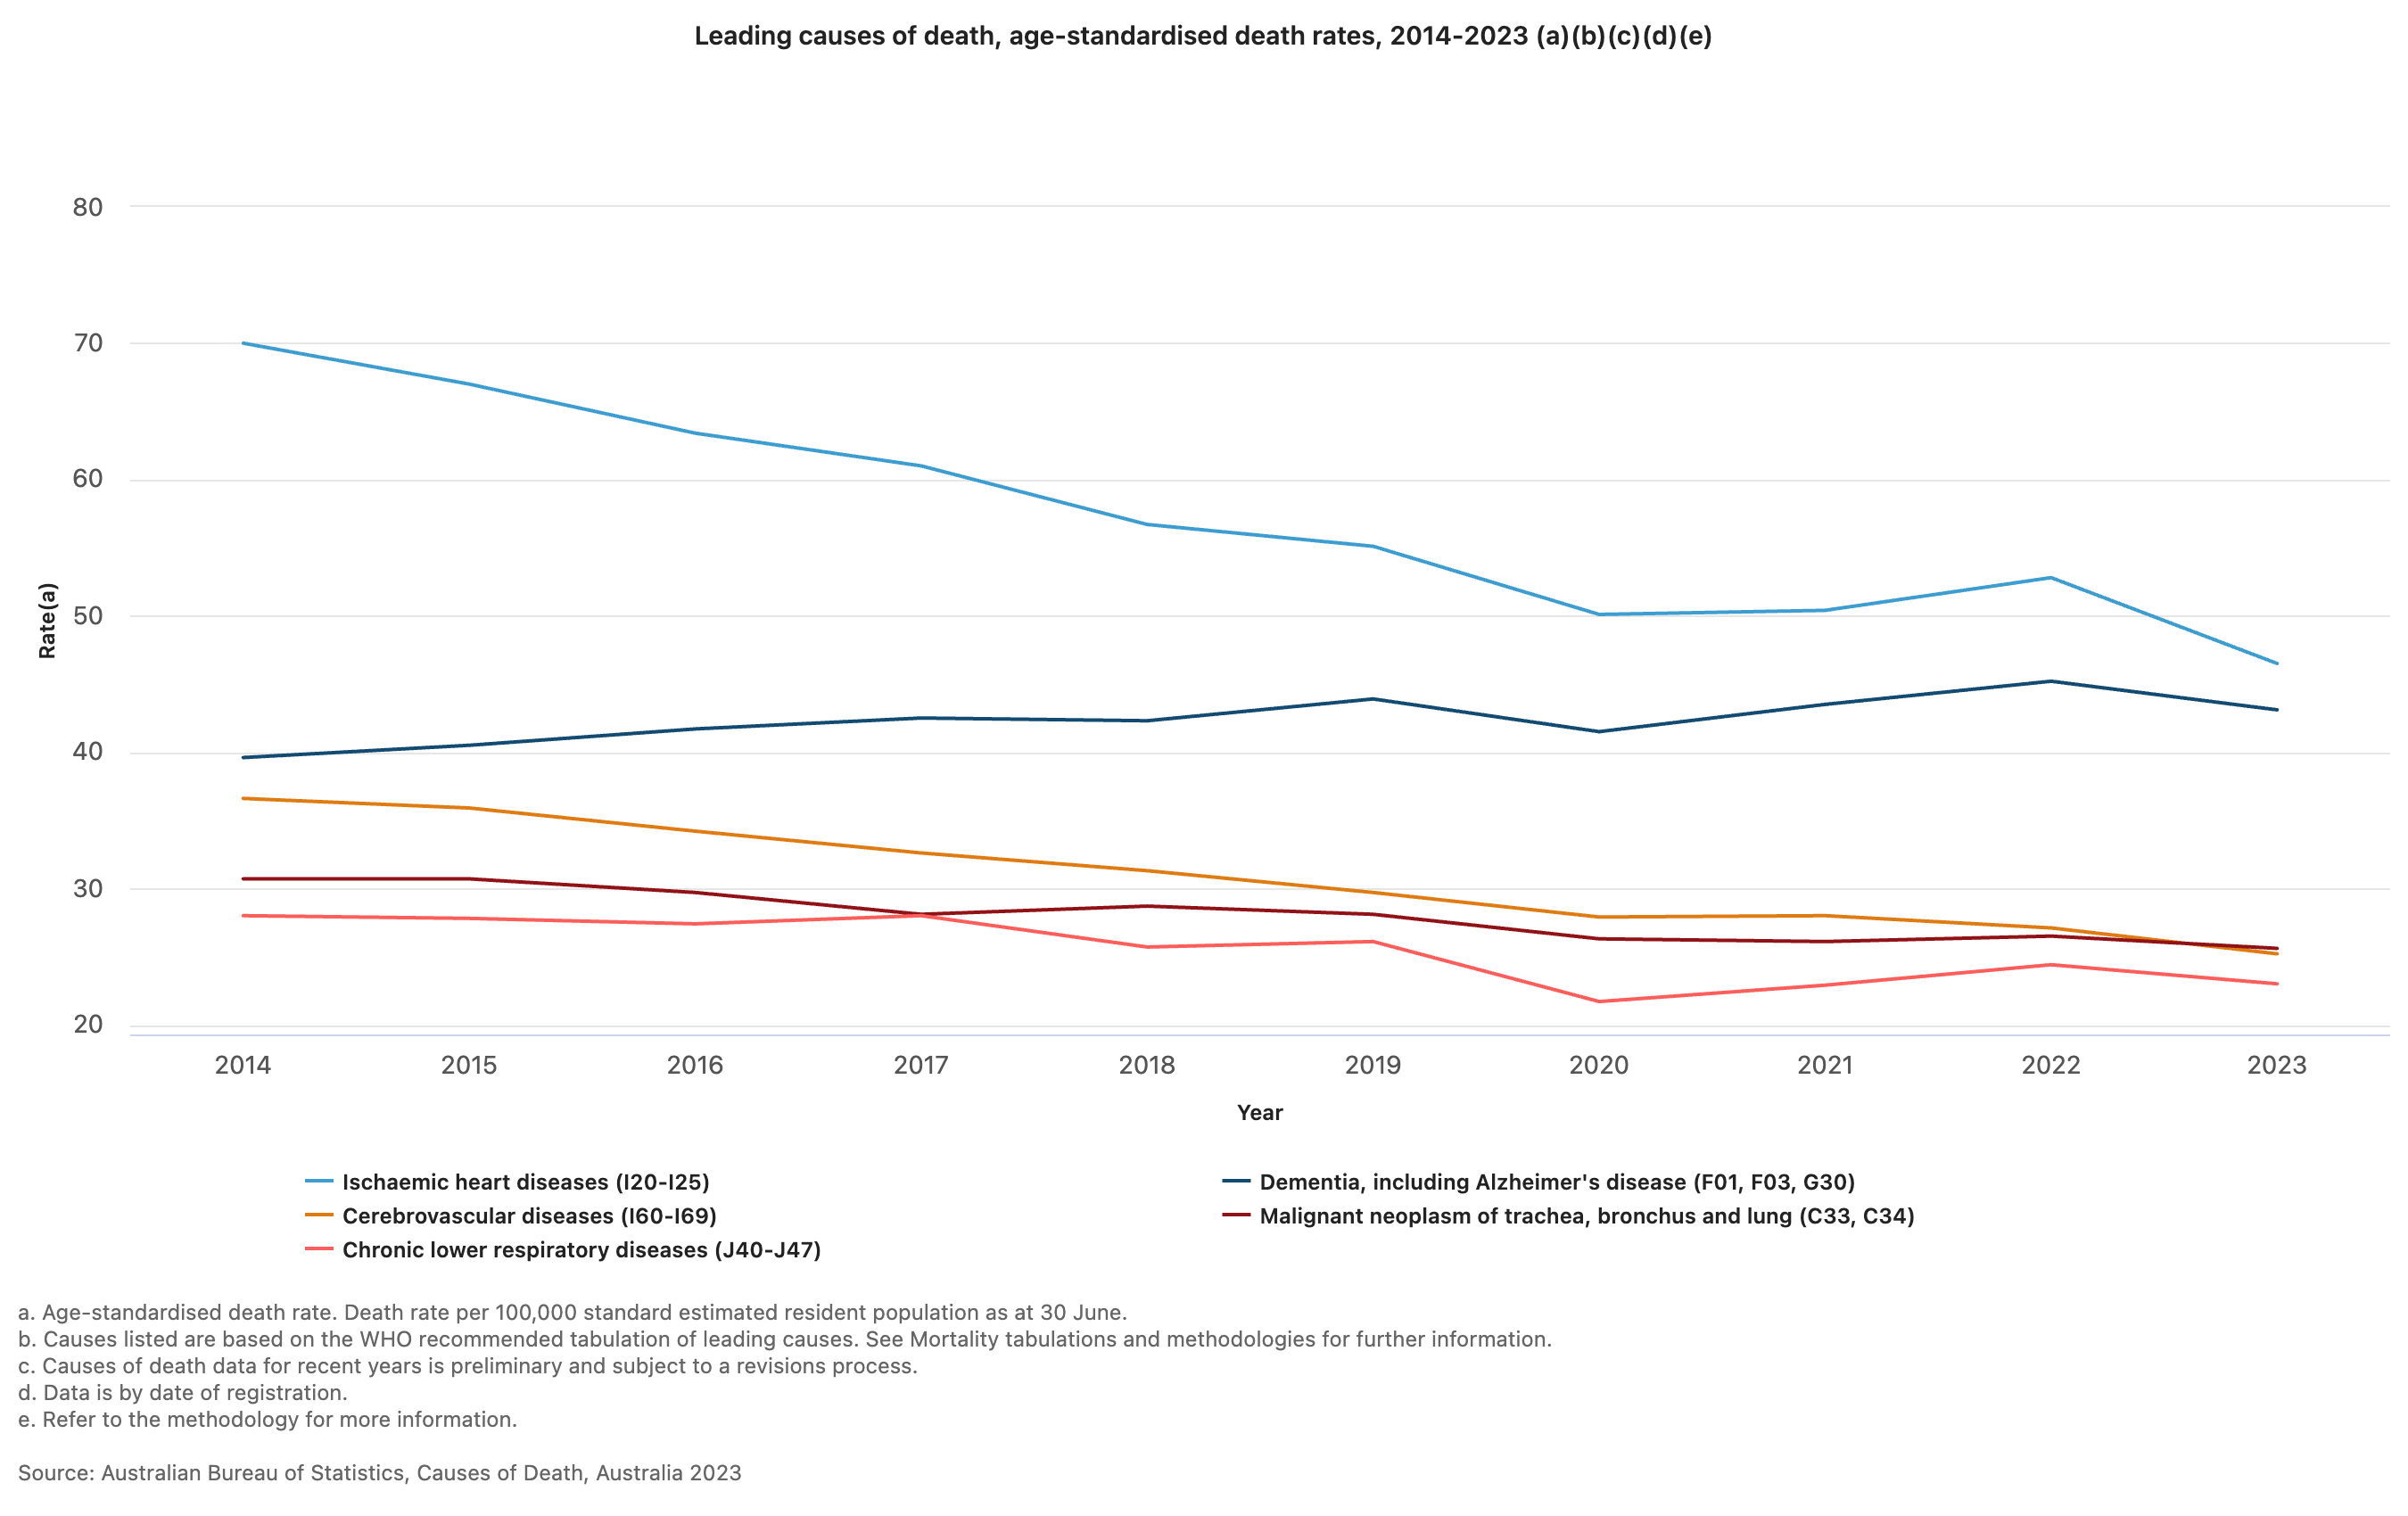
\includegraphics[width=1\textwidth,height=\textheight]{img/mod01/cause-death.png}

}

\caption{\label{fig-1-1}Leading causes of death, age-standardised death
rates, 2014-2023}

\end{figure}

\hypertarget{inferential-statistics}{%
\subsection{Inferential statistics}\label{inferential-statistics}}

Inferential statistics use data collected from a sample to make
conclusions (inferences) about the whole population from which the
sample was drawn. For example, the Australian Institute of Health and
Welfare's \textbf{Australia's health} reports (eg
(\textbf{australianinstituteofhealthandwelfare25?})) use a
representative sample to make estimates of the health of the whole of
Australia. We will revisit \emph{inferential statistics} in later
modules.

\hypertarget{summarising-continuous-data}{%
\section{Summarising continuous
data}\label{summarising-continuous-data}}

In the first two Modules, we will focus on ways to summarise and present
data. We will see that the choice of presentation will depend on the
type of variable being summarised. In this Module, we will focus on
continuous variables, and will focus on categorical data in Module 2.

\hypertarget{summarising-a-single-continuous-variable-numerically}{%
\subsection{Summarising a single continuous variable
numerically}\label{summarising-a-single-continuous-variable-numerically}}

When summarising continuous data numerically, there are two things we
want to know:

\begin{enumerate}
\def\labelenumi{\arabic{enumi}.}
\tightlist
\item
  What is the average value? And,
\item
  How variable (or spread out) are the data?
\end{enumerate}

We will use a sample of 35 ages (in whole years) to illustrate how to
calculate the average value and measures of variability:

59 41 44 43 31 47 53 59 35 60 54 61 67 52 43 46 39 69 50 64 57 39 54 50
51 31 48 49 70 44 60 51 37 53 34

\hypertarget{sec-measures-of-central-tendency}{%
\subsubsection{Measures of central
tendency}\label{sec-measures-of-central-tendency}}

\hypertarget{mean}{%
\subsubsection{Mean}\label{mean}}

The most commonly used measure of the central tendency of the data is
the mean, calculated as:

\[\bar{x} = \frac{\sum x}{n}\]

From the age example: \(\bar{x}\) = 1745/35 = 49.9. Thus, the mean age
of this sample is 49.9 years.

\hypertarget{median}{%
\subsubsection{Median}\label{median}}

Other measures of central tendency include the median and mode. The
median is the middle value of the data, the value at which half of the
measurements lie above it and half of the measurements lie below it.

To estimate the median, the data are ordered from the lowest to highest
values, and the middle value is used. If the middle value is between two
data points (if there are an even number of observations), the median is
an average of the two values.

Using our example, we could rank the ages from smallest to largest, and
locate the middle value (which has been bolded):

31 31 34 35 37 39 39 41 43 43 44 44 46 47 48 49 50 \textbf{50} 51 51 52
53 53 54 54 57 59 59 60 60 61 64 67 69 70

Here, the median age is 50 years.

Note that, in practice, the median is usually calculated by software
automatically, and there is no need to rank our data.

\hypertarget{describing-the-spread-of-the-data}{%
\subsubsection{Describing the spread of the
data}\label{describing-the-spread-of-the-data}}

In addition to measuring the centre of the data, we also need an
estimate of the variability, or spread, of the data points.

\hypertarget{range}{%
\subsubsection{Range}\label{range}}

The absolute measure of the spread of the data is the range, that is the
difference between the highest and lowest values in the dataset.

Range = highest data value -- lowest data value

Using the age example, Range = 70 - 31 = 39 years.

The range is most usefully reported as the actual lowest and highest
values e.g.~Range: 31 to 70 years.

The range is not always ideal as it only describes the extreme values,
without considering how the bulk of the data is distributed between
them.

\hypertarget{variance-and-standard-deviation}{%
\subsubsection{Variance and standard
deviation}\label{variance-and-standard-deviation}}

More useful statistics to describe the spread of the data around a mean
value are the variance and standard deviation. These measures of
variability depend on the difference between individual observations and
the mean value (deviations). If all values are equal to the mean there
would be no variability at all, all deviations would be zero; conversely
large deviations indicate greater variability.

One way of combining deviations in a single measure is to first square
the deviations and then average the squares. Squaring is done because we
are equally interested in negative deviations and positive deviations;
if we averaged without squaring, negative and positive deviations would
`cancel out'. This measure is called the variance of the set of
observations. It is `the average squared deviation from the mean'.
Because the variance is in `square' units and not in the units of the
measurement, a second measure is derived by taking the square root of
the variance. This is the standard deviation (SD), and is the most
commonly used measure of variability in practice, as it is a more
intuitive interpretation since it is in the same units as the units of
measurement.

The formula for the variance of a sample (\(s^2\)) is:

\[ s^2 = \frac{\sum(x - \bar{x})^2}{n-1} \]

Note that the deviations are first squared before they are summed to
remove the negative values; once summed they are divided by the sample
size minus 1.

The sample standard deviation is the square root of the of the sample
variance:

\[s = \sqrt{s^2}\] For the age example, we would calculate the sample
variance using statistical software. The sample standard deviation is
estimated as: \(s = 10.47 \text{ years}\).

Characteristics of the standard deviation:

\begin{itemize}
\tightlist
\item
  It is affected by every measurement
\item
  It is in the same units as the measurements
\item
  It can be converted to measures of precision (standard error and 95\%
  confidence intervals) (Module 3)
\end{itemize}

\hypertarget{interquartile-range}{%
\subsubsection{Interquartile range}\label{interquartile-range}}

The inter-quartile range (IQR) describes the range of measurements in
the central 50\% of values lie. This is estimated by calculating the
values that cut the data at the bottom 25\% and top 25\%. The IQR is the
preferred measure of spread when the median has been used to describe
central tendency.

In the age example, the IQR is estimated as 43 to 59 years. Note that R
and Stata use slightly different methods to calculate the interquartile
range (Stata IQR: 43 to 59 years; R IQR: 43 to 58 years). This
difference is not practically important, and either range would be
considered correct.

\hypertarget{population-values-mean-variance-and-standard-deviation}{%
\subsubsection{Population values: mean, variance and standard
deviation}\label{population-values-mean-variance-and-standard-deviation}}

The examples above show how the sample mean, range, variance and
standard deviation are calculated from the sample of ages from 35
people. If we had information on the age of the \emph{entire} population
that the sample was drawn from, we could calculate all the summary
statistics described above (for the sample) for the population.

The equation for calculating the population mean is the same as that of
sample mean, though now we denote the population mean as \(\mu\):

\[ \mu = \frac{\sum{x}}{N} \]

Where \(\sum{x}\) represents the sum of the values in the population,
and \(N\) represents the total number of measurements in the population.

To calculate the population variance (\(\sigma^2\)) and standard
deviation(\(\sigma\)), we use a slightly modified version of the
equation for \(s^2\):

\[ \sigma^2 = \frac{\sum(x - \mu)^2}{N} \]

with a population standard deviation of: \(\sigma = \sqrt{\sigma^2}\).

In practice, we rarely have the information for the entire population to
be able to calculate the population mean and standard deviation.
Theoretically, however, these statistics are important for two main
purposes:

\begin{enumerate}
\def\labelenumi{\arabic{enumi}.}
\tightlist
\item
  the characteristics of the normal distribution (the most important
  probability distribution discussed in later modules) are defined by
  the population mean and standard deviation;
\item
  while calculating sample sizes (discussed in later modules) we need
  information about the population standard deviation, which is usually
  obtained from the existing literature.
\end{enumerate}

\hypertarget{summarising-a-single-continuous-variable-graphically}{%
\subsection{Summarising a single continuous variable
graphically}\label{summarising-a-single-continuous-variable-graphically}}

As well as calculating measures of central tendency and spread to
describe the characteristics of the data, a graphical plot can be
helpful to better understand the characteristics and distribution of the
measurements obtained. \emph{Histograms, density plots} and \emph{box
plots} are excellent ways to display continuous data graphically.

\hypertarget{frequency-histograms}{%
\subsubsection{Frequency histograms}\label{frequency-histograms}}

A frequency histogram is a plot of the number of observations that fall
within defined ranges of non-overlapping intervals (called bins).
Examples of frequency histograms are given in Figure~\ref{fig-hist-1}.

\begin{figure}

{\centering 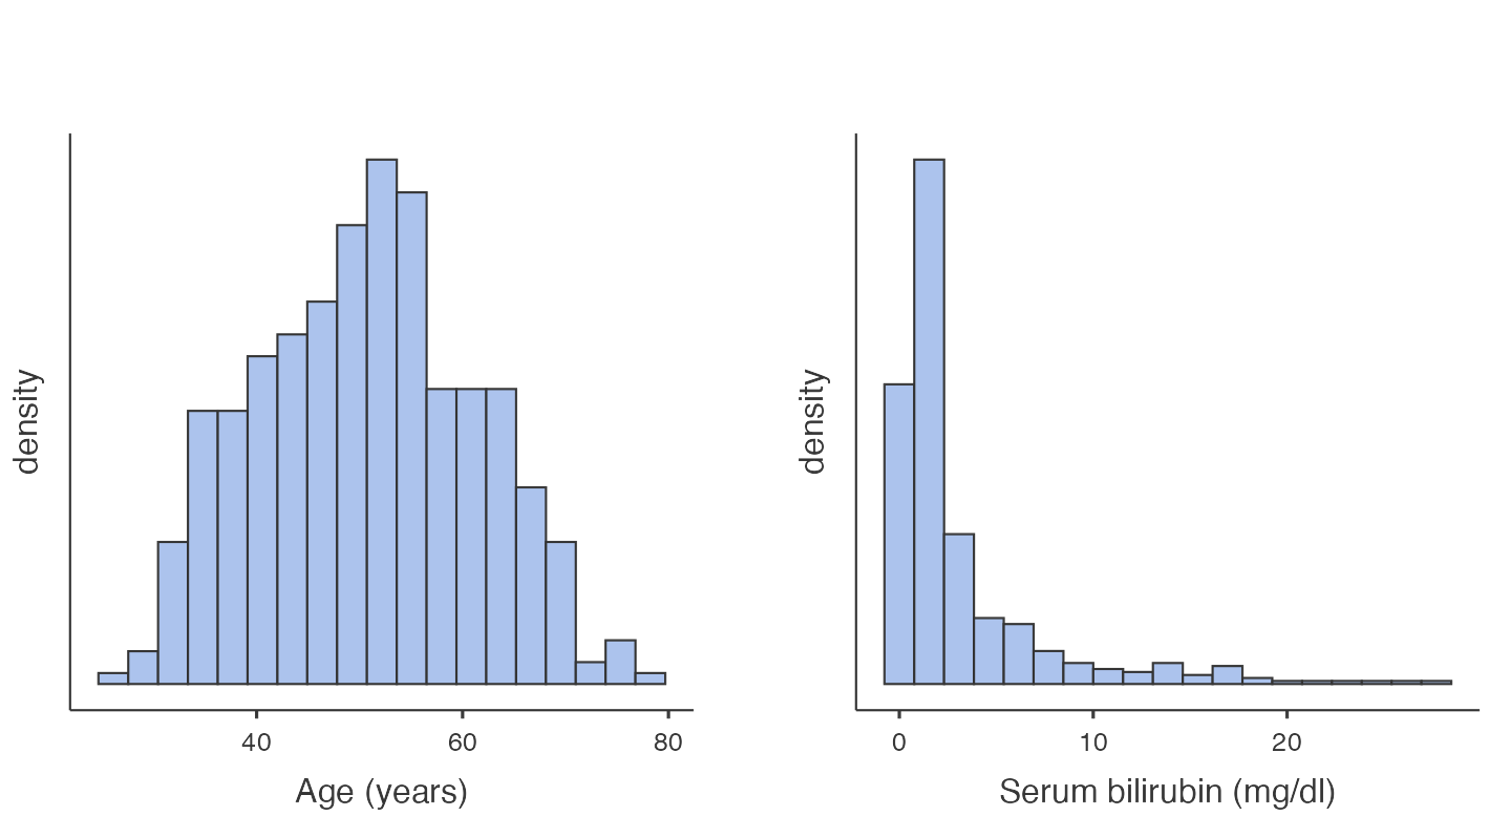
\includegraphics[width=1\textwidth,height=\textheight]{img/mod01/hist-symmetric-skewed.png}

}

\caption{\label{fig-hist-1}Histogram of age (left) and serum bilirubin
(right) from a sample of data}

\end{figure}

Some features of a frequency histogram:

\begin{itemize}
\tightlist
\item
  The area under each rectangle is proportional to the frequency
\item
  The rectangles are drawn without gaps between them (that is, the
  rectangles touch)
\item
  The data are `binned' into discrete intervals (usually of equal width)
\end{itemize}

A slight variation on the frequency histogram is the \textbf{density
histogram}, which plots the density on the y-axis. The density is a
technical term, which is similar to the relative frequency, but is
scaled so that the sum of the area of the bars is equal to 1.

Both the frequency and density histograms are useful for understanding
how the data is distributed across the range of values. Taller bars
indicate regions where the data is more densely concentrated, while
shorter bars represent areas with fewer data points.

\hypertarget{density-plot}{%
\subsubsection{Density plot}\label{density-plot}}

A density plot can be thought of as a smoothed version of a density
histogram. Like histograms, density plots show areas where there are a
lot of observations and areas where there are relatively few
observations. Figure~\ref{fig-dens-1} illustrates example density plots
for the same data as plotted in Figure~\ref{fig-hist-1}.

\begin{figure}

{\centering 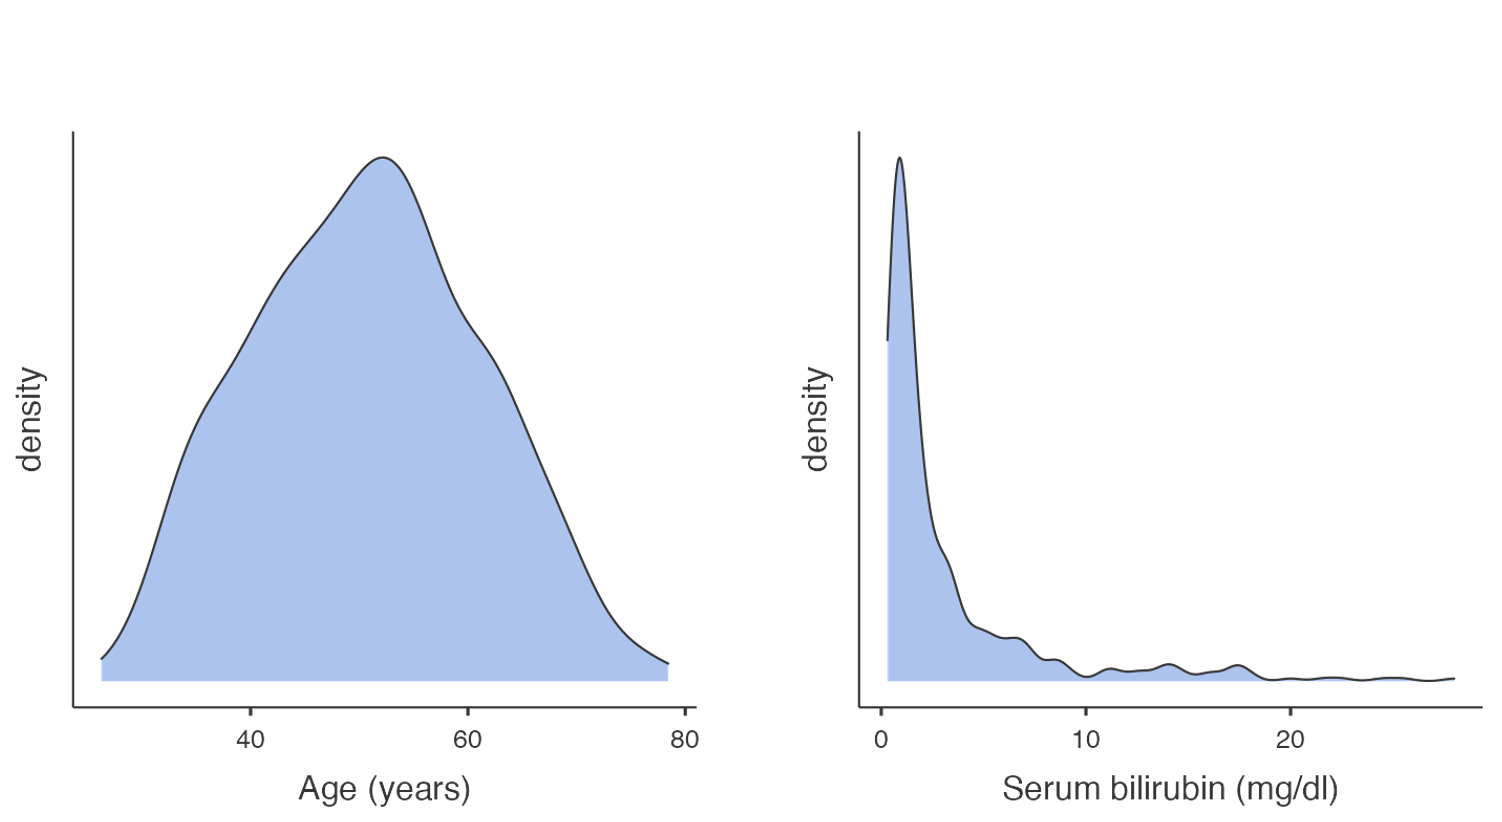
\includegraphics[width=1\textwidth,height=\textheight]{img/mod01/dens-symmetric-skewed.png}

}

\caption{\label{fig-dens-1}Histogram of age (left) and serum bilirubin
(right) from a sample of data}

\end{figure}

Like histograms, density plots allow you to see the overall shape of a
distribution. They are most useful when there are only a small number of
observations being plotted. When plotting small datasets, the shape of a
histogram can depend on how the bins are defined. This is less of an
issue if a density plot is used.

\hypertarget{boxplots}{%
\subsubsection{Boxplots}\label{boxplots}}

Another way to inspect the distribution of data is by using a box plot.
In a box plot:

\begin{itemize}
\tightlist
\item
  the line across the box shows the median value
\item
  the limits of the box show the 25-75\% range (i.e.~the inter-quartile
  range (IQR) where the middle 50\% of the data lie)
\item
  the bars (or whiskers) indicate the most extreme values (highest and
  lowest) that fall within 1.5 times the interquartile range from each
  end of the box

  \begin{itemize}
  \tightlist
  \item
    the upper whisker is the highest value falling within 75th
    percentile plus 1.5 × IQR
  \item
    the lower whisker is the lowest value falling within 25th percentile
    minus 1.5 × IQR
  \end{itemize}
\item
  any values in the dataset lying outside the whiskers are plotted
  individually.
\end{itemize}

Figure~\ref{fig-box-1} presents two example boxplots for age and serum
bilirubin.

\begin{figure}

{\centering 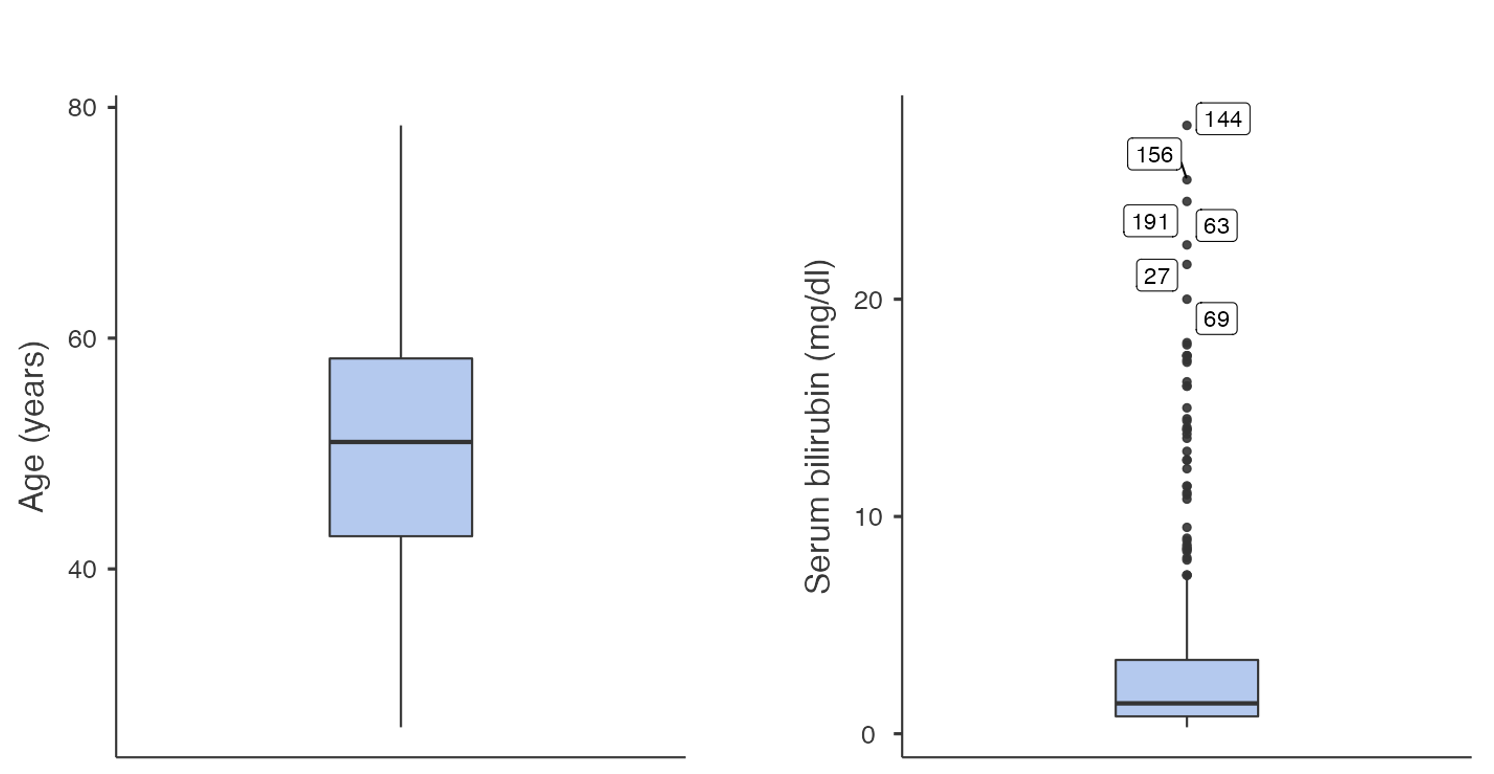
\includegraphics[width=1\textwidth,height=\textheight]{img/mod01/boxp-symmetric-skewed.png}

}

\caption{\label{fig-box-1}Box plot of age (left) and serum bilirubin
(right) from PBC study data}

\end{figure}

\hypertarget{the-shape-of-a-distribution}{%
\subsection{The shape of a
distribution}\label{the-shape-of-a-distribution}}

Histograms and density plots allow us to consider the shape of a
distribution, and in particular, whether a distribution is
\emph{symmetric} or \emph{skewed}.

In a histogram, if the rectangles fall in a roughly symmetric shape
around a single midpoint, we say that the distribution is symmetric.
Similarly, if a density plot looks roughly symmetric around a single
point, the distribution is symmetric.

If the histogram or density plot has a longer tail to the right, then
the data are said to be positively skewed (or skewed to the right); if
the histogram or density plot has an extended tail to the left, then the
data are negatively skewed (or skewed to the left).

\begin{quote}
The skewness of a distribution is defined by the location of the longer
tail in a histogram or density plot, not the location of the peak of the
data.
\end{quote}

From Figure~\ref{fig-hist-1} and Figure~\ref{fig-dens-1}, we can see
that the distribution for age is roughly symmetric, while the
distribution for serum bilirubin is highly positively skewed (or skewed
to the right).

While it is technically possible to determine the shape of a
distribution using a boxplot, a histogram or density plot gives a more
complete illustration of a distribution and would be the preferred
method of assessing shape.

\hypertarget{which-measure-of-central-tendency-to-use}{%
\subsection{Which measure of central tendency to
use}\label{which-measure-of-central-tendency-to-use}}

We introduced the mean and median in
Section~\ref{sec-measures-of-central-tendency} as measures of central
tendency. We need to assess the shape of a distribution to answer which
is the more appropriate measure to use.

If a distribution is symmetric, the mean and median will be
approximately equal. However, the mean is the preferred measure of
central tendency as it makes use of every data point, and has more
useful mathematical properties.

The mean is not a good measure of central tendency for skewed
distributions, as the calculation will be influenced by the observations
in the tail of the distribution. The median is the preferred statistic
for describing central tendency in a skewed distribution.

If the data exhibits a symmetric distribution, we use the standard
deviation as the measure of spread. Otherwise, the interquartile range
is preferred.

\bookmarksetup{startatroot}

\hypertarget{probability-and-probability-distributions}{%
\chapter{Probability and probability
distributions}\label{probability-and-probability-distributions}}

\hypertarget{learning-objectives-1}{%
\section*{Learning objectives}\label{learning-objectives-1}}
\addcontentsline{toc}{section}{Learning objectives}

\markright{Learning objectives}

By the end of this module you will be able to:

\begin{itemize}
\tightlist
\item
  Describe the concept of probability;
\item
  Describe the characteristics of a binomial distribution and a Normal
  distribution;
\item
  Compute probabilities from a binomial distribution using statistical
  software;
\item
  Compute probabilities from a Normal distribution using statistical
  software;
\item
  Decide when to use parametric or non-parametric statistical methods;
\item
  Briefly outline other types of distributions.
\end{itemize}

\hypertarget{optional-readings-1}{%
\section*{Optional readings}\label{optional-readings-1}}
\addcontentsline{toc}{section}{Optional readings}

\markright{Optional readings}

Kirkwood and Sterne (2001); Chapters 5, 14 and 15.
\href{http://er1.library.unsw.edu.au/er/cgi-bin/eraccess.cgi?url=https://ebookcentral.proquest.com/lib/unsw/detail.action?docID=624728}{{[}UNSW
Library Link{]}}

Bland (2015); Chapters 6 and 7.
\href{http://er1.library.unsw.edu.au/er/cgi-bin/eraccess.cgi?url=https://ebookcentral.proquest.com/lib/unsw/detail.action?docID=5891730}{{[}UNSW
Library Link{]}}

\hypertarget{introduction}{%
\section{Introduction}\label{introduction}}

In Module 1, we looked at how to summarise data numerically and
graphically. In this module, we will introduce the concept of
probability which underpins the theoretical basis of statistics, and
then introduce the concept of probability distributions. We will look at
the binomial distribution, and then look at the most important
distribution in statistics: the Normal distribution. Finally, we
introduce some other probability distributions commonly used in
biostatistics.

\hypertarget{summarising-a-single-categorical-variable-numerically}{%
\subsection{Summarising a single categorical variable
numerically}\label{summarising-a-single-categorical-variable-numerically}}

Categorical data are best summarised using a frequency table, where each
category is summarised by its frequency: the count of the number of
individuals in each category. The \textbf{relative frequency} (the
frequency expressed as a proportion or percentage of the total
frequency) is usually included give further insight.

\hypertarget{tbl-1-sex}{}
\global\setlength{\Oldarrayrulewidth}{\arrayrulewidth}

\global\setlength{\Oldtabcolsep}{\tabcolsep}

\setlength{\tabcolsep}{2pt}

\renewcommand*{\arraystretch}{1.5}



\providecommand{\ascline}[3]{\noalign{\global\arrayrulewidth #1}\arrayrulecolor[HTML]{#2}\cline{#3}}

\begin{longtable}[c]{|p{1.00in}|p{1.00in}|p{1.50in}}
\caption{\label{tbl-1-sex}Sex of participants in PBC study }\tabularnewline




\ascline{1.5pt}{666666}{1-3}

\multicolumn{1}{>{\raggedright}m{\dimexpr 1in+0\tabcolsep}}{\textcolor[HTML]{000000}{\fontsize{11}{11}\selectfont{\global\setmainfont{Helvetica}{Sex}}}} & \multicolumn{1}{>{\raggedleft}m{\dimexpr 1in+0\tabcolsep}}{\textcolor[HTML]{000000}{\fontsize{11}{11}\selectfont{\global\setmainfont{Helvetica}{Frequency}}}} & \multicolumn{1}{>{\raggedleft}m{\dimexpr 1.5in+0\tabcolsep}}{\textcolor[HTML]{000000}{\fontsize{11}{11}\selectfont{\global\setmainfont{Helvetica}{Relative\ frequency\ (\%)}}}} \\

\ascline{1.5pt}{666666}{1-3}\endfirsthead 

\ascline{1.5pt}{666666}{1-3}

\multicolumn{1}{>{\raggedright}m{\dimexpr 1in+0\tabcolsep}}{\textcolor[HTML]{000000}{\fontsize{11}{11}\selectfont{\global\setmainfont{Helvetica}{Sex}}}} & \multicolumn{1}{>{\raggedleft}m{\dimexpr 1in+0\tabcolsep}}{\textcolor[HTML]{000000}{\fontsize{11}{11}\selectfont{\global\setmainfont{Helvetica}{Frequency}}}} & \multicolumn{1}{>{\raggedleft}m{\dimexpr 1.5in+0\tabcolsep}}{\textcolor[HTML]{000000}{\fontsize{11}{11}\selectfont{\global\setmainfont{Helvetica}{Relative\ frequency\ (\%)}}}} \\

\ascline{1.5pt}{666666}{1-3}\endhead



\multicolumn{1}{>{\raggedright}m{\dimexpr 1in+0\tabcolsep}}{\textcolor[HTML]{000000}{\fontsize{11}{11}\selectfont{\global\setmainfont{Helvetica}{Male}}}} & \multicolumn{1}{>{\raggedleft}m{\dimexpr 1in+0\tabcolsep}}{\textcolor[HTML]{000000}{\fontsize{11}{11}\selectfont{\global\setmainfont{Helvetica}{44}}}} & \multicolumn{1}{>{\raggedleft}m{\dimexpr 1.5in+0\tabcolsep}}{\textcolor[HTML]{000000}{\fontsize{11}{11}\selectfont{\global\setmainfont{Helvetica}{10.5}}}} \\





\multicolumn{1}{>{\raggedright}m{\dimexpr 1in+0\tabcolsep}}{\textcolor[HTML]{000000}{\fontsize{11}{11}\selectfont{\global\setmainfont{Helvetica}{Female}}}} & \multicolumn{1}{>{\raggedleft}m{\dimexpr 1in+0\tabcolsep}}{\textcolor[HTML]{000000}{\fontsize{11}{11}\selectfont{\global\setmainfont{Helvetica}{374}}}} & \multicolumn{1}{>{\raggedleft}m{\dimexpr 1.5in+0\tabcolsep}}{\textcolor[HTML]{000000}{\fontsize{11}{11}\selectfont{\global\setmainfont{Helvetica}{89.5}}}} \\

\ascline{1.5pt}{666666}{1-3}



\end{longtable}



\arrayrulecolor[HTML]{000000}

\global\setlength{\arrayrulewidth}{\Oldarrayrulewidth}

\global\setlength{\tabcolsep}{\Oldtabcolsep}

\renewcommand*{\arraystretch}{1}

It is sometimes useful to present the cumulative relative frequency,
which shows the relative frequency of individuals in a certain category
or below (for example, Table~\ref{tbl-1-stage}).

\hypertarget{tbl-1-stage}{}
 
  \providecommand{\huxb}[2]{\arrayrulecolor[RGB]{#1}\global\arrayrulewidth=#2pt}
  \providecommand{\huxvb}[2]{\color[RGB]{#1}\vrule width #2pt}
  \providecommand{\huxtpad}[1]{\rule{0pt}{#1}}
  \providecommand{\huxbpad}[1]{\rule[-#1]{0pt}{#1}}

\begin{table}[ht]
\caption{\label{tbl-1-stage}Stage of disease for participants in PBC study }\tabularnewline

\begin{centerbox}
\begin{threeparttable}
 
\setlength{\tabcolsep}{0pt}
\begin{tabularx}{0.8\textwidth}{p{0.2\textwidth} p{0.2\textwidth} p{0.2\textwidth} p{0.2\textwidth}}


\hhline{>{\huxb{0, 0, 0}{0.4}}->{\huxb{0, 0, 0}{0.4}}->{\huxb{0, 0, 0}{0.4}}->{\huxb{0, 0, 0}{0.4}}-}
\arrayrulecolor{black}

\multicolumn{1}{!{\huxvb{0, 0, 0}{0}}p{0.2\textwidth}!{\huxvb{0, 0, 0}{0}}}{\hspace{0pt}\parbox[b]{0.2\textwidth-0pt-6pt}{\huxtpad{6pt + 1em}\raggedright \textbf{Stage *}\huxbpad{6pt}}} &
\multicolumn{1}{p{0.2\textwidth}!{\huxvb{0, 0, 0}{0}}}{\hspace{6pt}\parbox[b]{0.2\textwidth-6pt-6pt}{\huxtpad{6pt + 1em}\raggedleft \textbf{Frequency}\huxbpad{6pt}}} &
\multicolumn{1}{p{0.2\textwidth}!{\huxvb{0, 0, 0}{0}}}{\hspace{6pt}\parbox[b]{0.2\textwidth-6pt-6pt}{\huxtpad{6pt + 1em}\raggedleft \textbf{Relative frequency (\%)}\huxbpad{6pt}}} &
\multicolumn{1}{p{0.2\textwidth}!{\huxvb{0, 0, 0}{0}}}{\hspace{6pt}\parbox[b]{0.2\textwidth-6pt-0pt}{\huxtpad{6pt + 1em}\raggedleft \textbf{Cumulative relative frequency (\%)}\huxbpad{6pt}}} \tabularnewline[-0.5pt]


\hhline{>{\huxb{0, 0, 0}{0.4}}->{\huxb{0, 0, 0}{0.4}}->{\huxb{0, 0, 0}{0.4}}->{\huxb{0, 0, 0}{0.4}}-}
\arrayrulecolor{black}

\multicolumn{1}{!{\huxvb{0, 0, 0}{0}}p{0.2\textwidth}!{\huxvb{0, 0, 0}{0}}}{\hspace{0pt}\parbox[b]{0.2\textwidth-0pt-6pt}{\huxtpad{6pt + 1em}\raggedright 1\huxbpad{6pt}}} &
\multicolumn{1}{p{0.2\textwidth}!{\huxvb{0, 0, 0}{0}}}{\hspace{6pt}\parbox[b]{0.2\textwidth-6pt-6pt}{\huxtpad{6pt + 1em}\raggedleft 21\huxbpad{6pt}}} &
\multicolumn{1}{p{0.2\textwidth}!{\huxvb{0, 0, 0}{0}}}{\hspace{6pt}\parbox[b]{0.2\textwidth-6pt-6pt}{\huxtpad{6pt + 1em}\raggedleft 5.1\huxbpad{6pt}}} &
\multicolumn{1}{p{0.2\textwidth}!{\huxvb{0, 0, 0}{0}}}{\hspace{6pt}\parbox[b]{0.2\textwidth-6pt-0pt}{\huxtpad{6pt + 1em}\raggedleft 5.1\huxbpad{6pt}}} \tabularnewline[-0.5pt]


\hhline{}
\arrayrulecolor{black}

\multicolumn{1}{!{\huxvb{0, 0, 0}{0}}p{0.2\textwidth}!{\huxvb{0, 0, 0}{0}}}{\hspace{0pt}\parbox[b]{0.2\textwidth-0pt-6pt}{\huxtpad{6pt + 1em}\raggedright 2\huxbpad{6pt}}} &
\multicolumn{1}{p{0.2\textwidth}!{\huxvb{0, 0, 0}{0}}}{\hspace{6pt}\parbox[b]{0.2\textwidth-6pt-6pt}{\huxtpad{6pt + 1em}\raggedleft 92\huxbpad{6pt}}} &
\multicolumn{1}{p{0.2\textwidth}!{\huxvb{0, 0, 0}{0}}}{\hspace{6pt}\parbox[b]{0.2\textwidth-6pt-6pt}{\huxtpad{6pt + 1em}\raggedleft 22.3\huxbpad{6pt}}} &
\multicolumn{1}{p{0.2\textwidth}!{\huxvb{0, 0, 0}{0}}}{\hspace{6pt}\parbox[b]{0.2\textwidth-6pt-0pt}{\huxtpad{6pt + 1em}\raggedleft 27.4\huxbpad{6pt}}} \tabularnewline[-0.5pt]


\hhline{}
\arrayrulecolor{black}

\multicolumn{1}{!{\huxvb{0, 0, 0}{0}}p{0.2\textwidth}!{\huxvb{0, 0, 0}{0}}}{\hspace{0pt}\parbox[b]{0.2\textwidth-0pt-6pt}{\huxtpad{6pt + 1em}\raggedright 3\huxbpad{6pt}}} &
\multicolumn{1}{p{0.2\textwidth}!{\huxvb{0, 0, 0}{0}}}{\hspace{6pt}\parbox[b]{0.2\textwidth-6pt-6pt}{\huxtpad{6pt + 1em}\raggedleft 155\huxbpad{6pt}}} &
\multicolumn{1}{p{0.2\textwidth}!{\huxvb{0, 0, 0}{0}}}{\hspace{6pt}\parbox[b]{0.2\textwidth-6pt-6pt}{\huxtpad{6pt + 1em}\raggedleft 37.6\huxbpad{6pt}}} &
\multicolumn{1}{p{0.2\textwidth}!{\huxvb{0, 0, 0}{0}}}{\hspace{6pt}\parbox[b]{0.2\textwidth-6pt-0pt}{\huxtpad{6pt + 1em}\raggedleft 65.0\huxbpad{6pt}}} \tabularnewline[-0.5pt]


\hhline{}
\arrayrulecolor{black}

\multicolumn{1}{!{\huxvb{0, 0, 0}{0}}p{0.2\textwidth}!{\huxvb{0, 0, 0}{0}}}{\hspace{0pt}\parbox[b]{0.2\textwidth-0pt-6pt}{\huxtpad{6pt + 1em}\raggedright 4\huxbpad{6pt}}} &
\multicolumn{1}{p{0.2\textwidth}!{\huxvb{0, 0, 0}{0}}}{\hspace{6pt}\parbox[b]{0.2\textwidth-6pt-6pt}{\huxtpad{6pt + 1em}\raggedleft 144\huxbpad{6pt}}} &
\multicolumn{1}{p{0.2\textwidth}!{\huxvb{0, 0, 0}{0}}}{\hspace{6pt}\parbox[b]{0.2\textwidth-6pt-6pt}{\huxtpad{6pt + 1em}\raggedleft 35.0\huxbpad{6pt}}} &
\multicolumn{1}{p{0.2\textwidth}!{\huxvb{0, 0, 0}{0}}}{\hspace{6pt}\parbox[b]{0.2\textwidth-6pt-0pt}{\huxtpad{6pt + 1em}\raggedleft 100.0\huxbpad{6pt}}} \tabularnewline[-0.5pt]


\hhline{>{\huxb{0, 0, 0}{0.8}}->{\huxb{0, 0, 0}{0.8}}->{\huxb{0, 0, 0}{0.8}}->{\huxb{0, 0, 0}{0.8}}-}
\arrayrulecolor{black}

\multicolumn{4}{!{\huxvb{0, 0, 0}{0}}p{0.8\textwidth+6\tabcolsep}!{\huxvb{0, 0, 0}{0}}}{\hspace{6pt}\parbox[b]{0.8\textwidth+6\tabcolsep-6pt-6pt}{\huxtpad{6pt + 1em}\raggedright * Disease stage was missing for 6 participants\huxbpad{6pt}}} \tabularnewline[-0.5pt]


\hhline{}
\arrayrulecolor{black}
\end{tabularx}
\end{threeparttable}\par\end{centerbox}

\end{table}
 

From Table~\ref{tbl-1-stage}, we can see that 65.0\% of participants had
Stage 3 disease or lower.

\hypertarget{summarising-a-single-categorical-variable-graphically}{%
\subsection{Summarising a single categorical variable
graphically}\label{summarising-a-single-categorical-variable-graphically}}

A categorical variable is best summarised graphically using a
\textbf{bar chart}. For example, we can present the distribution of
Stage of Disease graphically using a bar graph (Figure~\ref{fig-bar-1}).
Bar graphs, which are suitable for plotting discrete or categorical
variables, are defined by the fact that the bars do not touch.

\begin{figure}[H]

{\centering 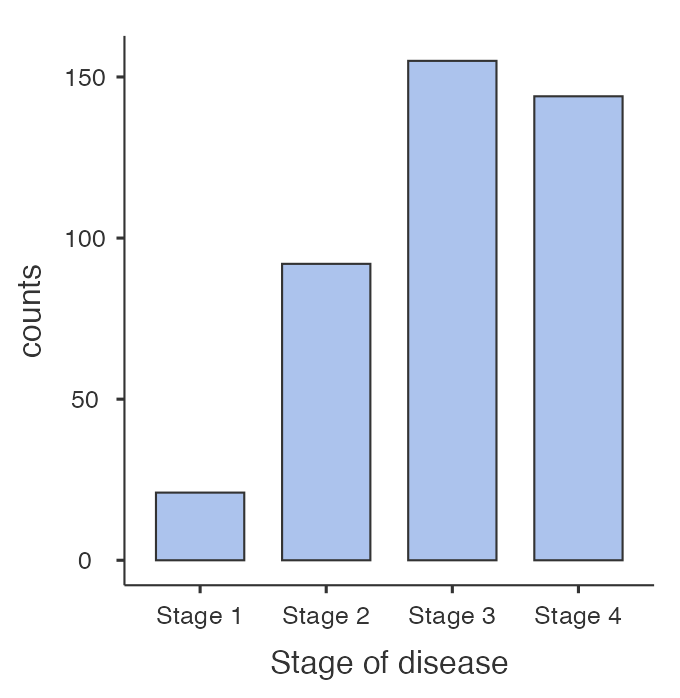
\includegraphics[width=0.75\textwidth,height=\textheight]{img/mod01/pbc-bar.png}

}

\caption{\label{fig-bar-1}Bar graph of stage of disease from PBC study}

\end{figure}

Pie charts can be an alternative way to summarise a categorical variable
graphically, however their use is not recommended for the following
reasons:

\begin{itemize}
\tightlist
\item
  Not ideal when there are many categories to compare
\item
  The use of percentages is not appropriate when the sample size is
  small
\item
  Can be misleading by using different size pies, different rotations
  and different colours to draw attention to specific groups
\item
  3D and exploding bar charts further distort the effect of perspective
  and may confuse the reader
\end{itemize}

Pie charts will not be discussed further in this course.

\hypertarget{summarising-two-categorical-variables-numerically}{%
\subsection{Summarising two categorical variables
numerically}\label{summarising-two-categorical-variables-numerically}}

So far, we have discussed one-way frequency tables, that is, tables that
summarise one variable. We can summarise more than two categorical
variables in a table -- called a cross tabulation, or a two-way
(summarising two variables) table.

Using our PBC data, we can summarise the two categorical variables: sex
and stage of disease. The two-way table of frequencies is shown in
Table~\ref{tbl-1-sex-stage-freq}.

\hypertarget{tbl-1-sex-stage-freq}{}
\global\setlength{\Oldarrayrulewidth}{\arrayrulewidth}

\global\setlength{\Oldtabcolsep}{\tabcolsep}

\setlength{\tabcolsep}{2pt}

\renewcommand*{\arraystretch}{1.5}



\providecommand{\ascline}[3]{\noalign{\global\arrayrulewidth #1}\arrayrulecolor[HTML]{#2}\cline{#3}}

\begin{longtable}[c]{|p{0.79in}|p{0.46in}|p{0.46in}|p{0.54in}|p{0.54in}|p{0.62in}}
\caption{\label{tbl-1-sex-stage-freq}Frequency of participants by sex and stage of disease* }\tabularnewline




\ascline{1.5pt}{666666}{1-6}

\multicolumn{1}{>{\raggedright}b{\dimexpr 0.79in+0\tabcolsep}}{} & \multicolumn{5}{!{\color[HTML]{666666}\vrule width 1pt}>{\centering}m{\dimexpr 2.62in+8\tabcolsep+1pt}}{\textcolor[HTML]{000000}{\fontsize{11}{11}\selectfont{\global\setmainfont{Helvetica}{Stage\ of\ disease\ *}}}} \\

\ascline{0.75pt}{666666}{2-6}



\multicolumn{1}{>{\raggedright}b{\dimexpr 0.79in+0\tabcolsep}}{\multirow[b]{-2}{*}{\parbox{0.79in}{\raggedright \textcolor[HTML]{000000}{\fontsize{11}{11}\selectfont{\global\setmainfont{Helvetica}{Sex}}}}}} & \multicolumn{1}{!{\color[HTML]{666666}\vrule width 1pt}>{\centering}m{\dimexpr 0.46in+0\tabcolsep}}{\textcolor[HTML]{000000}{\fontsize{11}{11}\selectfont{\global\setmainfont{Helvetica}{1}}}} & \multicolumn{1}{>{\centering}m{\dimexpr 0.46in+0\tabcolsep}}{\textcolor[HTML]{000000}{\fontsize{11}{11}\selectfont{\global\setmainfont{Helvetica}{2}}}} & \multicolumn{1}{>{\centering}m{\dimexpr 0.54in+0\tabcolsep}}{\textcolor[HTML]{000000}{\fontsize{11}{11}\selectfont{\global\setmainfont{Helvetica}{3}}}} & \multicolumn{1}{>{\centering}m{\dimexpr 0.54in+0\tabcolsep}}{\textcolor[HTML]{000000}{\fontsize{11}{11}\selectfont{\global\setmainfont{Helvetica}{4}}}} & \multicolumn{1}{!{\color[HTML]{666666}\vrule width 1pt}>{\centering}m{\dimexpr 0.62in+0\tabcolsep}}{\textcolor[HTML]{000000}{\fontsize{11}{11}\selectfont{\global\setmainfont{Helvetica}{Total}}}} \\

\ascline{1.5pt}{666666}{1-6}\endfirsthead 

\ascline{1.5pt}{666666}{1-6}

\multicolumn{1}{>{\raggedright}b{\dimexpr 0.79in+0\tabcolsep}}{} & \multicolumn{5}{!{\color[HTML]{666666}\vrule width 1pt}>{\centering}m{\dimexpr 2.62in+8\tabcolsep+1pt}}{\textcolor[HTML]{000000}{\fontsize{11}{11}\selectfont{\global\setmainfont{Helvetica}{Stage\ of\ disease\ *}}}} \\

\ascline{0.75pt}{666666}{2-6}



\multicolumn{1}{>{\raggedright}b{\dimexpr 0.79in+0\tabcolsep}}{\multirow[b]{-2}{*}{\parbox{0.79in}{\raggedright \textcolor[HTML]{000000}{\fontsize{11}{11}\selectfont{\global\setmainfont{Helvetica}{Sex}}}}}} & \multicolumn{1}{!{\color[HTML]{666666}\vrule width 1pt}>{\centering}m{\dimexpr 0.46in+0\tabcolsep}}{\textcolor[HTML]{000000}{\fontsize{11}{11}\selectfont{\global\setmainfont{Helvetica}{1}}}} & \multicolumn{1}{>{\centering}m{\dimexpr 0.46in+0\tabcolsep}}{\textcolor[HTML]{000000}{\fontsize{11}{11}\selectfont{\global\setmainfont{Helvetica}{2}}}} & \multicolumn{1}{>{\centering}m{\dimexpr 0.54in+0\tabcolsep}}{\textcolor[HTML]{000000}{\fontsize{11}{11}\selectfont{\global\setmainfont{Helvetica}{3}}}} & \multicolumn{1}{>{\centering}m{\dimexpr 0.54in+0\tabcolsep}}{\textcolor[HTML]{000000}{\fontsize{11}{11}\selectfont{\global\setmainfont{Helvetica}{4}}}} & \multicolumn{1}{!{\color[HTML]{666666}\vrule width 1pt}>{\centering}m{\dimexpr 0.62in+0\tabcolsep}}{\textcolor[HTML]{000000}{\fontsize{11}{11}\selectfont{\global\setmainfont{Helvetica}{Total}}}} \\

\ascline{1.5pt}{666666}{1-6}\endhead



\multicolumn{1}{>{\raggedright}p{\dimexpr 0.79in+0\tabcolsep}}{\textcolor[HTML]{000000}{\fontsize{11}{11}\selectfont{\global\setmainfont{Helvetica}{Male}}}} & \multicolumn{1}{!{\color[HTML]{666666}\vrule width 1pt}>{\centering}p{\dimexpr 0.46in+0\tabcolsep}}{\textcolor[HTML]{000000}{\fontsize{11}{11}\selectfont{\global\setmainfont{Helvetica}{3}}}\textcolor[HTML]{000000}{\fontsize{11}{11}\selectfont{\global\setmainfont{Helvetica}{}}}} & \multicolumn{1}{>{\centering}p{\dimexpr 0.46in+0\tabcolsep}}{\textcolor[HTML]{000000}{\fontsize{11}{11}\selectfont{\global\setmainfont{Helvetica}{8}}}\textcolor[HTML]{000000}{\fontsize{11}{11}\selectfont{\global\setmainfont{Helvetica}{}}}} & \multicolumn{1}{>{\centering}p{\dimexpr 0.54in+0\tabcolsep}}{\textcolor[HTML]{000000}{\fontsize{11}{11}\selectfont{\global\setmainfont{Helvetica}{16}}}\textcolor[HTML]{000000}{\fontsize{11}{11}\selectfont{\global\setmainfont{Helvetica}{}}}} & \multicolumn{1}{>{\centering}p{\dimexpr 0.54in+0\tabcolsep}}{\textcolor[HTML]{000000}{\fontsize{11}{11}\selectfont{\global\setmainfont{Helvetica}{17}}}\textcolor[HTML]{000000}{\fontsize{11}{11}\selectfont{\global\setmainfont{Helvetica}{}}}} & \multicolumn{1}{!{\color[HTML]{666666}\vrule width 1pt}>{\centering}p{\dimexpr 0.62in+0\tabcolsep}}{\textcolor[HTML]{000000}{\fontsize{11}{11}\selectfont{\global\setmainfont{Helvetica}{44}}}\textcolor[HTML]{000000}{\fontsize{11}{11}\selectfont{\global\setmainfont{Helvetica}{}}}} \\





\multicolumn{1}{>{\raggedright}p{\dimexpr 0.79in+0\tabcolsep}}{\textcolor[HTML]{000000}{\fontsize{11}{11}\selectfont{\global\setmainfont{Helvetica}{Female}}}} & \multicolumn{1}{!{\color[HTML]{666666}\vrule width 1pt}>{\centering}p{\dimexpr 0.46in+0\tabcolsep}}{\textcolor[HTML]{000000}{\fontsize{11}{11}\selectfont{\global\setmainfont{Helvetica}{18}}}\textcolor[HTML]{000000}{\fontsize{11}{11}\selectfont{\global\setmainfont{Helvetica}{}}}} & \multicolumn{1}{>{\centering}p{\dimexpr 0.46in+0\tabcolsep}}{\textcolor[HTML]{000000}{\fontsize{11}{11}\selectfont{\global\setmainfont{Helvetica}{84}}}\textcolor[HTML]{000000}{\fontsize{11}{11}\selectfont{\global\setmainfont{Helvetica}{}}}} & \multicolumn{1}{>{\centering}p{\dimexpr 0.54in+0\tabcolsep}}{\textcolor[HTML]{000000}{\fontsize{11}{11}\selectfont{\global\setmainfont{Helvetica}{139}}}\textcolor[HTML]{000000}{\fontsize{11}{11}\selectfont{\global\setmainfont{Helvetica}{}}}} & \multicolumn{1}{>{\centering}p{\dimexpr 0.54in+0\tabcolsep}}{\textcolor[HTML]{000000}{\fontsize{11}{11}\selectfont{\global\setmainfont{Helvetica}{127}}}\textcolor[HTML]{000000}{\fontsize{11}{11}\selectfont{\global\setmainfont{Helvetica}{}}}} & \multicolumn{1}{!{\color[HTML]{666666}\vrule width 1pt}>{\centering}p{\dimexpr 0.62in+0\tabcolsep}}{\textcolor[HTML]{000000}{\fontsize{11}{11}\selectfont{\global\setmainfont{Helvetica}{368}}}\textcolor[HTML]{000000}{\fontsize{11}{11}\selectfont{\global\setmainfont{Helvetica}{}}}} \\

\ascline{1pt}{666666}{1-6}



\multicolumn{1}{>{\raggedright}p{\dimexpr 0.79in+0\tabcolsep}}{\textcolor[HTML]{000000}{\fontsize{11}{11}\selectfont{\global\setmainfont{Helvetica}{Total}}}} & \multicolumn{1}{!{\color[HTML]{666666}\vrule width 1pt}>{\centering}p{\dimexpr 0.46in+0\tabcolsep}}{\textcolor[HTML]{000000}{\fontsize{11}{11}\selectfont{\global\setmainfont{Helvetica}{21}}}\textcolor[HTML]{000000}{\fontsize{11}{11}\selectfont{\global\setmainfont{Helvetica}{}}}} & \multicolumn{1}{>{\centering}p{\dimexpr 0.46in+0\tabcolsep}}{\textcolor[HTML]{000000}{\fontsize{11}{11}\selectfont{\global\setmainfont{Helvetica}{92}}}\textcolor[HTML]{000000}{\fontsize{11}{11}\selectfont{\global\setmainfont{Helvetica}{}}}} & \multicolumn{1}{>{\centering}p{\dimexpr 0.54in+0\tabcolsep}}{\textcolor[HTML]{000000}{\fontsize{11}{11}\selectfont{\global\setmainfont{Helvetica}{155}}}\textcolor[HTML]{000000}{\fontsize{11}{11}\selectfont{\global\setmainfont{Helvetica}{}}}} & \multicolumn{1}{>{\centering}p{\dimexpr 0.54in+0\tabcolsep}}{\textcolor[HTML]{000000}{\fontsize{11}{11}\selectfont{\global\setmainfont{Helvetica}{144}}}\textcolor[HTML]{000000}{\fontsize{11}{11}\selectfont{\global\setmainfont{Helvetica}{}}}} & \multicolumn{1}{!{\color[HTML]{666666}\vrule width 1pt}>{\centering}p{\dimexpr 0.62in+0\tabcolsep}}{\textcolor[HTML]{000000}{\fontsize{11}{11}\selectfont{\global\setmainfont{Helvetica}{412}}}\textcolor[HTML]{000000}{\fontsize{11}{11}\selectfont{\global\setmainfont{Helvetica}{}}}} \\

\ascline{1.5pt}{666666}{1-6}



\multicolumn{6}{>{\raggedright}m{\dimexpr 3.41in+10\tabcolsep}}{\textcolor[HTML]{000000}{\fontsize{11}{11}\selectfont{\global\setmainfont{Helvetica}{*\ Disease\ stage\ was\ missing\ for\ 6\ participants}}}} \\





\end{longtable}



\arrayrulecolor[HTML]{000000}

\global\setlength{\arrayrulewidth}{\Oldarrayrulewidth}

\global\setlength{\tabcolsep}{\Oldtabcolsep}

\renewcommand*{\arraystretch}{1}

We can add percentages to two-way tables as either \emph{column} or
\emph{row} percents. Using Table~\ref{tbl-1-sex-stage-freq} as an
example, column percents represent the relative frequencies of sex
within each stage (Table~\ref{tbl-1-sex-stage-col}).

\hypertarget{tktk---fix-missing-100-cells}{%
\subsubsection{TKTK - fix missing ``100\%''
cells}\label{tktk---fix-missing-100-cells}}

\hypertarget{tbl-1-sex-stage-col}{}
\global\setlength{\Oldarrayrulewidth}{\arrayrulewidth}

\global\setlength{\Oldtabcolsep}{\tabcolsep}

\setlength{\tabcolsep}{2pt}

\renewcommand*{\arraystretch}{1.5}



\providecommand{\ascline}[3]{\noalign{\global\arrayrulewidth #1}\arrayrulecolor[HTML]{#2}\cline{#3}}

\begin{longtable}[c]{|p{0.79in}|p{0.80in}|p{0.72in}|p{0.72in}|p{0.72in}|p{0.72in}|p{0.62in}}
\caption{\label{tbl-1-sex-stage-col}Frequency of participants by sex and stage of disease*, including column
percents }\tabularnewline




\ascline{1.5pt}{666666}{1-7}

\multicolumn{1}{>{\raggedright}b{\dimexpr 0.79in+0\tabcolsep}}{} & \multicolumn{1}{>{\raggedright}b{\dimexpr 0.8in+0\tabcolsep}}{} & \multicolumn{5}{!{\color[HTML]{666666}\vrule width 1pt}>{\centering}m{\dimexpr 3.5in+8\tabcolsep+1pt}}{\textcolor[HTML]{000000}{\fontsize{11}{11}\selectfont{\global\setmainfont{Helvetica}{Stage\ of\ disease\ *}}}} \\

\ascline{0.75pt}{666666}{3-7}



\multicolumn{1}{>{\raggedright}b{\dimexpr 0.79in+0\tabcolsep}}{\multirow[b]{-2}{*}{\parbox{0.79in}{\raggedright \textcolor[HTML]{000000}{\fontsize{11}{11}\selectfont{\global\setmainfont{Helvetica}{Sex}}}}}} & \multicolumn{1}{>{\raggedright}b{\dimexpr 0.8in+0\tabcolsep}}{\multirow[b]{-2}{*}{\parbox{0.8in}{\raggedright \textcolor[HTML]{000000}{\fontsize{11}{11}\selectfont{\global\setmainfont{Helvetica}{}}}}}} & \multicolumn{1}{!{\color[HTML]{666666}\vrule width 1pt}>{\centering}m{\dimexpr 0.72in+0\tabcolsep}}{\textcolor[HTML]{000000}{\fontsize{11}{11}\selectfont{\global\setmainfont{Helvetica}{1}}}} & \multicolumn{1}{>{\centering}m{\dimexpr 0.72in+0\tabcolsep}}{\textcolor[HTML]{000000}{\fontsize{11}{11}\selectfont{\global\setmainfont{Helvetica}{2}}}} & \multicolumn{1}{>{\centering}m{\dimexpr 0.72in+0\tabcolsep}}{\textcolor[HTML]{000000}{\fontsize{11}{11}\selectfont{\global\setmainfont{Helvetica}{3}}}} & \multicolumn{1}{>{\centering}m{\dimexpr 0.72in+0\tabcolsep}}{\textcolor[HTML]{000000}{\fontsize{11}{11}\selectfont{\global\setmainfont{Helvetica}{4}}}} & \multicolumn{1}{!{\color[HTML]{666666}\vrule width 1pt}>{\centering}m{\dimexpr 0.62in+0\tabcolsep}}{\textcolor[HTML]{000000}{\fontsize{11}{11}\selectfont{\global\setmainfont{Helvetica}{Total}}}} \\

\ascline{1.5pt}{666666}{1-7}\endfirsthead 

\ascline{1.5pt}{666666}{1-7}

\multicolumn{1}{>{\raggedright}b{\dimexpr 0.79in+0\tabcolsep}}{} & \multicolumn{1}{>{\raggedright}b{\dimexpr 0.8in+0\tabcolsep}}{} & \multicolumn{5}{!{\color[HTML]{666666}\vrule width 1pt}>{\centering}m{\dimexpr 3.5in+8\tabcolsep+1pt}}{\textcolor[HTML]{000000}{\fontsize{11}{11}\selectfont{\global\setmainfont{Helvetica}{Stage\ of\ disease\ *}}}} \\

\ascline{0.75pt}{666666}{3-7}



\multicolumn{1}{>{\raggedright}b{\dimexpr 0.79in+0\tabcolsep}}{\multirow[b]{-2}{*}{\parbox{0.79in}{\raggedright \textcolor[HTML]{000000}{\fontsize{11}{11}\selectfont{\global\setmainfont{Helvetica}{Sex}}}}}} & \multicolumn{1}{>{\raggedright}b{\dimexpr 0.8in+0\tabcolsep}}{\multirow[b]{-2}{*}{\parbox{0.8in}{\raggedright \textcolor[HTML]{000000}{\fontsize{11}{11}\selectfont{\global\setmainfont{Helvetica}{}}}}}} & \multicolumn{1}{!{\color[HTML]{666666}\vrule width 1pt}>{\centering}m{\dimexpr 0.72in+0\tabcolsep}}{\textcolor[HTML]{000000}{\fontsize{11}{11}\selectfont{\global\setmainfont{Helvetica}{1}}}} & \multicolumn{1}{>{\centering}m{\dimexpr 0.72in+0\tabcolsep}}{\textcolor[HTML]{000000}{\fontsize{11}{11}\selectfont{\global\setmainfont{Helvetica}{2}}}} & \multicolumn{1}{>{\centering}m{\dimexpr 0.72in+0\tabcolsep}}{\textcolor[HTML]{000000}{\fontsize{11}{11}\selectfont{\global\setmainfont{Helvetica}{3}}}} & \multicolumn{1}{>{\centering}m{\dimexpr 0.72in+0\tabcolsep}}{\textcolor[HTML]{000000}{\fontsize{11}{11}\selectfont{\global\setmainfont{Helvetica}{4}}}} & \multicolumn{1}{!{\color[HTML]{666666}\vrule width 1pt}>{\centering}m{\dimexpr 0.62in+0\tabcolsep}}{\textcolor[HTML]{000000}{\fontsize{11}{11}\selectfont{\global\setmainfont{Helvetica}{Total}}}} \\

\ascline{1.5pt}{666666}{1-7}\endhead



\multicolumn{1}{>{\raggedright}p{\dimexpr 0.79in+0\tabcolsep}}{} & \multicolumn{1}{>{\raggedright}p{\dimexpr 0.8in+0\tabcolsep}}{\textcolor[HTML]{000000}{\fontsize{11}{11}\selectfont{\global\setmainfont{Helvetica}{Count}}}} & \multicolumn{1}{!{\color[HTML]{666666}\vrule width 1pt}>{\centering}p{\dimexpr 0.72in+0\tabcolsep}}{\textcolor[HTML]{000000}{\fontsize{11}{11}\selectfont{\global\setmainfont{Helvetica}{3}}}\textcolor[HTML]{000000}{\fontsize{11}{11}\selectfont{\global\setmainfont{Helvetica}{}}}} & \multicolumn{1}{>{\centering}p{\dimexpr 0.72in+0\tabcolsep}}{\textcolor[HTML]{000000}{\fontsize{11}{11}\selectfont{\global\setmainfont{Helvetica}{8}}}\textcolor[HTML]{000000}{\fontsize{11}{11}\selectfont{\global\setmainfont{Helvetica}{}}}} & \multicolumn{1}{>{\centering}p{\dimexpr 0.72in+0\tabcolsep}}{\textcolor[HTML]{000000}{\fontsize{11}{11}\selectfont{\global\setmainfont{Helvetica}{16}}}\textcolor[HTML]{000000}{\fontsize{11}{11}\selectfont{\global\setmainfont{Helvetica}{}}}} & \multicolumn{1}{>{\centering}p{\dimexpr 0.72in+0\tabcolsep}}{\textcolor[HTML]{000000}{\fontsize{11}{11}\selectfont{\global\setmainfont{Helvetica}{17}}}\textcolor[HTML]{000000}{\fontsize{11}{11}\selectfont{\global\setmainfont{Helvetica}{}}}} & \multicolumn{1}{!{\color[HTML]{666666}\vrule width 1pt}>{\centering}p{\dimexpr 0.62in+0\tabcolsep}}{\textcolor[HTML]{000000}{\fontsize{11}{11}\selectfont{\global\setmainfont{Helvetica}{44}}}\textcolor[HTML]{000000}{\fontsize{11}{11}\selectfont{\global\setmainfont{Helvetica}{}}}} \\





\multicolumn{1}{>{\raggedright}p{\dimexpr 0.79in+0\tabcolsep}}{\multirow[t]{-2}{*}{\parbox{0.79in}{\raggedright \textcolor[HTML]{000000}{\fontsize{11}{11}\selectfont{\global\setmainfont{Helvetica}{Male}}}}}} & \multicolumn{1}{>{\raggedright}p{\dimexpr 0.8in+0\tabcolsep}}{\textcolor[HTML]{000000}{\fontsize{11}{11}\selectfont{\global\setmainfont{Helvetica}{Column\ \%}}}} & \multicolumn{1}{!{\color[HTML]{666666}\vrule width 1pt}>{\centering}p{\dimexpr 0.72in+0\tabcolsep}}{\textcolor[HTML]{000000}{\fontsize{11}{11}\selectfont{\global\setmainfont{Helvetica}{}}}\textcolor[HTML]{000000}{\fontsize{11}{11}\selectfont{\global\setmainfont{Helvetica}{14.3\%}}}} & \multicolumn{1}{>{\centering}p{\dimexpr 0.72in+0\tabcolsep}}{\textcolor[HTML]{000000}{\fontsize{11}{11}\selectfont{\global\setmainfont{Helvetica}{}}}\textcolor[HTML]{000000}{\fontsize{11}{11}\selectfont{\global\setmainfont{Helvetica}{8.7\%}}}} & \multicolumn{1}{>{\centering}p{\dimexpr 0.72in+0\tabcolsep}}{\textcolor[HTML]{000000}{\fontsize{11}{11}\selectfont{\global\setmainfont{Helvetica}{}}}\textcolor[HTML]{000000}{\fontsize{11}{11}\selectfont{\global\setmainfont{Helvetica}{10.3\%}}}} & \multicolumn{1}{>{\centering}p{\dimexpr 0.72in+0\tabcolsep}}{\textcolor[HTML]{000000}{\fontsize{11}{11}\selectfont{\global\setmainfont{Helvetica}{}}}\textcolor[HTML]{000000}{\fontsize{11}{11}\selectfont{\global\setmainfont{Helvetica}{11.8\%}}}} & \multicolumn{1}{!{\color[HTML]{666666}\vrule width 1pt}>{\centering}p{\dimexpr 0.62in+0\tabcolsep}}{\textcolor[HTML]{000000}{\fontsize{11}{11}\selectfont{\global\setmainfont{Helvetica}{}}}\textcolor[HTML]{000000}{\fontsize{11}{11}\selectfont{\global\setmainfont{Helvetica}{}}}} \\





\multicolumn{1}{>{\raggedright}p{\dimexpr 0.79in+0\tabcolsep}}{} & \multicolumn{1}{>{\raggedright}p{\dimexpr 0.8in+0\tabcolsep}}{\textcolor[HTML]{000000}{\fontsize{11}{11}\selectfont{\global\setmainfont{Helvetica}{Count}}}} & \multicolumn{1}{!{\color[HTML]{666666}\vrule width 1pt}>{\centering}p{\dimexpr 0.72in+0\tabcolsep}}{\textcolor[HTML]{000000}{\fontsize{11}{11}\selectfont{\global\setmainfont{Helvetica}{18}}}\textcolor[HTML]{000000}{\fontsize{11}{11}\selectfont{\global\setmainfont{Helvetica}{}}}} & \multicolumn{1}{>{\centering}p{\dimexpr 0.72in+0\tabcolsep}}{\textcolor[HTML]{000000}{\fontsize{11}{11}\selectfont{\global\setmainfont{Helvetica}{84}}}\textcolor[HTML]{000000}{\fontsize{11}{11}\selectfont{\global\setmainfont{Helvetica}{}}}} & \multicolumn{1}{>{\centering}p{\dimexpr 0.72in+0\tabcolsep}}{\textcolor[HTML]{000000}{\fontsize{11}{11}\selectfont{\global\setmainfont{Helvetica}{139}}}\textcolor[HTML]{000000}{\fontsize{11}{11}\selectfont{\global\setmainfont{Helvetica}{}}}} & \multicolumn{1}{>{\centering}p{\dimexpr 0.72in+0\tabcolsep}}{\textcolor[HTML]{000000}{\fontsize{11}{11}\selectfont{\global\setmainfont{Helvetica}{127}}}\textcolor[HTML]{000000}{\fontsize{11}{11}\selectfont{\global\setmainfont{Helvetica}{}}}} & \multicolumn{1}{!{\color[HTML]{666666}\vrule width 1pt}>{\centering}p{\dimexpr 0.62in+0\tabcolsep}}{\textcolor[HTML]{000000}{\fontsize{11}{11}\selectfont{\global\setmainfont{Helvetica}{368}}}\textcolor[HTML]{000000}{\fontsize{11}{11}\selectfont{\global\setmainfont{Helvetica}{}}}} \\





\multicolumn{1}{>{\raggedright}p{\dimexpr 0.79in+0\tabcolsep}}{\multirow[t]{-2}{*}{\parbox{0.79in}{\raggedright \textcolor[HTML]{000000}{\fontsize{11}{11}\selectfont{\global\setmainfont{Helvetica}{Female}}}}}} & \multicolumn{1}{>{\raggedright}p{\dimexpr 0.8in+0\tabcolsep}}{\textcolor[HTML]{000000}{\fontsize{11}{11}\selectfont{\global\setmainfont{Helvetica}{Column\ \%}}}} & \multicolumn{1}{!{\color[HTML]{666666}\vrule width 1pt}>{\centering}p{\dimexpr 0.72in+0\tabcolsep}}{\textcolor[HTML]{000000}{\fontsize{11}{11}\selectfont{\global\setmainfont{Helvetica}{}}}\textcolor[HTML]{000000}{\fontsize{11}{11}\selectfont{\global\setmainfont{Helvetica}{85.7\%}}}} & \multicolumn{1}{>{\centering}p{\dimexpr 0.72in+0\tabcolsep}}{\textcolor[HTML]{000000}{\fontsize{11}{11}\selectfont{\global\setmainfont{Helvetica}{}}}\textcolor[HTML]{000000}{\fontsize{11}{11}\selectfont{\global\setmainfont{Helvetica}{91.3\%}}}} & \multicolumn{1}{>{\centering}p{\dimexpr 0.72in+0\tabcolsep}}{\textcolor[HTML]{000000}{\fontsize{11}{11}\selectfont{\global\setmainfont{Helvetica}{}}}\textcolor[HTML]{000000}{\fontsize{11}{11}\selectfont{\global\setmainfont{Helvetica}{89.7\%}}}} & \multicolumn{1}{>{\centering}p{\dimexpr 0.72in+0\tabcolsep}}{\textcolor[HTML]{000000}{\fontsize{11}{11}\selectfont{\global\setmainfont{Helvetica}{}}}\textcolor[HTML]{000000}{\fontsize{11}{11}\selectfont{\global\setmainfont{Helvetica}{88.2\%}}}} & \multicolumn{1}{!{\color[HTML]{666666}\vrule width 1pt}>{\centering}p{\dimexpr 0.62in+0\tabcolsep}}{\textcolor[HTML]{000000}{\fontsize{11}{11}\selectfont{\global\setmainfont{Helvetica}{}}}\textcolor[HTML]{000000}{\fontsize{11}{11}\selectfont{\global\setmainfont{Helvetica}{}}}} \\

\ascline{1pt}{666666}{1-7}



\multicolumn{1}{>{\raggedright}p{\dimexpr 0.79in+0\tabcolsep}}{\textcolor[HTML]{000000}{\fontsize{11}{11}\selectfont{\global\setmainfont{Helvetica}{Total}}}} & \multicolumn{1}{>{\raggedright}p{\dimexpr 0.8in+0\tabcolsep}}{\textcolor[HTML]{000000}{\fontsize{11}{11}\selectfont{\global\setmainfont{Helvetica}{Count}}}} & \multicolumn{1}{!{\color[HTML]{666666}\vrule width 1pt}>{\centering}p{\dimexpr 0.72in+0\tabcolsep}}{\textcolor[HTML]{000000}{\fontsize{11}{11}\selectfont{\global\setmainfont{Helvetica}{21}}}\textcolor[HTML]{000000}{\fontsize{11}{11}\selectfont{\global\setmainfont{Helvetica}{}}}} & \multicolumn{1}{>{\centering}p{\dimexpr 0.72in+0\tabcolsep}}{\textcolor[HTML]{000000}{\fontsize{11}{11}\selectfont{\global\setmainfont{Helvetica}{92}}}\textcolor[HTML]{000000}{\fontsize{11}{11}\selectfont{\global\setmainfont{Helvetica}{}}}} & \multicolumn{1}{>{\centering}p{\dimexpr 0.72in+0\tabcolsep}}{\textcolor[HTML]{000000}{\fontsize{11}{11}\selectfont{\global\setmainfont{Helvetica}{155}}}\textcolor[HTML]{000000}{\fontsize{11}{11}\selectfont{\global\setmainfont{Helvetica}{}}}} & \multicolumn{1}{>{\centering}p{\dimexpr 0.72in+0\tabcolsep}}{\textcolor[HTML]{000000}{\fontsize{11}{11}\selectfont{\global\setmainfont{Helvetica}{144}}}\textcolor[HTML]{000000}{\fontsize{11}{11}\selectfont{\global\setmainfont{Helvetica}{}}}} & \multicolumn{1}{!{\color[HTML]{666666}\vrule width 1pt}>{\centering}p{\dimexpr 0.62in+0\tabcolsep}}{\textcolor[HTML]{000000}{\fontsize{11}{11}\selectfont{\global\setmainfont{Helvetica}{412}}}\textcolor[HTML]{000000}{\fontsize{11}{11}\selectfont{\global\setmainfont{Helvetica}{}}}} \\

\ascline{1.5pt}{666666}{1-7}



\multicolumn{7}{>{\raggedright}m{\dimexpr 5.1in+12\tabcolsep}}{\textcolor[HTML]{000000}{\fontsize{11}{11}\selectfont{\global\setmainfont{Helvetica}{*\ Disease\ stage\ was\ missing\ for\ 6\ participants}}}} \\





\end{longtable}



\arrayrulecolor[HTML]{000000}

\global\setlength{\arrayrulewidth}{\Oldarrayrulewidth}

\global\setlength{\tabcolsep}{\Oldtabcolsep}

\renewcommand*{\arraystretch}{1}

Conversely, row percents represent the relative frequencies of stage
within each sex (Table~\ref{tbl-1-sex-stage-row}).

\hypertarget{tktk---fix-missing-100-cells-1}{%
\subsubsection{TKTK - fix missing ``100\%''
cells}\label{tktk---fix-missing-100-cells-1}}

\hypertarget{tbl-1-sex-stage-row}{}
\global\setlength{\Oldarrayrulewidth}{\arrayrulewidth}

\global\setlength{\Oldtabcolsep}{\tabcolsep}

\setlength{\tabcolsep}{2pt}

\renewcommand*{\arraystretch}{1.5}



\providecommand{\ascline}[3]{\noalign{\global\arrayrulewidth #1}\arrayrulecolor[HTML]{#2}\cline{#3}}

\begin{longtable}[c]{|p{0.79in}|p{0.84in}|p{0.63in}|p{0.72in}|p{0.72in}|p{0.72in}|p{0.62in}}
\caption{\label{tbl-1-sex-stage-row}Frequency of participants by sex and stage of disease*, including row
percents }\tabularnewline




\ascline{1.5pt}{666666}{1-7}

\multicolumn{1}{>{\raggedright}b{\dimexpr 0.79in+0\tabcolsep}}{} & \multicolumn{1}{>{\raggedright}b{\dimexpr 0.84in+0\tabcolsep}}{} & \multicolumn{5}{!{\color[HTML]{666666}\vrule width 1pt}>{\centering}m{\dimexpr 3.41in+8\tabcolsep+1pt}}{\textcolor[HTML]{000000}{\fontsize{11}{11}\selectfont{\global\setmainfont{Helvetica}{Stage\ of\ disease\ *}}}} \\

\ascline{0.75pt}{666666}{3-7}



\multicolumn{1}{>{\raggedright}b{\dimexpr 0.79in+0\tabcolsep}}{\multirow[b]{-2}{*}{\parbox{0.79in}{\raggedright \textcolor[HTML]{000000}{\fontsize{11}{11}\selectfont{\global\setmainfont{Helvetica}{Sex}}}}}} & \multicolumn{1}{>{\raggedright}b{\dimexpr 0.84in+0\tabcolsep}}{\multirow[b]{-2}{*}{\parbox{0.84in}{\raggedright \textcolor[HTML]{000000}{\fontsize{11}{11}\selectfont{\global\setmainfont{Helvetica}{}}}}}} & \multicolumn{1}{!{\color[HTML]{666666}\vrule width 1pt}>{\centering}m{\dimexpr 0.63in+0\tabcolsep}}{\textcolor[HTML]{000000}{\fontsize{11}{11}\selectfont{\global\setmainfont{Helvetica}{1}}}} & \multicolumn{1}{>{\centering}m{\dimexpr 0.72in+0\tabcolsep}}{\textcolor[HTML]{000000}{\fontsize{11}{11}\selectfont{\global\setmainfont{Helvetica}{2}}}} & \multicolumn{1}{>{\centering}m{\dimexpr 0.72in+0\tabcolsep}}{\textcolor[HTML]{000000}{\fontsize{11}{11}\selectfont{\global\setmainfont{Helvetica}{3}}}} & \multicolumn{1}{>{\centering}m{\dimexpr 0.72in+0\tabcolsep}}{\textcolor[HTML]{000000}{\fontsize{11}{11}\selectfont{\global\setmainfont{Helvetica}{4}}}} & \multicolumn{1}{!{\color[HTML]{666666}\vrule width 1pt}>{\centering}m{\dimexpr 0.62in+0\tabcolsep}}{\textcolor[HTML]{000000}{\fontsize{11}{11}\selectfont{\global\setmainfont{Helvetica}{Total}}}} \\

\ascline{1.5pt}{666666}{1-7}\endfirsthead 

\ascline{1.5pt}{666666}{1-7}

\multicolumn{1}{>{\raggedright}b{\dimexpr 0.79in+0\tabcolsep}}{} & \multicolumn{1}{>{\raggedright}b{\dimexpr 0.84in+0\tabcolsep}}{} & \multicolumn{5}{!{\color[HTML]{666666}\vrule width 1pt}>{\centering}m{\dimexpr 3.41in+8\tabcolsep+1pt}}{\textcolor[HTML]{000000}{\fontsize{11}{11}\selectfont{\global\setmainfont{Helvetica}{Stage\ of\ disease\ *}}}} \\

\ascline{0.75pt}{666666}{3-7}



\multicolumn{1}{>{\raggedright}b{\dimexpr 0.79in+0\tabcolsep}}{\multirow[b]{-2}{*}{\parbox{0.79in}{\raggedright \textcolor[HTML]{000000}{\fontsize{11}{11}\selectfont{\global\setmainfont{Helvetica}{Sex}}}}}} & \multicolumn{1}{>{\raggedright}b{\dimexpr 0.84in+0\tabcolsep}}{\multirow[b]{-2}{*}{\parbox{0.84in}{\raggedright \textcolor[HTML]{000000}{\fontsize{11}{11}\selectfont{\global\setmainfont{Helvetica}{}}}}}} & \multicolumn{1}{!{\color[HTML]{666666}\vrule width 1pt}>{\centering}m{\dimexpr 0.63in+0\tabcolsep}}{\textcolor[HTML]{000000}{\fontsize{11}{11}\selectfont{\global\setmainfont{Helvetica}{1}}}} & \multicolumn{1}{>{\centering}m{\dimexpr 0.72in+0\tabcolsep}}{\textcolor[HTML]{000000}{\fontsize{11}{11}\selectfont{\global\setmainfont{Helvetica}{2}}}} & \multicolumn{1}{>{\centering}m{\dimexpr 0.72in+0\tabcolsep}}{\textcolor[HTML]{000000}{\fontsize{11}{11}\selectfont{\global\setmainfont{Helvetica}{3}}}} & \multicolumn{1}{>{\centering}m{\dimexpr 0.72in+0\tabcolsep}}{\textcolor[HTML]{000000}{\fontsize{11}{11}\selectfont{\global\setmainfont{Helvetica}{4}}}} & \multicolumn{1}{!{\color[HTML]{666666}\vrule width 1pt}>{\centering}m{\dimexpr 0.62in+0\tabcolsep}}{\textcolor[HTML]{000000}{\fontsize{11}{11}\selectfont{\global\setmainfont{Helvetica}{Total}}}} \\

\ascline{1.5pt}{666666}{1-7}\endhead



\multicolumn{1}{>{\raggedright}p{\dimexpr 0.79in+0\tabcolsep}}{} & \multicolumn{1}{>{\raggedright}p{\dimexpr 0.84in+0\tabcolsep}}{\textcolor[HTML]{000000}{\fontsize{11}{11}\selectfont{\global\setmainfont{Helvetica}{Count}}}} & \multicolumn{1}{!{\color[HTML]{666666}\vrule width 1pt}>{\centering}p{\dimexpr 0.63in+0\tabcolsep}}{\textcolor[HTML]{000000}{\fontsize{11}{11}\selectfont{\global\setmainfont{Helvetica}{3}}}\textcolor[HTML]{000000}{\fontsize{11}{11}\selectfont{\global\setmainfont{Helvetica}{}}}} & \multicolumn{1}{>{\centering}p{\dimexpr 0.72in+0\tabcolsep}}{\textcolor[HTML]{000000}{\fontsize{11}{11}\selectfont{\global\setmainfont{Helvetica}{8}}}\textcolor[HTML]{000000}{\fontsize{11}{11}\selectfont{\global\setmainfont{Helvetica}{}}}} & \multicolumn{1}{>{\centering}p{\dimexpr 0.72in+0\tabcolsep}}{\textcolor[HTML]{000000}{\fontsize{11}{11}\selectfont{\global\setmainfont{Helvetica}{16}}}\textcolor[HTML]{000000}{\fontsize{11}{11}\selectfont{\global\setmainfont{Helvetica}{}}}} & \multicolumn{1}{>{\centering}p{\dimexpr 0.72in+0\tabcolsep}}{\textcolor[HTML]{000000}{\fontsize{11}{11}\selectfont{\global\setmainfont{Helvetica}{17}}}\textcolor[HTML]{000000}{\fontsize{11}{11}\selectfont{\global\setmainfont{Helvetica}{}}}} & \multicolumn{1}{!{\color[HTML]{666666}\vrule width 1pt}>{\centering}p{\dimexpr 0.62in+0\tabcolsep}}{\textcolor[HTML]{000000}{\fontsize{11}{11}\selectfont{\global\setmainfont{Helvetica}{44}}}\textcolor[HTML]{000000}{\fontsize{11}{11}\selectfont{\global\setmainfont{Helvetica}{}}}} \\





\multicolumn{1}{>{\raggedright}p{\dimexpr 0.79in+0\tabcolsep}}{\multirow[t]{-2}{*}{\parbox{0.79in}{\raggedright \textcolor[HTML]{000000}{\fontsize{11}{11}\selectfont{\global\setmainfont{Helvetica}{Male}}}}}} & \multicolumn{1}{>{\raggedright}p{\dimexpr 0.84in+0\tabcolsep}}{\textcolor[HTML]{000000}{\fontsize{11}{11}\selectfont{\global\setmainfont{Helvetica}{Row\ pct}}}} & \multicolumn{1}{!{\color[HTML]{666666}\vrule width 1pt}>{\centering}p{\dimexpr 0.63in+0\tabcolsep}}{\textcolor[HTML]{000000}{\fontsize{11}{11}\selectfont{\global\setmainfont{Helvetica}{}}}\textcolor[HTML]{000000}{\fontsize{11}{11}\selectfont{\global\setmainfont{Helvetica}{6.8\%}}}} & \multicolumn{1}{>{\centering}p{\dimexpr 0.72in+0\tabcolsep}}{\textcolor[HTML]{000000}{\fontsize{11}{11}\selectfont{\global\setmainfont{Helvetica}{}}}\textcolor[HTML]{000000}{\fontsize{11}{11}\selectfont{\global\setmainfont{Helvetica}{18.2\%}}}} & \multicolumn{1}{>{\centering}p{\dimexpr 0.72in+0\tabcolsep}}{\textcolor[HTML]{000000}{\fontsize{11}{11}\selectfont{\global\setmainfont{Helvetica}{}}}\textcolor[HTML]{000000}{\fontsize{11}{11}\selectfont{\global\setmainfont{Helvetica}{36.4\%}}}} & \multicolumn{1}{>{\centering}p{\dimexpr 0.72in+0\tabcolsep}}{\textcolor[HTML]{000000}{\fontsize{11}{11}\selectfont{\global\setmainfont{Helvetica}{}}}\textcolor[HTML]{000000}{\fontsize{11}{11}\selectfont{\global\setmainfont{Helvetica}{38.6\%}}}} & \multicolumn{1}{!{\color[HTML]{666666}\vrule width 1pt}>{\centering}p{\dimexpr 0.62in+0\tabcolsep}}{\textcolor[HTML]{000000}{\fontsize{11}{11}\selectfont{\global\setmainfont{Helvetica}{}}}\textcolor[HTML]{000000}{\fontsize{11}{11}\selectfont{\global\setmainfont{Helvetica}{}}}} \\





\multicolumn{1}{>{\raggedright}p{\dimexpr 0.79in+0\tabcolsep}}{} & \multicolumn{1}{>{\raggedright}p{\dimexpr 0.84in+0\tabcolsep}}{\textcolor[HTML]{000000}{\fontsize{11}{11}\selectfont{\global\setmainfont{Helvetica}{Count}}}} & \multicolumn{1}{!{\color[HTML]{666666}\vrule width 1pt}>{\centering}p{\dimexpr 0.63in+0\tabcolsep}}{\textcolor[HTML]{000000}{\fontsize{11}{11}\selectfont{\global\setmainfont{Helvetica}{18}}}\textcolor[HTML]{000000}{\fontsize{11}{11}\selectfont{\global\setmainfont{Helvetica}{}}}} & \multicolumn{1}{>{\centering}p{\dimexpr 0.72in+0\tabcolsep}}{\textcolor[HTML]{000000}{\fontsize{11}{11}\selectfont{\global\setmainfont{Helvetica}{84}}}\textcolor[HTML]{000000}{\fontsize{11}{11}\selectfont{\global\setmainfont{Helvetica}{}}}} & \multicolumn{1}{>{\centering}p{\dimexpr 0.72in+0\tabcolsep}}{\textcolor[HTML]{000000}{\fontsize{11}{11}\selectfont{\global\setmainfont{Helvetica}{139}}}\textcolor[HTML]{000000}{\fontsize{11}{11}\selectfont{\global\setmainfont{Helvetica}{}}}} & \multicolumn{1}{>{\centering}p{\dimexpr 0.72in+0\tabcolsep}}{\textcolor[HTML]{000000}{\fontsize{11}{11}\selectfont{\global\setmainfont{Helvetica}{127}}}\textcolor[HTML]{000000}{\fontsize{11}{11}\selectfont{\global\setmainfont{Helvetica}{}}}} & \multicolumn{1}{!{\color[HTML]{666666}\vrule width 1pt}>{\centering}p{\dimexpr 0.62in+0\tabcolsep}}{\textcolor[HTML]{000000}{\fontsize{11}{11}\selectfont{\global\setmainfont{Helvetica}{368}}}\textcolor[HTML]{000000}{\fontsize{11}{11}\selectfont{\global\setmainfont{Helvetica}{}}}} \\





\multicolumn{1}{>{\raggedright}p{\dimexpr 0.79in+0\tabcolsep}}{\multirow[t]{-2}{*}{\parbox{0.79in}{\raggedright \textcolor[HTML]{000000}{\fontsize{11}{11}\selectfont{\global\setmainfont{Helvetica}{Female}}}}}} & \multicolumn{1}{>{\raggedright}p{\dimexpr 0.84in+0\tabcolsep}}{\textcolor[HTML]{000000}{\fontsize{11}{11}\selectfont{\global\setmainfont{Helvetica}{Row\ pct}}}} & \multicolumn{1}{!{\color[HTML]{666666}\vrule width 1pt}>{\centering}p{\dimexpr 0.63in+0\tabcolsep}}{\textcolor[HTML]{000000}{\fontsize{11}{11}\selectfont{\global\setmainfont{Helvetica}{}}}\textcolor[HTML]{000000}{\fontsize{11}{11}\selectfont{\global\setmainfont{Helvetica}{4.9\%}}}} & \multicolumn{1}{>{\centering}p{\dimexpr 0.72in+0\tabcolsep}}{\textcolor[HTML]{000000}{\fontsize{11}{11}\selectfont{\global\setmainfont{Helvetica}{}}}\textcolor[HTML]{000000}{\fontsize{11}{11}\selectfont{\global\setmainfont{Helvetica}{22.8\%}}}} & \multicolumn{1}{>{\centering}p{\dimexpr 0.72in+0\tabcolsep}}{\textcolor[HTML]{000000}{\fontsize{11}{11}\selectfont{\global\setmainfont{Helvetica}{}}}\textcolor[HTML]{000000}{\fontsize{11}{11}\selectfont{\global\setmainfont{Helvetica}{37.8\%}}}} & \multicolumn{1}{>{\centering}p{\dimexpr 0.72in+0\tabcolsep}}{\textcolor[HTML]{000000}{\fontsize{11}{11}\selectfont{\global\setmainfont{Helvetica}{}}}\textcolor[HTML]{000000}{\fontsize{11}{11}\selectfont{\global\setmainfont{Helvetica}{34.5\%}}}} & \multicolumn{1}{!{\color[HTML]{666666}\vrule width 1pt}>{\centering}p{\dimexpr 0.62in+0\tabcolsep}}{\textcolor[HTML]{000000}{\fontsize{11}{11}\selectfont{\global\setmainfont{Helvetica}{}}}\textcolor[HTML]{000000}{\fontsize{11}{11}\selectfont{\global\setmainfont{Helvetica}{}}}} \\

\ascline{1pt}{666666}{1-7}



\multicolumn{1}{>{\raggedright}p{\dimexpr 0.79in+0\tabcolsep}}{\textcolor[HTML]{000000}{\fontsize{11}{11}\selectfont{\global\setmainfont{Helvetica}{Total}}}} & \multicolumn{1}{>{\raggedright}p{\dimexpr 0.84in+0\tabcolsep}}{\textcolor[HTML]{000000}{\fontsize{11}{11}\selectfont{\global\setmainfont{Helvetica}{Count}}}} & \multicolumn{1}{!{\color[HTML]{666666}\vrule width 1pt}>{\centering}p{\dimexpr 0.63in+0\tabcolsep}}{\textcolor[HTML]{000000}{\fontsize{11}{11}\selectfont{\global\setmainfont{Helvetica}{21}}}\textcolor[HTML]{000000}{\fontsize{11}{11}\selectfont{\global\setmainfont{Helvetica}{}}}} & \multicolumn{1}{>{\centering}p{\dimexpr 0.72in+0\tabcolsep}}{\textcolor[HTML]{000000}{\fontsize{11}{11}\selectfont{\global\setmainfont{Helvetica}{92}}}\textcolor[HTML]{000000}{\fontsize{11}{11}\selectfont{\global\setmainfont{Helvetica}{}}}} & \multicolumn{1}{>{\centering}p{\dimexpr 0.72in+0\tabcolsep}}{\textcolor[HTML]{000000}{\fontsize{11}{11}\selectfont{\global\setmainfont{Helvetica}{155}}}\textcolor[HTML]{000000}{\fontsize{11}{11}\selectfont{\global\setmainfont{Helvetica}{}}}} & \multicolumn{1}{>{\centering}p{\dimexpr 0.72in+0\tabcolsep}}{\textcolor[HTML]{000000}{\fontsize{11}{11}\selectfont{\global\setmainfont{Helvetica}{144}}}\textcolor[HTML]{000000}{\fontsize{11}{11}\selectfont{\global\setmainfont{Helvetica}{}}}} & \multicolumn{1}{!{\color[HTML]{666666}\vrule width 1pt}>{\centering}p{\dimexpr 0.62in+0\tabcolsep}}{\textcolor[HTML]{000000}{\fontsize{11}{11}\selectfont{\global\setmainfont{Helvetica}{412}}}\textcolor[HTML]{000000}{\fontsize{11}{11}\selectfont{\global\setmainfont{Helvetica}{}}}} \\

\ascline{1.5pt}{666666}{1-7}



\multicolumn{7}{>{\raggedright}m{\dimexpr 5.05in+12\tabcolsep}}{\textcolor[HTML]{000000}{\fontsize{11}{11}\selectfont{\global\setmainfont{Helvetica}{*\ Disease\ stage\ was\ missing\ for\ 6\ participants}}}} \\





\end{longtable}



\arrayrulecolor[HTML]{000000}

\global\setlength{\arrayrulewidth}{\Oldarrayrulewidth}

\global\setlength{\tabcolsep}{\Oldtabcolsep}

\renewcommand*{\arraystretch}{1}

\hypertarget{tables-containing-more-than-two-variables}{%
\subsubsection{Tables containing more than two
variables}\label{tables-containing-more-than-two-variables}}

It is possible to construct multi-way tables that summarise more than
two categorical variables in a single table. However, tables can become
complex when more than two variables are incorporated, and you may need
to present the information as two tables or incorporate additional rows
and columns.

In \textbf{?@fig-1-2}, characteristics of the sample of prisoners from
the NPHDC were presented. This table contains information about sex, age
group and Indigenous status from different groups of prisoners; prison
entrants, discharges, and prisoners in custody. This type of condensed
information is often found in reports and journal articles giving
demographic information, by different groups considered in the study.

We might also consider a table containing further pieces of information.
The table presented in Figure~\ref{fig-prison-education} (from the
health of Australia's prisoners 2015 report) compares prison entrants
and the general community by three variables: age group, Indigenous
status, and highest level of completed education.

Can you see any issues with the presentation of this table?

\begin{figure}[H]

{\centering 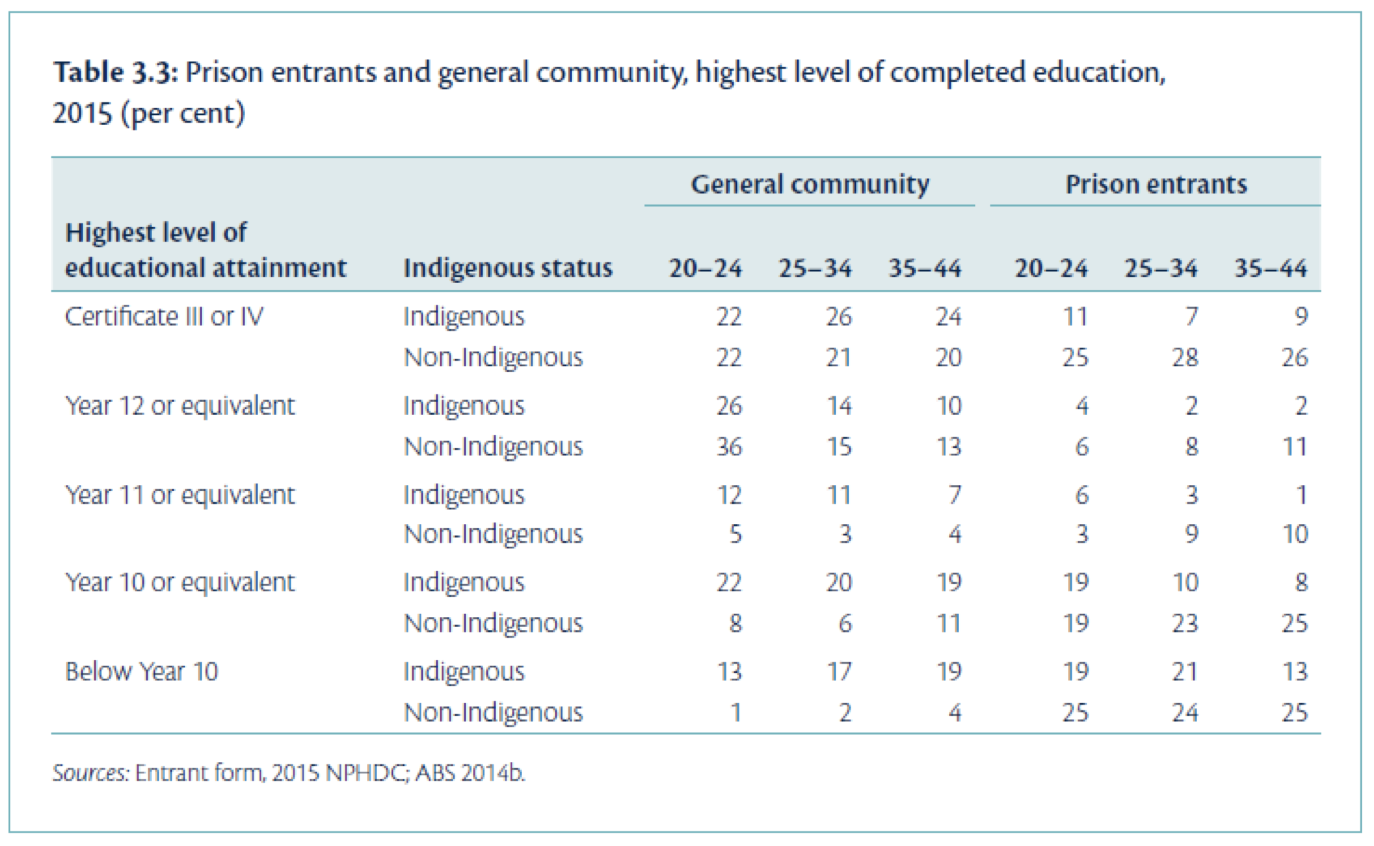
\includegraphics[width=0.66\textwidth,height=\textheight]{img/mod01/prisoner-education.png}

}

\caption{\label{fig-prison-education}Highest level of completed
education in prison entrants and the general community}

\end{figure}

Source: Australian Institute of Health and Welfare 2015. The health of
Australia's prisoners 2015. Cat. no. PHE 207. Canberra: AIHW.

Some issues in this table:

\begin{itemize}
\tightlist
\item
  The title of the table does not contain full information about the
  variables in the table;
\item
  It is unclear how the percentages were calculated (which groupings
  added to 100\%);
\item
  The ages are not labelled as such, thus without reading the text in
  report it is unclear that these are age groupings.
\end{itemize}

\hypertarget{summarising-two-categorical-variables-graphically}{%
\subsection{Summarising two categorical variables
graphically}\label{summarising-two-categorical-variables-graphically}}

Information from more than one variable can be presented as clustered or
multiple bar chart (bars side-by-side) (Figure~\ref{fig-bar-2}). This
type of graph is useful when examining changes in the categories
separately, but also comparing the grouping variable between the main
bar variable. Here we can see that Stage 3 and Stage 4 disease is the
most common for both males and females, but there are many more females
within each stage of disease.

\begin{figure}[H]

{\centering 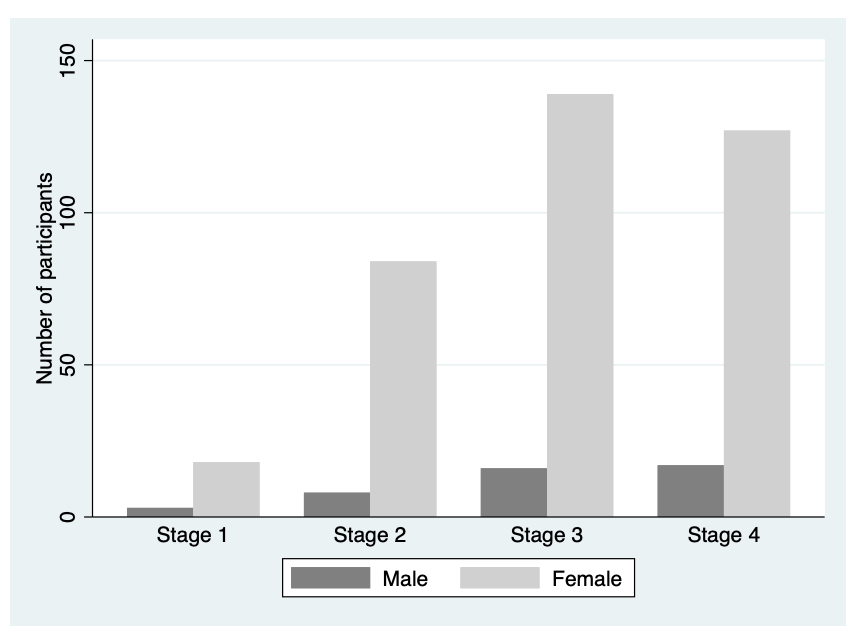
\includegraphics[width=0.75\textwidth,height=\textheight]{img/mod01/pbc-bar-stage-sex.png}

}

\caption{\label{fig-bar-2}Bar graph of stage of disease by sex from PBC
study}

\end{figure}

An alternative bar graph is a stacked or composite bar graph, which
retains the overall height for each category, but differentiates the
bars by another variable (Figure~\ref{fig-bar-3}).

\begin{figure}[H]

{\centering 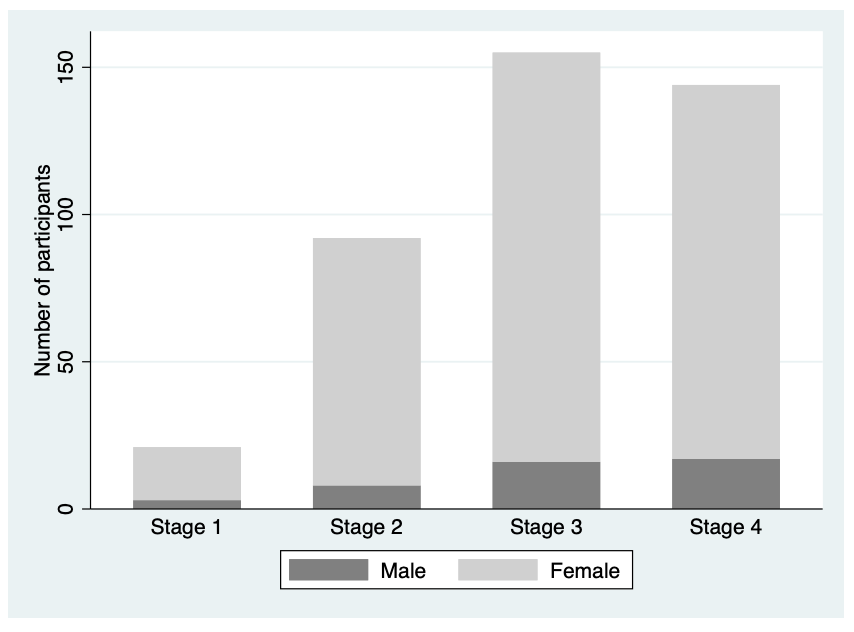
\includegraphics[width=0.75\textwidth,height=\textheight]{img/mod01/pbc-bar-stage-sex-stacked.png}

}

\caption{\label{fig-bar-3}Stacked bar graph of stage of disease by sex
from PBC study}

\end{figure}

Finally, a stacked relative bar chart (Figure~\ref{fig-bar-4}) displays
the proportion of grouping variable for each bar, where each overall bar
represents 100\%. These graphs allow the reader to compare the
proportions between categories. We can easily see from
Figure~\ref{fig-bar-4} that the distribution of sex is similar across
each stage of disease.

\begin{figure}[H]

{\centering 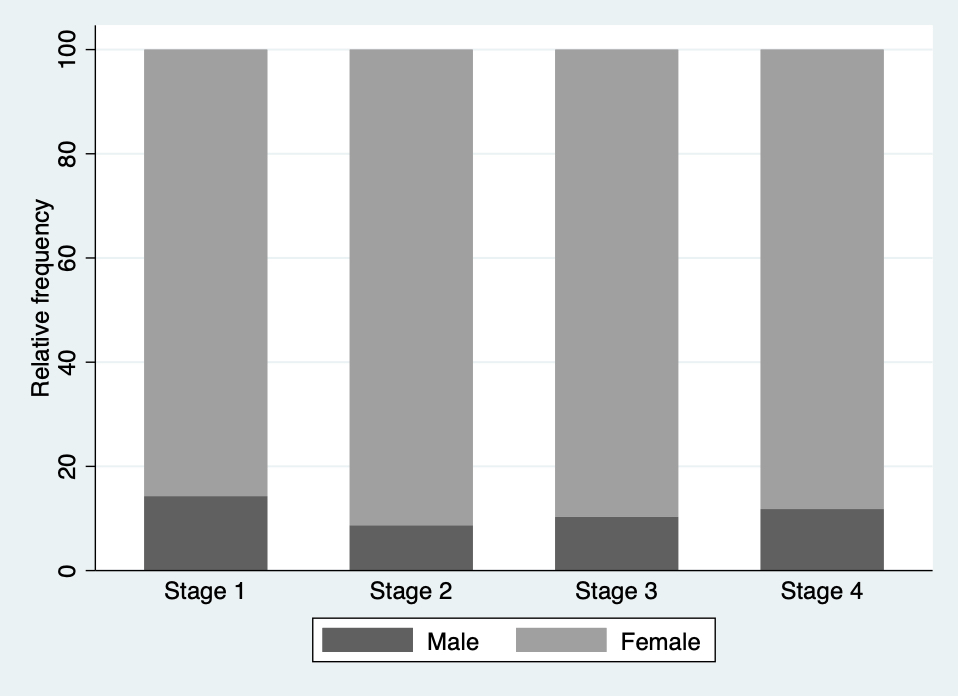
\includegraphics[width=0.75\textwidth,height=\textheight]{img/mod01/pbc-bar-stage-sex-stacked-relative.jpg}

}

\caption{\label{fig-bar-4}Relative frequency of sex within stage of
disease from PBC study}

\end{figure}

\hypertarget{presentation-guidelines}{%
\section{Presentation guidelines}\label{presentation-guidelines}}

\hypertarget{guidelines-for-presenting-summary-statistics}{%
\subsection{Guidelines for presenting summary
statistics}\label{guidelines-for-presenting-summary-statistics}}

When reporting summary statistics, it is important not to present
results with too many decimal places. Doing so implies that your data
have a higher level of precision than they do. For example, presenting a
mean blood pressure of 100.2487 mmHg implies that blood pressure can be
measured accurately to at least three decimal places.

There are a number of guidelines that have been written to help in the
presentation of numerical data. Many of these guidelines are based on
the number of decimal places, while others are based on the number of
significant figures. Briefly, the number of significant figures are
``the number of digits from the first non-zero digit to the last
meaningful digit, irrespective of the position of the decimal point.
Thus, 1.002, 10.02, 100200 (if this number is expressed to the nearest
100) all have four significant digits.'' Armitage, Berry, and Matthews
(2013)

A summary of these guidelines that will be used in this course appear in
Table~\ref{tbl-1-pres}.

\hypertarget{tbl-1-pres}{}
\global\setlength{\Oldarrayrulewidth}{\arrayrulewidth}

\global\setlength{\Oldtabcolsep}{\tabcolsep}

\setlength{\tabcolsep}{2pt}

\renewcommand*{\arraystretch}{1.5}



\providecommand{\ascline}[3]{\noalign{\global\arrayrulewidth #1}\arrayrulecolor[HTML]{#2}\cline{#3}}

\begin{longtable}[c]{|p{0.75in}|p{0.75in}}
\caption{\label{tbl-1-pres}Guidelines for presentation of statistical results }\tabularnewline




\ascline{1.5pt}{666666}{1-2}

\multicolumn{1}{>{\raggedright}m{\dimexpr 0.75in+0\tabcolsep}}{\textcolor[HTML]{000000}{\fontsize{11}{11}\selectfont{\global\setmainfont{Helvetica}{Summary\ statistic}}}} & \multicolumn{1}{>{\raggedright}m{\dimexpr 0.75in+0\tabcolsep}}{\textcolor[HTML]{000000}{\fontsize{11}{11}\selectfont{\global\setmainfont{Helvetica}{Guideline\ (reference)}}}} \\

\ascline{1.5pt}{666666}{1-2}\endfirsthead 

\ascline{1.5pt}{666666}{1-2}

\multicolumn{1}{>{\raggedright}m{\dimexpr 0.75in+0\tabcolsep}}{\textcolor[HTML]{000000}{\fontsize{11}{11}\selectfont{\global\setmainfont{Helvetica}{Summary\ statistic}}}} & \multicolumn{1}{>{\raggedright}m{\dimexpr 0.75in+0\tabcolsep}}{\textcolor[HTML]{000000}{\fontsize{11}{11}\selectfont{\global\setmainfont{Helvetica}{Guideline\ (reference)}}}} \\

\ascline{1.5pt}{666666}{1-2}\endhead



\multicolumn{1}{>{\raggedright}m{\dimexpr 0.75in+0\tabcolsep}}{\textcolor[HTML]{000000}{\fontsize{11}{11}\selectfont{\global\setmainfont{Helvetica}{Mean}}}} & \multicolumn{1}{>{\raggedright}m{\dimexpr 0.75in+0\tabcolsep}}{\textcolor[HTML]{000000}{\fontsize{11}{11}\selectfont{\global\setmainfont{Helvetica}{It\ is\ usually\ appropriate\ to\ quote\ the\ mean\ to\ one\ extra\ decimal\ place\ compared\ with\ the\ raw\ data.\ (Altman)}}}} \\





\multicolumn{1}{>{\raggedright}m{\dimexpr 0.75in+0\tabcolsep}}{\textcolor[HTML]{000000}{\fontsize{11}{11}\selectfont{\global\setmainfont{Helvetica}{Median,\ Interquartile\ range,\ Range}}}} & \multicolumn{1}{>{\raggedright}m{\dimexpr 0.75in+0\tabcolsep}}{\textcolor[HTML]{000000}{\fontsize{11}{11}\selectfont{\global\setmainfont{Helvetica}{As\ medians,\ interquartile\ ranges\ and\ ranges\ are\ based\ on\ individual\ data\ points,\ these\ values\ should\ be\ presented\ with\ the\ same\ precision\ as\ the\ original\ data.}}}} \\





\multicolumn{1}{>{\raggedright}m{\dimexpr 0.75in+0\tabcolsep}}{\textcolor[HTML]{000000}{\fontsize{11}{11}\selectfont{\global\setmainfont{Helvetica}{Percentage}}}} & \multicolumn{1}{>{\raggedright}m{\dimexpr 0.75in+0\tabcolsep}}{\textcolor[HTML]{000000}{\fontsize{11}{11}\selectfont{\global\setmainfont{Helvetica}{Percentages\ do\ not\ need\ to\ be\ given\ with\ more\ than\ one\ decimal\ place\ at\ most.\ When\ the\ sample\ size\ is\ less\ than\ 100,\ no\ decimal\ places\ should\ be\ given.\ (Altman)}}}} \\





\multicolumn{1}{>{\raggedright}m{\dimexpr 0.75in+0\tabcolsep}}{\textcolor[HTML]{000000}{\fontsize{11}{11}\selectfont{\global\setmainfont{Helvetica}{Probability}}}} & \multicolumn{1}{>{\raggedright}m{\dimexpr 0.75in+0\tabcolsep}}{\textcolor[HTML]{000000}{\fontsize{11}{11}\selectfont{\global\setmainfont{Helvetica}{It\ is\ acceptable\ to\ present\ probabilities\ to\ 2\ or\ 3\ decimal\ places.\ If\ the\ probability\ is\ presented\ as\ a\ percentage,\ present\ the\ percentage\ with\ 0\ or\ 1\ decimal\ place.}}}} \\





\multicolumn{1}{>{\raggedright}m{\dimexpr 0.75in+0\tabcolsep}}{\textcolor[HTML]{000000}{\fontsize{11}{11}\selectfont{\global\setmainfont{Helvetica}{Standard\ deviation}}}} & \multicolumn{1}{>{\raggedright}m{\dimexpr 0.75in+0\tabcolsep}}{\textcolor[HTML]{000000}{\fontsize{11}{11}\selectfont{\global\setmainfont{Helvetica}{The\ standard\ deviation\ should\ usually\ be\ given\ to\ the\ same\ accuracy\ as\ the\ mean,\ or\ with\ one\ extra\ decimal\ place.\ (Altman)}}}} \\





\multicolumn{1}{>{\raggedright}m{\dimexpr 0.75in+0\tabcolsep}}{\textcolor[HTML]{000000}{\fontsize{11}{11}\selectfont{\global\setmainfont{Helvetica}{Standard\ error}}}} & \multicolumn{1}{>{\raggedright}m{\dimexpr 0.75in+0\tabcolsep}}{\textcolor[HTML]{000000}{\fontsize{11}{11}\selectfont{\global\setmainfont{Helvetica}{As\ per\ standard\ deviation}}}} \\





\multicolumn{1}{>{\raggedright}m{\dimexpr 0.75in+0\tabcolsep}}{\textcolor[HTML]{000000}{\fontsize{11}{11}\selectfont{\global\setmainfont{Helvetica}{Confidence\ interval}}}} & \multicolumn{1}{>{\raggedright}m{\dimexpr 0.75in+0\tabcolsep}}{\textcolor[HTML]{000000}{\fontsize{11}{11}\selectfont{\global\setmainfont{Helvetica}{Use\ the\ same\ rule\ as\ for\ the\ corresponding\ effect\ size\ (be\ it\ mean,\ percentage,\ mean\ difference,\ regression\ coefficient,\ correlation\ coefficient\ or\ risk\ ratio)\ (Cole)}}}} \\





\multicolumn{1}{>{\raggedright}m{\dimexpr 0.75in+0\tabcolsep}}{\textcolor[HTML]{000000}{\fontsize{11}{11}\selectfont{\global\setmainfont{Helvetica}{Test\ statistic}}}} & \multicolumn{1}{>{\raggedright}m{\dimexpr 0.75in+0\tabcolsep}}{\textcolor[HTML]{000000}{\fontsize{11}{11}\selectfont{\global\setmainfont{Helvetica}{Test\ statistics\ should\ not\ be\ presented\ with\ more\ than\ two\ decimal\ places.}}}} \\





\multicolumn{1}{>{\raggedright}m{\dimexpr 0.75in+0\tabcolsep}}{\textcolor[HTML]{000000}{\fontsize{11}{11}\selectfont{\global\setmainfont{Helvetica}{P-value}}}} & \multicolumn{1}{>{\raggedright}m{\dimexpr 0.75in+0\tabcolsep}}{\textcolor[HTML]{000000}{\fontsize{11}{11}\selectfont{\global\setmainfont{Helvetica}{Report\ P-values\ to\ a\ single\ significant\ figure\ unless\ the\ P-value\ is\ close\ to\ 0.05\ (say,\ 0.01\ to\ 0.2),\ in\ which\ case,\ report\ two\ significant\ figures.\ Do\ not\ report\ `not\ significant`\ for\ P-values\ of\ 0.05\ or\ higher.\ Very\ low\ P-values\ can\ be\ reported\ as\ P\ <\ 0.001\ or\ P\ <\ 0.0001.\ A\ P-value\ can\ indeed\ be\ 1,\ although\ some\ investigators\ prefer\ to\ report\ this\ as\ >0.9.\ (Based\ on\ Assel)}}}} \\





\multicolumn{1}{>{\raggedright}m{\dimexpr 0.75in+0\tabcolsep}}{\textcolor[HTML]{000000}{\fontsize{11}{11}\selectfont{\global\setmainfont{Helvetica}{Difference\ in\ means}}}} & \multicolumn{1}{>{\raggedright}m{\dimexpr 0.75in+0\tabcolsep}}{\textcolor[HTML]{000000}{\fontsize{11}{11}\selectfont{\global\setmainfont{Helvetica}{As\ for\ the\ estimated\ means}}}} \\





\multicolumn{1}{>{\raggedright}m{\dimexpr 0.75in+0\tabcolsep}}{\textcolor[HTML]{000000}{\fontsize{11}{11}\selectfont{\global\setmainfont{Helvetica}{Difference\ in\ proportions}}}} & \multicolumn{1}{>{\raggedright}m{\dimexpr 0.75in+0\tabcolsep}}{\textcolor[HTML]{000000}{\fontsize{11}{11}\selectfont{\global\setmainfont{Helvetica}{As\ for\ the\ estimated\ proportions}}}} \\





\multicolumn{1}{>{\raggedright}m{\dimexpr 0.75in+0\tabcolsep}}{\textcolor[HTML]{000000}{\fontsize{11}{11}\selectfont{\global\setmainfont{Helvetica}{Odds\ ratio\ /\ Relative\ risk}}}} & \multicolumn{1}{>{\raggedright}m{\dimexpr 0.75in+0\tabcolsep}}{\textcolor[HTML]{000000}{\fontsize{11}{11}\selectfont{\global\setmainfont{Helvetica}{Hazard\ and\ odds\ ratios\ are\ normally\ reported\ to\ two\ decimal\ places,\ although\ this\ can\ be\ avoided\ for\ high\ odds\ ratios\ (Assel)}}}} \\





\multicolumn{1}{>{\raggedright}m{\dimexpr 0.75in+0\tabcolsep}}{\textcolor[HTML]{000000}{\fontsize{11}{11}\selectfont{\global\setmainfont{Helvetica}{Correlation\ coefficient}}}} & \multicolumn{1}{>{\raggedright}m{\dimexpr 0.75in+0\tabcolsep}}{\textcolor[HTML]{000000}{\fontsize{11}{11}\selectfont{\global\setmainfont{Helvetica}{One\ or\ two\ decimal\ places,\ or\ more\ when\ very\ close\ to\ ±1\ \ \ (Cole)}}}} \\





\multicolumn{1}{>{\raggedright}m{\dimexpr 0.75in+0\tabcolsep}}{\textcolor[HTML]{000000}{\fontsize{11}{11}\selectfont{\global\setmainfont{Helvetica}{Regression\ coefficient}}}} & \multicolumn{1}{>{\raggedright}m{\dimexpr 0.75in+0\tabcolsep}}{\textcolor[HTML]{000000}{\fontsize{11}{11}\selectfont{\global\setmainfont{Helvetica}{Use\ one\ more\ significant\ figure\ than\ the\ underlying\ data\ \ \ (adapted\ from\ Cole)}}}} \\

\ascline{1.5pt}{666666}{1-2}



\end{longtable}



\arrayrulecolor[HTML]{000000}

\global\setlength{\arrayrulewidth}{\Oldarrayrulewidth}

\global\setlength{\tabcolsep}{\Oldtabcolsep}

\renewcommand*{\arraystretch}{1}

\hypertarget{table-presentation-guidelines}{%
\subsection{Table presentation
guidelines}\label{table-presentation-guidelines}}

Consider the following guidelines for the appropriate presentation of
tables in scientific journals and reports (Woodward, 2013).

\begin{enumerate}
\def\labelenumi{\arabic{enumi}.}
\tightlist
\item
  Each table (and figure) should be self-explanatory, i.e.~the reader
  should be able to understand it without reference to the text in the
  body of the report.

  \begin{itemize}
  \tightlist
  \item
    This can be achieved by using complete, meaningful labels for the
    rows and columns and giving a complete, meaningful title.
  \item
    Footnotes can be used to enhance the explanation.
  \end{itemize}
\item
  Units of the variables (and if needed, method of calculation or
  derivation) should be given and missing records should be noted
  (e.g.~in a footnote).
\item
  A table should be visually uncluttered.

  \begin{itemize}
  \tightlist
  \item
    Avoid use of vertical lines.
  \item
    Horizontal lines should not be used in every single row, but they
    can be used to group parts of the table.
  \item
    Sensible use of white space also helps enormously; use equal spacing
    except where large spaces are left to separate distinct parts of the
    table.
  \item
    Different typefaces (or fonts) may be used to provide
    discrimination, e.g.~use of bold type and/or italics.
  \end{itemize}
\item
  The rows and columns of each table should be arranged in a natural
  order to help interpretation. For instance, when rows are ordered by
  the size of the numbers they contain for a nominal variable, it is
  immediately obvious where relatively big and small contributions come
  from.
\item
  Tables should have a consistent appearance throughout the report so
  that the paper is easy to follow (and also for an aesthetic
  appearance). Conventions for labelling and ordering should be the same
  (for both tables as well as figures) for ease of comparison of
  different tables (and figures).
\item
  Consider if there is a particular table orientation that makes a table
  easier to read.
\end{enumerate}

Given the different possible formats of tables and their complexity,
some further guidelines are given in the following excellent references:

\begin{itemize}
\tightlist
\item
  Graphics and statistics for cardiology: designing effective tables for
  presentation and publication, Boers (2018)
\item
  Guidelines for Reporting of Figures and Tables for Clinical Research
  in Urology, Vickers et al. (2020)
\end{itemize}

\hypertarget{graphical-presentation-guidelines}{%
\subsection{Graphical presentation
guidelines}\label{graphical-presentation-guidelines}}

Consider the following guidelines for the appropriate presentation of
graphs in scientific journals and reports (Woodward, 2013).

\begin{itemize}
\tightlist
\item
  Figures should be self-explanatory and have consistent appearance
  through the report.
\item
  A title should give complete information. Note that figure titles are
  usually placed below the figure, whereas for tables titles are given
  above the table.
\item
  Axes should be labelled appropriately
\item
  Units of the variables should be given in the labelling of the axes.
  Use footnotes to indicate any calculation or derivation of variables
  and to indicate missing values
\item
  If the Y-axis has a natural origin, it should be included, or
  emphasised if it is not included.
\item
  If graphs are being compared, the Y-axis should be the same across the
  graphs to enable fair comparison
\item
  Columns of bar charts should be separated by a space
\item
  Three dimensional graphs should be avoided unless the third dimension
  adds additional information
\end{itemize}

Sources:

Altman (1990)

Cole (2015)

Assel et al. (2019)

\hypertarget{probability}{%
\section{Probability}\label{probability}}

Probability is defined as:

\begin{quote}
the chance of an event occurring, where an event is the result of an
observation or experiment, or the description of some potential outcome.
\end{quote}

Probabilities range from 0 (where the event will never occur) to 1
(where the event will always occur). For example, tossing a coin is an
experiment; one event is the coin landing with head up, while the other
event is the coin landing tails up. The set of all possible outcomes in
an experiment is called the sample space. For example, by tossing a coin
you can get either a head or a tail (called mutually exclusive events);
and by rolling a die you can get any of the six sides. Thus, for a die
the sampling space is: S = \{1, 2, 3, 4, 5, 6\}

With a fair (unbiased) die, the probability of each outcome occurring is
1/6 and its probability distribution is simply a probability of 1/6 for
each of the six numbers on a die.

\hypertarget{additive-law-of-probability}{%
\subsection{Additive law of
probability}\label{additive-law-of-probability}}

How do we work out the probability that one roll of a die will turn out
to be a 3 or a 6? To do that, we first need to work out whether the
events (3 or 6 on the roll of a die) are mutually exclusive. Events are
mutually exclusive if they are events which cannot occur at the same
time. For example, rolling a die once and getting a 3 and 6 are mutually
exclusive events (you can roll one or the other but not both in a single
roll).

To obtain the probability of one or the other of two mutually exclusive
events occurring, the sum of the probabilities of each is taken. For
example, the probability of the roll of a die being a 3 or a 6 is the
sum of the probability of the die being 3 (i.e.~1/6) and the probability
of the die being 6 (also 1/6). With a fair die:

Probability of a die roll being 3 or 6 = \(1/6 + 1/6 = 1/3\)

Another way of putting it is:

P(die roll =3 or die roll =6) = P(die roll=3) + P(die roll=6) =
\(1/6 + 1/6 = 1/3\)

\hypertarget{example-additive-law-for-mutually-exclusive-events}{%
\subsubsection*{Example: Additive law for mutually exclusive
events}\label{example-additive-law-for-mutually-exclusive-events}}
\addcontentsline{toc}{subsubsection}{Example: Additive law for mutually
exclusive events}

Consider that blood type can be organised into the ABO system (blood
types A, B, AB or O) An individual may only have one blood type.

Using the information from
https://www.donateblood.com.au/learn/about-blood let's consider the ABO
blood type system. The frequency distribution (prevalence) of the ABO
blood type system in the population represents the probability of each
of the outcomes. If we consider all possible blood type outcomes, then
the total of the probabilities will sum to 1 (100\%).

\hypertarget{tbl-2-1}{}
\global\setlength{\Oldarrayrulewidth}{\arrayrulewidth}

\global\setlength{\Oldtabcolsep}{\tabcolsep}

\setlength{\tabcolsep}{2pt}

\renewcommand*{\arraystretch}{1.5}



\providecommand{\ascline}[3]{\noalign{\global\arrayrulewidth #1}\arrayrulecolor[HTML]{#2}\cline{#3}}

\begin{longtable}[c]{|p{0.75in}|p{0.75in}|p{0.75in}}
\caption{\label{tbl-2-1}Frequency of blood types }\tabularnewline




\ascline{1.5pt}{666666}{1-3}

\multicolumn{1}{>{\raggedright}m{\dimexpr 0.75in+0\tabcolsep}}{\textcolor[HTML]{000000}{\fontsize{11}{11}\selectfont{\global\setmainfont{Helvetica}{Blood\ Type}}}} & \multicolumn{1}{>{\raggedright}m{\dimexpr 0.75in+0\tabcolsep}}{\textcolor[HTML]{000000}{\fontsize{11}{11}\selectfont{\global\setmainfont{Helvetica}{\%\ of\ population}}}} & \multicolumn{1}{>{\raggedleft}m{\dimexpr 0.75in+0\tabcolsep}}{\textcolor[HTML]{000000}{\fontsize{11}{11}\selectfont{\global\setmainfont{Helvetica}{Probability}}}} \\

\ascline{1.5pt}{666666}{1-3}\endfirsthead 

\ascline{1.5pt}{666666}{1-3}

\multicolumn{1}{>{\raggedright}m{\dimexpr 0.75in+0\tabcolsep}}{\textcolor[HTML]{000000}{\fontsize{11}{11}\selectfont{\global\setmainfont{Helvetica}{Blood\ Type}}}} & \multicolumn{1}{>{\raggedright}m{\dimexpr 0.75in+0\tabcolsep}}{\textcolor[HTML]{000000}{\fontsize{11}{11}\selectfont{\global\setmainfont{Helvetica}{\%\ of\ population}}}} & \multicolumn{1}{>{\raggedleft}m{\dimexpr 0.75in+0\tabcolsep}}{\textcolor[HTML]{000000}{\fontsize{11}{11}\selectfont{\global\setmainfont{Helvetica}{Probability}}}} \\

\ascline{1.5pt}{666666}{1-3}\endhead



\multicolumn{1}{>{\raggedright}m{\dimexpr 0.75in+0\tabcolsep}}{\textcolor[HTML]{000000}{\fontsize{11}{11}\selectfont{\global\setmainfont{Helvetica}{A}}}} & \multicolumn{1}{>{\raggedright}m{\dimexpr 0.75in+0\tabcolsep}}{\textcolor[HTML]{000000}{\fontsize{11}{11}\selectfont{\global\setmainfont{Helvetica}{38\%}}}} & \multicolumn{1}{>{\raggedleft}m{\dimexpr 0.75in+0\tabcolsep}}{\textcolor[HTML]{000000}{\fontsize{11}{11}\selectfont{\global\setmainfont{Helvetica}{0.38}}}} \\





\multicolumn{1}{>{\raggedright}m{\dimexpr 0.75in+0\tabcolsep}}{\textcolor[HTML]{000000}{\fontsize{11}{11}\selectfont{\global\setmainfont{Helvetica}{B}}}} & \multicolumn{1}{>{\raggedright}m{\dimexpr 0.75in+0\tabcolsep}}{\textcolor[HTML]{000000}{\fontsize{11}{11}\selectfont{\global\setmainfont{Helvetica}{10\%}}}} & \multicolumn{1}{>{\raggedleft}m{\dimexpr 0.75in+0\tabcolsep}}{\textcolor[HTML]{000000}{\fontsize{11}{11}\selectfont{\global\setmainfont{Helvetica}{0.10}}}} \\





\multicolumn{1}{>{\raggedright}m{\dimexpr 0.75in+0\tabcolsep}}{\textcolor[HTML]{000000}{\fontsize{11}{11}\selectfont{\global\setmainfont{Helvetica}{AB}}}} & \multicolumn{1}{>{\raggedright}m{\dimexpr 0.75in+0\tabcolsep}}{\textcolor[HTML]{000000}{\fontsize{11}{11}\selectfont{\global\setmainfont{Helvetica}{3\%}}}} & \multicolumn{1}{>{\raggedleft}m{\dimexpr 0.75in+0\tabcolsep}}{\textcolor[HTML]{000000}{\fontsize{11}{11}\selectfont{\global\setmainfont{Helvetica}{0.03}}}} \\





\multicolumn{1}{>{\raggedright}m{\dimexpr 0.75in+0\tabcolsep}}{\textcolor[HTML]{000000}{\fontsize{11}{11}\selectfont{\global\setmainfont{Helvetica}{O}}}} & \multicolumn{1}{>{\raggedright}m{\dimexpr 0.75in+0\tabcolsep}}{\textcolor[HTML]{000000}{\fontsize{11}{11}\selectfont{\global\setmainfont{Helvetica}{49\%}}}} & \multicolumn{1}{>{\raggedleft}m{\dimexpr 0.75in+0\tabcolsep}}{\textcolor[HTML]{000000}{\fontsize{11}{11}\selectfont{\global\setmainfont{Helvetica}{0.49}}}} \\





\multicolumn{1}{>{\raggedright}m{\dimexpr 0.75in+0\tabcolsep}}{\textcolor[HTML]{000000}{\fontsize{11}{11}\selectfont{\global\setmainfont{Helvetica}{Total}}}} & \multicolumn{1}{>{\raggedright}m{\dimexpr 0.75in+0\tabcolsep}}{\textcolor[HTML]{000000}{\fontsize{11}{11}\selectfont{\global\setmainfont{Helvetica}{100\%}}}} & \multicolumn{1}{>{\raggedleft}m{\dimexpr 0.75in+0\tabcolsep}}{\textcolor[HTML]{000000}{\fontsize{11}{11}\selectfont{\global\setmainfont{Helvetica}{1.00}}}} \\

\ascline{1.5pt}{666666}{1-3}



\end{longtable}



\arrayrulecolor[HTML]{000000}

\global\setlength{\arrayrulewidth}{\Oldarrayrulewidth}

\global\setlength{\tabcolsep}{\Oldtabcolsep}

\renewcommand*{\arraystretch}{1}

In this example we consider: What is the probability that an individual
will have either blood group O or A?

Since blood type is mutually exclusive, the probability that either one
or the other occurs is the sum of the individual probabilities. These
are mutually exclusive events so we can say P(O or A) = P(O) + P(A)

Thus, the answer is: P(Blood type O) + P(Blood type A) = 0.49 + 0.38 =
0.87

\hypertarget{multiplicative-law-of-probability}{%
\subsection{Multiplicative law of
probability}\label{multiplicative-law-of-probability}}

The additive law of probability lets us consider the probability of
different outcomes in a single experiment. The multiplicative law lets
us consider the probability of multiple events occurring in a particular
order. For example: if I roll a die twice, what is the probability of
rolling a 3 and \emph{then} a 6?

These events are independent: the probability of rolling a 6 on the
second roll is not affected by the first roll.

The multiplicative law of probability states:

\begin{quote}
If A and B are independent, then P(A and B) = P(A) \(\times\) P(B).
\end{quote}

So, the probability of rolling a 3 and then a 6 is: P(3 and 6) =
\(1/6 \times 1/6 = 1/36\).

Note here that the order matters -- we are considering the probability
of rolling a 3 and then a 6, not the probability of rolling a 6 and then
a 3.

\hypertarget{probability-distributions}{%
\section{Probability distributions}\label{probability-distributions}}

\begin{quote}
A probability distribution is a table or a function that provides the
probabilities of all possible outcomes for a random event.
\end{quote}

For example, the probability distribution for a single coin toss is
straightforward: the probability of obtaining a head is 0.5, and the
probability of obtaining a tail is 0.5, and this can be summarised in
Table~\ref{tbl-coin}.

\hypertarget{tbl-coin}{}
\global\setlength{\Oldarrayrulewidth}{\arrayrulewidth}

\global\setlength{\Oldtabcolsep}{\tabcolsep}

\setlength{\tabcolsep}{2pt}

\renewcommand*{\arraystretch}{1.5}



\providecommand{\ascline}[3]{\noalign{\global\arrayrulewidth #1}\arrayrulecolor[HTML]{#2}\cline{#3}}

\begin{longtable}[c]{|p{0.75in}|p{0.75in}}
\caption{\label{tbl-coin}Probability distribution for a single coin toss }\tabularnewline




\ascline{1.5pt}{666666}{1-2}

\multicolumn{1}{>{\raggedright}m{\dimexpr 0.75in+0\tabcolsep}}{\textcolor[HTML]{000000}{\fontsize{11}{11}\selectfont{\global\setmainfont{Helvetica}{Coin\ face}}}} & \multicolumn{1}{>{\raggedleft}m{\dimexpr 0.75in+0\tabcolsep}}{\textcolor[HTML]{000000}{\fontsize{11}{11}\selectfont{\global\setmainfont{Helvetica}{Probability}}}} \\

\ascline{1.5pt}{666666}{1-2}\endfirsthead 

\ascline{1.5pt}{666666}{1-2}

\multicolumn{1}{>{\raggedright}m{\dimexpr 0.75in+0\tabcolsep}}{\textcolor[HTML]{000000}{\fontsize{11}{11}\selectfont{\global\setmainfont{Helvetica}{Coin\ face}}}} & \multicolumn{1}{>{\raggedleft}m{\dimexpr 0.75in+0\tabcolsep}}{\textcolor[HTML]{000000}{\fontsize{11}{11}\selectfont{\global\setmainfont{Helvetica}{Probability}}}} \\

\ascline{1.5pt}{666666}{1-2}\endhead



\multicolumn{1}{>{\raggedright}m{\dimexpr 0.75in+0\tabcolsep}}{\textcolor[HTML]{000000}{\fontsize{11}{11}\selectfont{\global\setmainfont{Helvetica}{Heads}}}} & \multicolumn{1}{>{\raggedleft}m{\dimexpr 0.75in+0\tabcolsep}}{\textcolor[HTML]{000000}{\fontsize{11}{11}\selectfont{\global\setmainfont{Helvetica}{0.5}}}} \\





\multicolumn{1}{>{\raggedright}m{\dimexpr 0.75in+0\tabcolsep}}{\textcolor[HTML]{000000}{\fontsize{11}{11}\selectfont{\global\setmainfont{Helvetica}{Tails}}}} & \multicolumn{1}{>{\raggedleft}m{\dimexpr 0.75in+0\tabcolsep}}{\textcolor[HTML]{000000}{\fontsize{11}{11}\selectfont{\global\setmainfont{Helvetica}{0.5}}}} \\

\ascline{1.5pt}{666666}{1-2}



\end{longtable}



\arrayrulecolor[HTML]{000000}

\global\setlength{\arrayrulewidth}{\Oldarrayrulewidth}

\global\setlength{\tabcolsep}{\Oldtabcolsep}

\renewcommand*{\arraystretch}{1}

Similarly, the probability distribution for a single roll of a die is
straightforward: each face has a probability of 1/6
(Table~\ref{tbl-die}).

\hypertarget{tbl-die}{}
\global\setlength{\Oldarrayrulewidth}{\arrayrulewidth}

\global\setlength{\Oldtabcolsep}{\tabcolsep}

\setlength{\tabcolsep}{2pt}

\renewcommand*{\arraystretch}{1.5}



\providecommand{\ascline}[3]{\noalign{\global\arrayrulewidth #1}\arrayrulecolor[HTML]{#2}\cline{#3}}

\begin{longtable}[c]{|p{0.75in}|p{0.75in}}
\caption{\label{tbl-die}Probability distributions for a single roll of a die }\tabularnewline




\ascline{1.5pt}{666666}{1-2}

\multicolumn{1}{>{\raggedleft}m{\dimexpr 0.75in+0\tabcolsep}}{\textcolor[HTML]{000000}{\fontsize{11}{11}\selectfont{\global\setmainfont{Helvetica}{Face\ of\ a\ die}}}} & \multicolumn{1}{>{\raggedright}m{\dimexpr 0.75in+0\tabcolsep}}{\textcolor[HTML]{000000}{\fontsize{11}{11}\selectfont{\global\setmainfont{Helvetica}{Probability}}}} \\

\ascline{1.5pt}{666666}{1-2}\endfirsthead 

\ascline{1.5pt}{666666}{1-2}

\multicolumn{1}{>{\raggedleft}m{\dimexpr 0.75in+0\tabcolsep}}{\textcolor[HTML]{000000}{\fontsize{11}{11}\selectfont{\global\setmainfont{Helvetica}{Face\ of\ a\ die}}}} & \multicolumn{1}{>{\raggedright}m{\dimexpr 0.75in+0\tabcolsep}}{\textcolor[HTML]{000000}{\fontsize{11}{11}\selectfont{\global\setmainfont{Helvetica}{Probability}}}} \\

\ascline{1.5pt}{666666}{1-2}\endhead



\multicolumn{1}{>{\raggedleft}m{\dimexpr 0.75in+0\tabcolsep}}{\textcolor[HTML]{000000}{\fontsize{11}{11}\selectfont{\global\setmainfont{Helvetica}{1}}}} & \multicolumn{1}{>{\raggedright}m{\dimexpr 0.75in+0\tabcolsep}}{\textcolor[HTML]{000000}{\fontsize{11}{11}\selectfont{\global\setmainfont{Helvetica}{1/6}}}} \\





\multicolumn{1}{>{\raggedleft}m{\dimexpr 0.75in+0\tabcolsep}}{\textcolor[HTML]{000000}{\fontsize{11}{11}\selectfont{\global\setmainfont{Helvetica}{2}}}} & \multicolumn{1}{>{\raggedright}m{\dimexpr 0.75in+0\tabcolsep}}{\textcolor[HTML]{000000}{\fontsize{11}{11}\selectfont{\global\setmainfont{Helvetica}{1/6}}}} \\





\multicolumn{1}{>{\raggedleft}m{\dimexpr 0.75in+0\tabcolsep}}{\textcolor[HTML]{000000}{\fontsize{11}{11}\selectfont{\global\setmainfont{Helvetica}{3}}}} & \multicolumn{1}{>{\raggedright}m{\dimexpr 0.75in+0\tabcolsep}}{\textcolor[HTML]{000000}{\fontsize{11}{11}\selectfont{\global\setmainfont{Helvetica}{1/6}}}} \\





\multicolumn{1}{>{\raggedleft}m{\dimexpr 0.75in+0\tabcolsep}}{\textcolor[HTML]{000000}{\fontsize{11}{11}\selectfont{\global\setmainfont{Helvetica}{4}}}} & \multicolumn{1}{>{\raggedright}m{\dimexpr 0.75in+0\tabcolsep}}{\textcolor[HTML]{000000}{\fontsize{11}{11}\selectfont{\global\setmainfont{Helvetica}{1/6}}}} \\





\multicolumn{1}{>{\raggedleft}m{\dimexpr 0.75in+0\tabcolsep}}{\textcolor[HTML]{000000}{\fontsize{11}{11}\selectfont{\global\setmainfont{Helvetica}{5}}}} & \multicolumn{1}{>{\raggedright}m{\dimexpr 0.75in+0\tabcolsep}}{\textcolor[HTML]{000000}{\fontsize{11}{11}\selectfont{\global\setmainfont{Helvetica}{1/6}}}} \\





\multicolumn{1}{>{\raggedleft}m{\dimexpr 0.75in+0\tabcolsep}}{\textcolor[HTML]{000000}{\fontsize{11}{11}\selectfont{\global\setmainfont{Helvetica}{6}}}} & \multicolumn{1}{>{\raggedright}m{\dimexpr 0.75in+0\tabcolsep}}{\textcolor[HTML]{000000}{\fontsize{11}{11}\selectfont{\global\setmainfont{Helvetica}{1/6}}}} \\

\ascline{1.5pt}{666666}{1-2}



\end{longtable}



\arrayrulecolor[HTML]{000000}

\global\setlength{\arrayrulewidth}{\Oldarrayrulewidth}

\global\setlength{\tabcolsep}{\Oldtabcolsep}

\renewcommand*{\arraystretch}{1}

Things become more complicated when we consider multiple coin-tosses, or
rolls of a die. These series of events can be summarised by considering
the number of times a certain outcome is observed. For example, the
probability of obtaining three heads from five coin tosses.

Probability distributions can be used in two main ways:

\begin{enumerate}
\def\labelenumi{\arabic{enumi}.}
\tightlist
\item
  To calculate the probability of an event occurring. This seems trivial
  for the coin-toss and die-roll examples above. However, we can
  consider more complex events, as below.
\item
  To understand the behaviour of a sample statistic. We will see in
  Modules 3 and 4 that we can assume the mean of a sample follows a
  probability distribution. We can obtain useful information about the
  sample mean by using properties of the probability distribution.
\end{enumerate}

\hypertarget{discrete-random-variables-and-their-probability-distributions}{%
\section{Discrete random variables and their probability
distributions}\label{discrete-random-variables-and-their-probability-distributions}}

Rather than thinking of random events, we often use the term
\emph{random variable} to describe a quantity that can have different
values determined by chance.

A \emph{discrete random variable} is a random variable that can take on
only countable values (that is, non-negative whole numbers). An example
of a discrete random variable is the number of heads observed in a
series of coin tosses.

A discrete random variable can be summarised by listing all the possible
values that the variable can take. As defined earlier, a table, formula
or graph that presents these possible values, and their associated
probabilities, is called a probability distribution.

Example: let's consider the number of heads in a series of three coin
tosses. We might observe 0 heads, or 1 head, or 2, or 3 heads. If we let
X denote the number of heads in a series of three coin tosses, then
possible values of X are 0, 1, 2 or 3.

We write the probability of observing x heads as P(X=x). So P(X=0) is
the probability that the three tosses has no heads. Similarly, P(X=1) is
the probability of observing one head.

The possible combinations for three coin tosses are as follows:

\hypertarget{tbl-2-3toss}{}
\global\setlength{\Oldarrayrulewidth}{\arrayrulewidth}

\global\setlength{\Oldtabcolsep}{\tabcolsep}

\setlength{\tabcolsep}{2pt}

\renewcommand*{\arraystretch}{1.5}



\providecommand{\ascline}[3]{\noalign{\global\arrayrulewidth #1}\arrayrulecolor[HTML]{#2}\cline{#3}}

\begin{longtable}[c]{|p{0.75in}|p{0.75in}}
\caption{\label{tbl-2-3toss}The number of heads from three coin tosses }\tabularnewline




\ascline{1.5pt}{666666}{1-2}

\multicolumn{1}{>{\raggedright}m{\dimexpr 0.75in+0\tabcolsep}}{\textcolor[HTML]{000000}{\fontsize{11}{11}\selectfont{\global\setmainfont{Helvetica}{Pattern}}}} & \multicolumn{1}{>{\raggedleft}m{\dimexpr 0.75in+0\tabcolsep}}{\textcolor[HTML]{000000}{\fontsize{11}{11}\selectfont{\global\setmainfont{Helvetica}{Number\ of\ heads}}}} \\

\ascline{1.5pt}{666666}{1-2}\endfirsthead 

\ascline{1.5pt}{666666}{1-2}

\multicolumn{1}{>{\raggedright}m{\dimexpr 0.75in+0\tabcolsep}}{\textcolor[HTML]{000000}{\fontsize{11}{11}\selectfont{\global\setmainfont{Helvetica}{Pattern}}}} & \multicolumn{1}{>{\raggedleft}m{\dimexpr 0.75in+0\tabcolsep}}{\textcolor[HTML]{000000}{\fontsize{11}{11}\selectfont{\global\setmainfont{Helvetica}{Number\ of\ heads}}}} \\

\ascline{1.5pt}{666666}{1-2}\endhead



\multicolumn{1}{>{\raggedright}m{\dimexpr 0.75in+0\tabcolsep}}{\textcolor[HTML]{000000}{\fontsize{11}{11}\selectfont{\global\setmainfont{Helvetica}{Tail,\ Tail,\ Tail}}}} & \multicolumn{1}{>{\raggedleft}m{\dimexpr 0.75in+0\tabcolsep}}{\textcolor[HTML]{000000}{\fontsize{11}{11}\selectfont{\global\setmainfont{Helvetica}{0}}}} \\





\multicolumn{1}{>{\raggedright}m{\dimexpr 0.75in+0\tabcolsep}}{\textcolor[HTML]{000000}{\fontsize{11}{11}\selectfont{\global\setmainfont{Helvetica}{Head,\ Tail,\ Tail}}}} & \multicolumn{1}{>{\raggedleft}m{\dimexpr 0.75in+0\tabcolsep}}{\textcolor[HTML]{000000}{\fontsize{11}{11}\selectfont{\global\setmainfont{Helvetica}{}}}} \\





\multicolumn{1}{>{\raggedright}m{\dimexpr 0.75in+0\tabcolsep}}{\textcolor[HTML]{000000}{\fontsize{11}{11}\selectfont{\global\setmainfont{Helvetica}{Tail,\ Head,\ Tail}}}} & \multicolumn{1}{>{\raggedleft}m{\dimexpr 0.75in+0\tabcolsep}}{\textcolor[HTML]{000000}{\fontsize{11}{11}\selectfont{\global\setmainfont{Helvetica}{1}}}} \\





\multicolumn{1}{>{\raggedright}m{\dimexpr 0.75in+0\tabcolsep}}{\textcolor[HTML]{000000}{\fontsize{11}{11}\selectfont{\global\setmainfont{Helvetica}{Tail,\ Tail,\ Head}}}} & \multicolumn{1}{>{\raggedleft}m{\dimexpr 0.75in+0\tabcolsep}}{\textcolor[HTML]{000000}{\fontsize{11}{11}\selectfont{\global\setmainfont{Helvetica}{}}}} \\





\multicolumn{1}{>{\raggedright}m{\dimexpr 0.75in+0\tabcolsep}}{\textcolor[HTML]{000000}{\fontsize{11}{11}\selectfont{\global\setmainfont{Helvetica}{Head,\ Head,\ Tail}}}} & \multicolumn{1}{>{\raggedleft}m{\dimexpr 0.75in+0\tabcolsep}}{\textcolor[HTML]{000000}{\fontsize{11}{11}\selectfont{\global\setmainfont{Helvetica}{}}}} \\





\multicolumn{1}{>{\raggedright}m{\dimexpr 0.75in+0\tabcolsep}}{\textcolor[HTML]{000000}{\fontsize{11}{11}\selectfont{\global\setmainfont{Helvetica}{Head,\ Tail,\ Head}}}} & \multicolumn{1}{>{\raggedleft}m{\dimexpr 0.75in+0\tabcolsep}}{\textcolor[HTML]{000000}{\fontsize{11}{11}\selectfont{\global\setmainfont{Helvetica}{2}}}} \\





\multicolumn{1}{>{\raggedright}m{\dimexpr 0.75in+0\tabcolsep}}{\textcolor[HTML]{000000}{\fontsize{11}{11}\selectfont{\global\setmainfont{Helvetica}{Tail,\ Head,\ Head}}}} & \multicolumn{1}{>{\raggedleft}m{\dimexpr 0.75in+0\tabcolsep}}{\textcolor[HTML]{000000}{\fontsize{11}{11}\selectfont{\global\setmainfont{Helvetica}{}}}} \\





\multicolumn{1}{>{\raggedright}m{\dimexpr 0.75in+0\tabcolsep}}{\textcolor[HTML]{000000}{\fontsize{11}{11}\selectfont{\global\setmainfont{Helvetica}{Head,\ Head,\ Head}}}} & \multicolumn{1}{>{\raggedleft}m{\dimexpr 0.75in+0\tabcolsep}}{\textcolor[HTML]{000000}{\fontsize{11}{11}\selectfont{\global\setmainfont{Helvetica}{3}}}} \\

\ascline{1.5pt}{666666}{1-2}



\end{longtable}



\arrayrulecolor[HTML]{000000}

\global\setlength{\arrayrulewidth}{\Oldarrayrulewidth}

\global\setlength{\tabcolsep}{\Oldtabcolsep}

\renewcommand*{\arraystretch}{1}

There are eight possible outcomes from three coin tosses (permutations).
If we assume an equal chance of observing a head or a tail, each
permutation above is equally likely, and so has a probability of 1/8.

If we consider the possibility of observing just one head out of the
three tosses, this can happen in three ways (HTT, THT, TTH). So the
probability of observing one head is calculated using the additive law:
P(X=1) = \(\tfrac{1}{8} + \tfrac{1}{8} + \tfrac{1}{8} = \tfrac{3}{8}\).

Therefore, the probability distribution for X, the number of heads from
three coin tosses, is as follows:

\hypertarget{tbl-2-4}{}
\global\setlength{\Oldarrayrulewidth}{\arrayrulewidth}

\global\setlength{\Oldtabcolsep}{\tabcolsep}

\setlength{\tabcolsep}{2pt}

\renewcommand*{\arraystretch}{1.5}



\providecommand{\ascline}[3]{\noalign{\global\arrayrulewidth #1}\arrayrulecolor[HTML]{#2}\cline{#3}}

\begin{longtable}[c]{|p{0.75in}|p{0.75in}}
\caption{\label{tbl-2-4}Probability distribution for the number of heads from three coin tosses }\tabularnewline




\ascline{1.5pt}{666666}{1-2}

\multicolumn{1}{>{\raggedleft}m{\dimexpr 0.75in+0\tabcolsep}}{\textcolor[HTML]{000000}{\fontsize{11}{11}\selectfont{\global\setmainfont{Helvetica}{x\ (number\ of\ heads\ observed)}}}} & \multicolumn{1}{>{\raggedright}m{\dimexpr 0.75in+0\tabcolsep}}{\textcolor[HTML]{000000}{\fontsize{11}{11}\selectfont{\global\setmainfont{Helvetica}{P(X=x)}}}} \\

\ascline{1.5pt}{666666}{1-2}\endfirsthead 

\ascline{1.5pt}{666666}{1-2}

\multicolumn{1}{>{\raggedleft}m{\dimexpr 0.75in+0\tabcolsep}}{\textcolor[HTML]{000000}{\fontsize{11}{11}\selectfont{\global\setmainfont{Helvetica}{x\ (number\ of\ heads\ observed)}}}} & \multicolumn{1}{>{\raggedright}m{\dimexpr 0.75in+0\tabcolsep}}{\textcolor[HTML]{000000}{\fontsize{11}{11}\selectfont{\global\setmainfont{Helvetica}{P(X=x)}}}} \\

\ascline{1.5pt}{666666}{1-2}\endhead



\multicolumn{1}{>{\raggedleft}m{\dimexpr 0.75in+0\tabcolsep}}{\textcolor[HTML]{000000}{\fontsize{11}{11}\selectfont{\global\setmainfont{Helvetica}{0}}}} & \multicolumn{1}{>{\raggedright}m{\dimexpr 0.75in+0\tabcolsep}}{\textcolor[HTML]{000000}{\fontsize{11}{11}\selectfont{\global\setmainfont{Helvetica}{1/8}}}} \\





\multicolumn{1}{>{\raggedleft}m{\dimexpr 0.75in+0\tabcolsep}}{\textcolor[HTML]{000000}{\fontsize{11}{11}\selectfont{\global\setmainfont{Helvetica}{1}}}} & \multicolumn{1}{>{\raggedright}m{\dimexpr 0.75in+0\tabcolsep}}{\textcolor[HTML]{000000}{\fontsize{11}{11}\selectfont{\global\setmainfont{Helvetica}{1/8\ +\ 1/8\ +\ 1/8\ =\ 3/8}}}} \\





\multicolumn{1}{>{\raggedleft}m{\dimexpr 0.75in+0\tabcolsep}}{\textcolor[HTML]{000000}{\fontsize{11}{11}\selectfont{\global\setmainfont{Helvetica}{2}}}} & \multicolumn{1}{>{\raggedright}m{\dimexpr 0.75in+0\tabcolsep}}{\textcolor[HTML]{000000}{\fontsize{11}{11}\selectfont{\global\setmainfont{Helvetica}{1/8\ +\ 1/8\ +\ 1/8\ =\ 3/8}}}} \\





\multicolumn{1}{>{\raggedleft}m{\dimexpr 0.75in+0\tabcolsep}}{\textcolor[HTML]{000000}{\fontsize{11}{11}\selectfont{\global\setmainfont{Helvetica}{3}}}} & \multicolumn{1}{>{\raggedright}m{\dimexpr 0.75in+0\tabcolsep}}{\textcolor[HTML]{000000}{\fontsize{11}{11}\selectfont{\global\setmainfont{Helvetica}{1/8}}}} \\

\ascline{1.5pt}{666666}{1-2}



\end{longtable}



\arrayrulecolor[HTML]{000000}

\global\setlength{\arrayrulewidth}{\Oldarrayrulewidth}

\global\setlength{\tabcolsep}{\Oldtabcolsep}

\renewcommand*{\arraystretch}{1}

Note that the probabilities sum to 1.

The above example was based on a coin toss, where flipping a head or a
tail is equally likely (both have probabilities of 0.5). Let's consider
a case where the probability of an event is not equal to 0.5: having
blood type A.

From Table~\ref{tbl-2-1}, the probability that a person has Type A blood
is 0.38, and therefore, the probability that a person does not have Type
A blood is 0.62 (1--0.38). If we considered taking a random sample of
three people, the probability that all three would have Type A blood is
0.38 × 0.38 × 0.38 (using the multiplicative rule above) -- and there is
only one way this could happen.

The number of ways two people out of three could have Type A blood is 3,
and each permutation is listed in Table~\ref{tbl-2-5}. The probability
of observing each of the three patterns is the same, and can be
calculated using the multiplicative rule: 0.38 × 0.38 × 0.62 = 0.0895.

\hypertarget{tbl-2-5}{}
\global\setlength{\Oldarrayrulewidth}{\arrayrulewidth}

\global\setlength{\Oldtabcolsep}{\tabcolsep}

\setlength{\tabcolsep}{2pt}

\renewcommand*{\arraystretch}{1.5}



\providecommand{\ascline}[3]{\noalign{\global\arrayrulewidth #1}\arrayrulecolor[HTML]{#2}\cline{#3}}

\begin{longtable}[c]{|p{0.75in}|p{0.75in}|p{0.75in}|p{0.75in}}
\caption{\label{tbl-2-5}Combinations and probabilities of Type A blood in three people }\tabularnewline




\ascline{1.5pt}{666666}{1-4}

\multicolumn{1}{>{\raggedright}m{\dimexpr 0.75in+0\tabcolsep}}{\textcolor[HTML]{000000}{\fontsize{11}{11}\selectfont{\global\setmainfont{Helvetica}{Person\ 1}}}} & \multicolumn{1}{>{\raggedright}m{\dimexpr 0.75in+0\tabcolsep}}{\textcolor[HTML]{000000}{\fontsize{11}{11}\selectfont{\global\setmainfont{Helvetica}{Person\ 2}}}} & \multicolumn{1}{>{\raggedright}m{\dimexpr 0.75in+0\tabcolsep}}{\textcolor[HTML]{000000}{\fontsize{11}{11}\selectfont{\global\setmainfont{Helvetica}{Person\ 3}}}} & \multicolumn{1}{>{\raggedright}m{\dimexpr 0.75in+0\tabcolsep}}{\textcolor[HTML]{000000}{\fontsize{11}{11}\selectfont{\global\setmainfont{Helvetica}{Probability}}}} \\

\ascline{1.5pt}{666666}{1-4}\endfirsthead 

\ascline{1.5pt}{666666}{1-4}

\multicolumn{1}{>{\raggedright}m{\dimexpr 0.75in+0\tabcolsep}}{\textcolor[HTML]{000000}{\fontsize{11}{11}\selectfont{\global\setmainfont{Helvetica}{Person\ 1}}}} & \multicolumn{1}{>{\raggedright}m{\dimexpr 0.75in+0\tabcolsep}}{\textcolor[HTML]{000000}{\fontsize{11}{11}\selectfont{\global\setmainfont{Helvetica}{Person\ 2}}}} & \multicolumn{1}{>{\raggedright}m{\dimexpr 0.75in+0\tabcolsep}}{\textcolor[HTML]{000000}{\fontsize{11}{11}\selectfont{\global\setmainfont{Helvetica}{Person\ 3}}}} & \multicolumn{1}{>{\raggedright}m{\dimexpr 0.75in+0\tabcolsep}}{\textcolor[HTML]{000000}{\fontsize{11}{11}\selectfont{\global\setmainfont{Helvetica}{Probability}}}} \\

\ascline{1.5pt}{666666}{1-4}\endhead



\multicolumn{1}{>{\raggedright}m{\dimexpr 0.75in+0\tabcolsep}}{\textcolor[HTML]{000000}{\fontsize{11}{11}\selectfont{\global\setmainfont{Helvetica}{A}}}} & \multicolumn{1}{>{\raggedright}m{\dimexpr 0.75in+0\tabcolsep}}{\textcolor[HTML]{000000}{\fontsize{11}{11}\selectfont{\global\setmainfont{Helvetica}{A}}}} & \multicolumn{1}{>{\raggedright}m{\dimexpr 0.75in+0\tabcolsep}}{\textcolor[HTML]{000000}{\fontsize{11}{11}\selectfont{\global\setmainfont{Helvetica}{A}}}} & \multicolumn{1}{>{\raggedright}m{\dimexpr 0.75in+0\tabcolsep}}{\textcolor[HTML]{000000}{\fontsize{11}{11}\selectfont{\global\setmainfont{Helvetica}{0.38\ ×\ 0.38\ ×\ 0.38\ =\ 0.0549}}}} \\





\multicolumn{1}{>{\raggedright}m{\dimexpr 0.75in+0\tabcolsep}}{\textcolor[HTML]{000000}{\fontsize{11}{11}\selectfont{\global\setmainfont{Helvetica}{A}}}} & \multicolumn{1}{>{\raggedright}m{\dimexpr 0.75in+0\tabcolsep}}{\textcolor[HTML]{000000}{\fontsize{11}{11}\selectfont{\global\setmainfont{Helvetica}{A}}}} & \multicolumn{1}{>{\raggedright}m{\dimexpr 0.75in+0\tabcolsep}}{\textcolor[HTML]{000000}{\fontsize{11}{11}\selectfont{\global\setmainfont{Helvetica}{Not\ A}}}} & \multicolumn{1}{>{\raggedright}m{\dimexpr 0.75in+0\tabcolsep}}{\textcolor[HTML]{000000}{\fontsize{11}{11}\selectfont{\global\setmainfont{Helvetica}{0.38\ ×\ 0.38\ ×\ 0.62\ =\ 0.0895}}}} \\





\multicolumn{1}{>{\raggedright}m{\dimexpr 0.75in+0\tabcolsep}}{\textcolor[HTML]{000000}{\fontsize{11}{11}\selectfont{\global\setmainfont{Helvetica}{A}}}} & \multicolumn{1}{>{\raggedright}m{\dimexpr 0.75in+0\tabcolsep}}{\textcolor[HTML]{000000}{\fontsize{11}{11}\selectfont{\global\setmainfont{Helvetica}{Not\ A}}}} & \multicolumn{1}{>{\raggedright}m{\dimexpr 0.75in+0\tabcolsep}}{\textcolor[HTML]{000000}{\fontsize{11}{11}\selectfont{\global\setmainfont{Helvetica}{A}}}} & \multicolumn{1}{>{\raggedright}m{\dimexpr 0.75in+0\tabcolsep}}{\textcolor[HTML]{000000}{\fontsize{11}{11}\selectfont{\global\setmainfont{Helvetica}{0.38\ ×\ 0.62\ ×\ 0.38\ =\ 0.0895}}}} \\





\multicolumn{1}{>{\raggedright}m{\dimexpr 0.75in+0\tabcolsep}}{\textcolor[HTML]{000000}{\fontsize{11}{11}\selectfont{\global\setmainfont{Helvetica}{Not\ A}}}} & \multicolumn{1}{>{\raggedright}m{\dimexpr 0.75in+0\tabcolsep}}{\textcolor[HTML]{000000}{\fontsize{11}{11}\selectfont{\global\setmainfont{Helvetica}{A}}}} & \multicolumn{1}{>{\raggedright}m{\dimexpr 0.75in+0\tabcolsep}}{\textcolor[HTML]{000000}{\fontsize{11}{11}\selectfont{\global\setmainfont{Helvetica}{A}}}} & \multicolumn{1}{>{\raggedright}m{\dimexpr 0.75in+0\tabcolsep}}{\textcolor[HTML]{000000}{\fontsize{11}{11}\selectfont{\global\setmainfont{Helvetica}{0.62\ ×\ 0.38\ ×\ 0.38\ =\ 0.0895}}}} \\





\multicolumn{1}{>{\raggedright}m{\dimexpr 0.75in+0\tabcolsep}}{\textcolor[HTML]{000000}{\fontsize{11}{11}\selectfont{\global\setmainfont{Helvetica}{A}}}} & \multicolumn{1}{>{\raggedright}m{\dimexpr 0.75in+0\tabcolsep}}{\textcolor[HTML]{000000}{\fontsize{11}{11}\selectfont{\global\setmainfont{Helvetica}{Not\ A}}}} & \multicolumn{1}{>{\raggedright}m{\dimexpr 0.75in+0\tabcolsep}}{\textcolor[HTML]{000000}{\fontsize{11}{11}\selectfont{\global\setmainfont{Helvetica}{Not\ A}}}} & \multicolumn{1}{>{\raggedright}m{\dimexpr 0.75in+0\tabcolsep}}{\textcolor[HTML]{000000}{\fontsize{11}{11}\selectfont{\global\setmainfont{Helvetica}{0.38\ ×\ 0.62\ ×\ 0.62\ =\ 0.1461}}}} \\





\multicolumn{1}{>{\raggedright}m{\dimexpr 0.75in+0\tabcolsep}}{\textcolor[HTML]{000000}{\fontsize{11}{11}\selectfont{\global\setmainfont{Helvetica}{Not\ A}}}} & \multicolumn{1}{>{\raggedright}m{\dimexpr 0.75in+0\tabcolsep}}{\textcolor[HTML]{000000}{\fontsize{11}{11}\selectfont{\global\setmainfont{Helvetica}{A}}}} & \multicolumn{1}{>{\raggedright}m{\dimexpr 0.75in+0\tabcolsep}}{\textcolor[HTML]{000000}{\fontsize{11}{11}\selectfont{\global\setmainfont{Helvetica}{Not\ A}}}} & \multicolumn{1}{>{\raggedright}m{\dimexpr 0.75in+0\tabcolsep}}{\textcolor[HTML]{000000}{\fontsize{11}{11}\selectfont{\global\setmainfont{Helvetica}{0.62\ ×\ 0.38\ ×\ 0.62\ =\ 0.1461}}}} \\





\multicolumn{1}{>{\raggedright}m{\dimexpr 0.75in+0\tabcolsep}}{\textcolor[HTML]{000000}{\fontsize{11}{11}\selectfont{\global\setmainfont{Helvetica}{Not\ A}}}} & \multicolumn{1}{>{\raggedright}m{\dimexpr 0.75in+0\tabcolsep}}{\textcolor[HTML]{000000}{\fontsize{11}{11}\selectfont{\global\setmainfont{Helvetica}{Not\ A}}}} & \multicolumn{1}{>{\raggedright}m{\dimexpr 0.75in+0\tabcolsep}}{\textcolor[HTML]{000000}{\fontsize{11}{11}\selectfont{\global\setmainfont{Helvetica}{A}}}} & \multicolumn{1}{>{\raggedright}m{\dimexpr 0.75in+0\tabcolsep}}{\textcolor[HTML]{000000}{\fontsize{11}{11}\selectfont{\global\setmainfont{Helvetica}{0.62\ ×\ 0.62\ ×\ 0.38\ =\ 0.1461}}}} \\





\multicolumn{1}{>{\raggedright}m{\dimexpr 0.75in+0\tabcolsep}}{\textcolor[HTML]{000000}{\fontsize{11}{11}\selectfont{\global\setmainfont{Helvetica}{Not\ A}}}} & \multicolumn{1}{>{\raggedright}m{\dimexpr 0.75in+0\tabcolsep}}{\textcolor[HTML]{000000}{\fontsize{11}{11}\selectfont{\global\setmainfont{Helvetica}{Not\ A}}}} & \multicolumn{1}{>{\raggedright}m{\dimexpr 0.75in+0\tabcolsep}}{\textcolor[HTML]{000000}{\fontsize{11}{11}\selectfont{\global\setmainfont{Helvetica}{Not\ A}}}} & \multicolumn{1}{>{\raggedright}m{\dimexpr 0.75in+0\tabcolsep}}{\textcolor[HTML]{000000}{\fontsize{11}{11}\selectfont{\global\setmainfont{Helvetica}{0.62\ ×\ 0.62\ ×\ 0.62\ =\ 0.2383}}}} \\

\ascline{1.5pt}{666666}{1-4}



\end{longtable}



\arrayrulecolor[HTML]{000000}

\global\setlength{\arrayrulewidth}{\Oldarrayrulewidth}

\global\setlength{\tabcolsep}{\Oldtabcolsep}

\renewcommand*{\arraystretch}{1}

Table~\ref{tbl-2-6} gives the probability of each of the blood type
combinations we could observe in three people. The probability of
observing a certain number of people (say, k) with Type A blood from a
sample of three people can be calculated by summing the combinations:

\hypertarget{tbl-2-6}{}
\global\setlength{\Oldarrayrulewidth}{\arrayrulewidth}

\global\setlength{\Oldtabcolsep}{\tabcolsep}

\setlength{\tabcolsep}{2pt}

\renewcommand*{\arraystretch}{1.5}



\providecommand{\ascline}[3]{\noalign{\global\arrayrulewidth #1}\arrayrulecolor[HTML]{#2}\cline{#3}}

\begin{longtable}[c]{|p{0.75in}|p{0.75in}}
\caption{\label{tbl-2-6}Probabilities of observing numbers of people with Type A blood in a
sample of three people }\tabularnewline




\ascline{1.5pt}{666666}{1-2}

\multicolumn{1}{>{\raggedleft}m{\dimexpr 0.75in+0\tabcolsep}}{\textcolor[HTML]{000000}{\fontsize{11}{11}\selectfont{\global\setmainfont{Helvetica}{Number\ of\ people\ with\ Type\ A\ blood}}}} & \multicolumn{1}{>{\raggedright}m{\dimexpr 0.75in+0\tabcolsep}}{\textcolor[HTML]{000000}{\fontsize{11}{11}\selectfont{\global\setmainfont{Helvetica}{Probability\ of\ each\ pattern}}}} \\

\ascline{1.5pt}{666666}{1-2}\endfirsthead 

\ascline{1.5pt}{666666}{1-2}

\multicolumn{1}{>{\raggedleft}m{\dimexpr 0.75in+0\tabcolsep}}{\textcolor[HTML]{000000}{\fontsize{11}{11}\selectfont{\global\setmainfont{Helvetica}{Number\ of\ people\ with\ Type\ A\ blood}}}} & \multicolumn{1}{>{\raggedright}m{\dimexpr 0.75in+0\tabcolsep}}{\textcolor[HTML]{000000}{\fontsize{11}{11}\selectfont{\global\setmainfont{Helvetica}{Probability\ of\ each\ pattern}}}} \\

\ascline{1.5pt}{666666}{1-2}\endhead



\multicolumn{1}{>{\raggedleft}m{\dimexpr 0.75in+0\tabcolsep}}{\textcolor[HTML]{000000}{\fontsize{11}{11}\selectfont{\global\setmainfont{Helvetica}{3}}}} & \multicolumn{1}{>{\raggedright}m{\dimexpr 0.75in+0\tabcolsep}}{\textcolor[HTML]{000000}{\fontsize{11}{11}\selectfont{\global\setmainfont{Helvetica}{0.0549}}}} \\





\multicolumn{1}{>{\raggedleft}m{\dimexpr 0.75in+0\tabcolsep}}{\textcolor[HTML]{000000}{\fontsize{11}{11}\selectfont{\global\setmainfont{Helvetica}{2}}}} & \multicolumn{1}{>{\raggedright}m{\dimexpr 0.75in+0\tabcolsep}}{\textcolor[HTML]{000000}{\fontsize{11}{11}\selectfont{\global\setmainfont{Helvetica}{0.0895\ +\ 0.0895\ +\ 0.0895\ =\ 0.2689}}}} \\





\multicolumn{1}{>{\raggedleft}m{\dimexpr 0.75in+0\tabcolsep}}{\textcolor[HTML]{000000}{\fontsize{11}{11}\selectfont{\global\setmainfont{Helvetica}{1}}}} & \multicolumn{1}{>{\raggedright}m{\dimexpr 0.75in+0\tabcolsep}}{\textcolor[HTML]{000000}{\fontsize{11}{11}\selectfont{\global\setmainfont{Helvetica}{0.1461\ +\ 0.1461\ +\ 0.1461\ =\ 0.4382}}}} \\





\multicolumn{1}{>{\raggedleft}m{\dimexpr 0.75in+0\tabcolsep}}{\textcolor[HTML]{000000}{\fontsize{11}{11}\selectfont{\global\setmainfont{Helvetica}{0}}}} & \multicolumn{1}{>{\raggedright}m{\dimexpr 0.75in+0\tabcolsep}}{\textcolor[HTML]{000000}{\fontsize{11}{11}\selectfont{\global\setmainfont{Helvetica}{0.2383}}}} \\

\ascline{1.5pt}{666666}{1-2}



\end{longtable}



\arrayrulecolor[HTML]{000000}

\global\setlength{\arrayrulewidth}{\Oldarrayrulewidth}

\global\setlength{\tabcolsep}{\Oldtabcolsep}

\renewcommand*{\arraystretch}{1}

\hypertarget{binomial-distribution}{%
\section{Binomial distribution}\label{binomial-distribution}}

The above are examples of the binomial distribution. The binomial
distribution is used when we have a collection of random events, where
each random event is binary (e.g.~Heads vs Tails, Type A blood vs Not
Type A blood, Infected vs Not infected). The binomial distribution
calculates (in general terms):

\begin{itemize}
\tightlist
\item
  the probability of observing k successes
\item
  from a collection of n trials
\item
  where the probability of a success in one trial is p.
\end{itemize}

The terms used here can be defined as:

\begin{itemize}
\tightlist
\item
  a success is simply an event of interest from a binary random event.
  In the coin-toss example, ``success'' was tossing a Head. In the blood
  type example, we were only interested in whether someone was Type A or
  not Type A, so ``success'' was a blood of Type A. We tend to use the
  word ``success'' to mean ``an event of interest'', and ``failure'' as
  ``an event not of interest''.
\item
  the number of trials refers to the number of random events observed.
  In both examples, we observed three events (three coin tosses, three
  people).
\item
  the probability of a success (p) simply refers to the probability of
  the event of interest. In the coin toss example, this was the
  probability of tossing a Heads (=0.5); for the blood-type example,
  this was the probability of having Type A blood (0.38).
\end{itemize}

Putting all this together, we say that we have a binomial experiment. To
satisfy the assumptions of a binomial distribution, our experiment must
satisfy the following criteria:

\begin{enumerate}
\def\labelenumi{\arabic{enumi}.}
\tightlist
\item
  The experiment consists of fixed number (n) of trials.
\item
  The result of each trial falls into only one of two categories -- the
  event occurred (``success'') or the event did not occur (``failure'').
\item
  The probability, p, of the event occurring remains constant for each
  trial.
\item
  Each trial of the experiment is independent of the other trials.
\end{enumerate}

We have shown in the examples above how we can calculate the
probabilities for small experiments (n=3). Once n becomes large,
constructing such probability distribution tables becomes difficult. The
general formula for calculating the probability of observing k successes
from n trials, where each trial has a probability of success of p is
given by:

\[ P(X=k) = \frac{n!}{k! (n-k)!} \times p^k \times (1-p)^{n-k} \]

where
\(n! = n \times (n-1) \times (n-2) \times \dots \times 2 \times 1\).

\textbf{Note that this formula is almost never calculated by hand.}
Instructions for calculating binomial probabilities are given in the
Stata and R notes at the end of this Module.

\hypertarget{mean-and-variance-of-a-binomial-variable}{%
\subsection{Mean and variance of a binomial
variable}\label{mean-and-variance-of-a-binomial-variable}}

The properties of the binomial distribution are useful in the
statistical modelling of prevalence data. If \emph{X} has a binomial
distribution, then the mean of \emph{X} is:

\[ E(X) = n \times p\] and the variance is:

\[ var(X) = n \times p \times (1-p) \] where \emph{n} = the number of
trials, and \emph{p} = the probability of the event occurring (or
success).

\hypertarget{worked-example}{%
\subsubsection*{Worked example}\label{worked-example}}
\addcontentsline{toc}{subsubsection}{Worked example}

A population-based survey conducted by the AIHW (2008) of a random
sample of the Australian population estimated that in 2007, 19.8\% of
the Australian population were current smokers.

\begin{enumerate}
\def\labelenumi{\alph{enumi})}
\tightlist
\item
  From a random sample of 6 people from the Australian population in
  2007, what is the probability that 3 of them will be smokers?
\item
  What is the probability that among the six persons, at least 4 will be
  smokers?
\item
  What is the probability that at most, 2 will be smokers?
\end{enumerate}

\hypertarget{solution}{%
\subsubsection*{Solution}\label{solution}}
\addcontentsline{toc}{subsubsection}{Solution}

\begin{enumerate}
\def\labelenumi{\alph{enumi})}
\tightlist
\item
  Calculating this single binomial probability is best done using
  software.
\end{enumerate}

In Stata, we used the \texttt{binomialp} function with n=6, k=3, and
p=0.198. This gives an answer of 0.08 (see \textbf{?@sec-binom-stata}
for details).

In R, we used the \texttt{dbinom} function with x=3, size=6, and
prob=0.198. This gives an answer of 0.08 (see \textbf{?@sec-binom-r} for
details).

\begin{enumerate}
\def\labelenumi{\alph{enumi})}
\setcounter{enumi}{1}
\tightlist
\item
  In common language, getting ``at least 4'' smokers means getting 4, 5
  or 6 smokers. Since these are mutually exclusive events, we can apply
  the additive law to find the probability of getting at least 4
  smokers:
\end{enumerate}

\[ P(X \ge 4) = P(X=4) + P(X=5) + P(X=6) \] Using the same binomial
probability functions as in the previous question, we could calculate

\begin{itemize}
\tightlist
\item
  P(X=4) = 0.0148
\item
  P(X=5) = 0.00146
\item
  P(X=6) = 0.0000603
\end{itemize}

Answer: \(P(X \ge 4) = 0.0148 + 0.00146 + 0.0000603 = 0.016\)

Alternatively, in Stata we can use the \texttt{binomialtail} function
(which gives ``the probability of observing k or more successes in n
trials when the probability of a success on one trial is p''). Again,
see \textbf{?@sec-binom-stata} for details.

In R we can use the \texttt{pbinom} function with the
\texttt{lower.tail=FALSE} option (\textbf{?@sec-binom-r}).

\begin{enumerate}
\def\labelenumi{\alph{enumi})}
\setcounter{enumi}{2}
\tightlist
\item
  Observing at most two means observing 0, 1 or 2 smokers. Therefore,
  the probability of observing at most 2 smokers is:
\end{enumerate}

\begin{itemize}
\tightlist
\item
  P(X \(\le\) 2) = P(X=0) + P(X=1) + P(X=2)
\item
  P(X=0) = 0.266
\item
  P(X=1) = 0.394
\item
  P(X=2) = 0.243
\end{itemize}

Answer: P(X \(\le\) 2) = 0.266+0.394+0.243=0.903

This can also be done by using the \texttt{binomial} function in Stata
(which gives ``the probability of observing k or fewer successes in n
trials when the probability of a success on one trial is p'') or the
\texttt{pbinom} function in R.

\hypertarget{refs}{}
\begin{CSLReferences}{1}{0}
\leavevmode\vadjust pre{\hypertarget{ref-acock10}{}}%
Acock, Alan C. 2010. \emph{A {Gentle Introduction} to {Stata}}. 3rd ed.
College Station, Tex: Stata Press.

\leavevmode\vadjust pre{\hypertarget{ref-altman90}{}}%
Altman, Douglas G. 1990. \emph{Practical {Statistics} for {Medical
Research}}. 1st ed. Boca Raton, Fla: {Chapman and Hall/CRC}.

\leavevmode\vadjust pre{\hypertarget{ref-armitage_etal13}{}}%
Armitage, Peter, Geoffrey Berry, and J. N. S. Matthews. 2013.
\emph{Statistical {Methods} in {Medical Research}}. 4th ed.
Wiley-Blackwell.

\leavevmode\vadjust pre{\hypertarget{ref-assel_etal19}{}}%
Assel, Melissa, Daniel Sjoberg, Andrew Elders, Xuemei Wang, Dezheng Huo,
Albert Botchway, Kristin Delfino, et al. 2019. {``Guidelines for
Reporting of Statistics for Clinical Research in Urology.''} \emph{BJU
International} 123 (3): 401--10.
\url{https://doi.org/10.1111/bju.14640}.

\leavevmode\vadjust pre{\hypertarget{ref-bland15}{}}%
Bland, Martin. 2015. \emph{An {Introduction} to {Medical Statistics}}.
4th Edition. Oxford, New York: Oxford University Press.

\leavevmode\vadjust pre{\hypertarget{ref-boers18}{}}%
Boers, Maarten. 2018. {``Graphics and Statistics for Cardiology:
Designing Effective Tables for Presentation and Publication.''}
\emph{Heart} 104 (3): 192--200.
\url{https://doi.org/10.1136/heartjnl-2017-311581}.

\leavevmode\vadjust pre{\hypertarget{ref-cole15}{}}%
Cole, T. J. 2015. {``Too Many Digits: The Presentation of Numerical
Data.''} \emph{Archives of Disease in Childhood} 100 (7): 608--9.
\url{https://doi.org/10.1136/archdischild-2014-307149}.

\leavevmode\vadjust pre{\hypertarget{ref-kirkwood_sterne01}{}}%
Kirkwood, Betty, and Jonathan Sterne. 2001. \emph{Essentials of {Medical
Statistics}}. 2nd edition. Malden, Mass: Wiley-Blackwell.

\leavevmode\vadjust pre{\hypertarget{ref-vickers_etal20}{}}%
Vickers, Andrew J., Melissa J. Assel, Daniel D. Sjoberg, Rui Qin, Zhiguo
Zhao, Tatsuki Koyama, Albert Botchway, et al. 2020. {``Guidelines for
{Reporting} of {Figures} and {Tables} for {Clinical Research} in
{Urology}.''} \emph{European Urology}, May.
\url{https://doi.org/10.1016/j.eururo.2020.04.048}.

\end{CSLReferences}


\backmatter

\end{document}
